% \section[Intro]{Introduction}
% %%%%%%%%%%%%%%%%%%%%%%%%%%%%%%%%%%%%%%%%%%%%%%%%%%%%%%%%%%%%%%%%%%%%%%%%%%%%%%%%%%
\begin{frame}[fragile]\frametitle{}
\begin{center}
{\Large Introduction}
\end{center}
\end{frame}


%%%%%%%%%%%%%%%%%%%%%%%%%%%%%%%%%%%%%%%%%%%%%%%%%%%%%%%%%%%%%%%%%%%%%%%%%%%%%%%%%%
\begin{frame}\frametitle{A graph is}
{\emph \ldots a set of discrete objects, each of which has some set of relationships with the other objects}

Abstraction:

\begin{center}
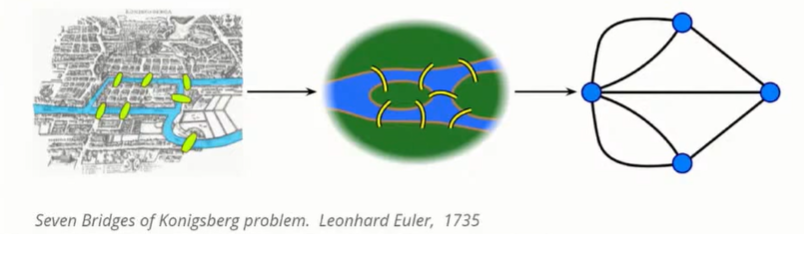
\includegraphics[width=\linewidth,keepaspectratio]{neo4j4}
\end{center}	  

{\tiny (Ref: Introduction to Neo4j - a hands-on crash course - neo4j)}
\end{frame}


%%%%%%%%%%%%%%%%%%%%%%%%%%%%%%%%%%%%%%%%%%%%%%%%%%%%%%%%%%%%%%%%%%%%%%%%%%%%%%%%%%
\begin{frame}\frametitle{Graph Theory}

\begin{itemize}
\item 
\end{itemize}



{\tiny (Ref: A Little Graph Theory for the Busy Developer - Jim Webber GraphConnect London 2013)}
\end{frame}

%%%%%%%%%%%%%%%%%%%%%%%%%%%%%%%%%%%%%%%%%%%%%%%%%%%%%%%%%%%
\begin{frame}[fragile]\frametitle{ Graph-structured Data Are Ubiquitous }

\begin{center}
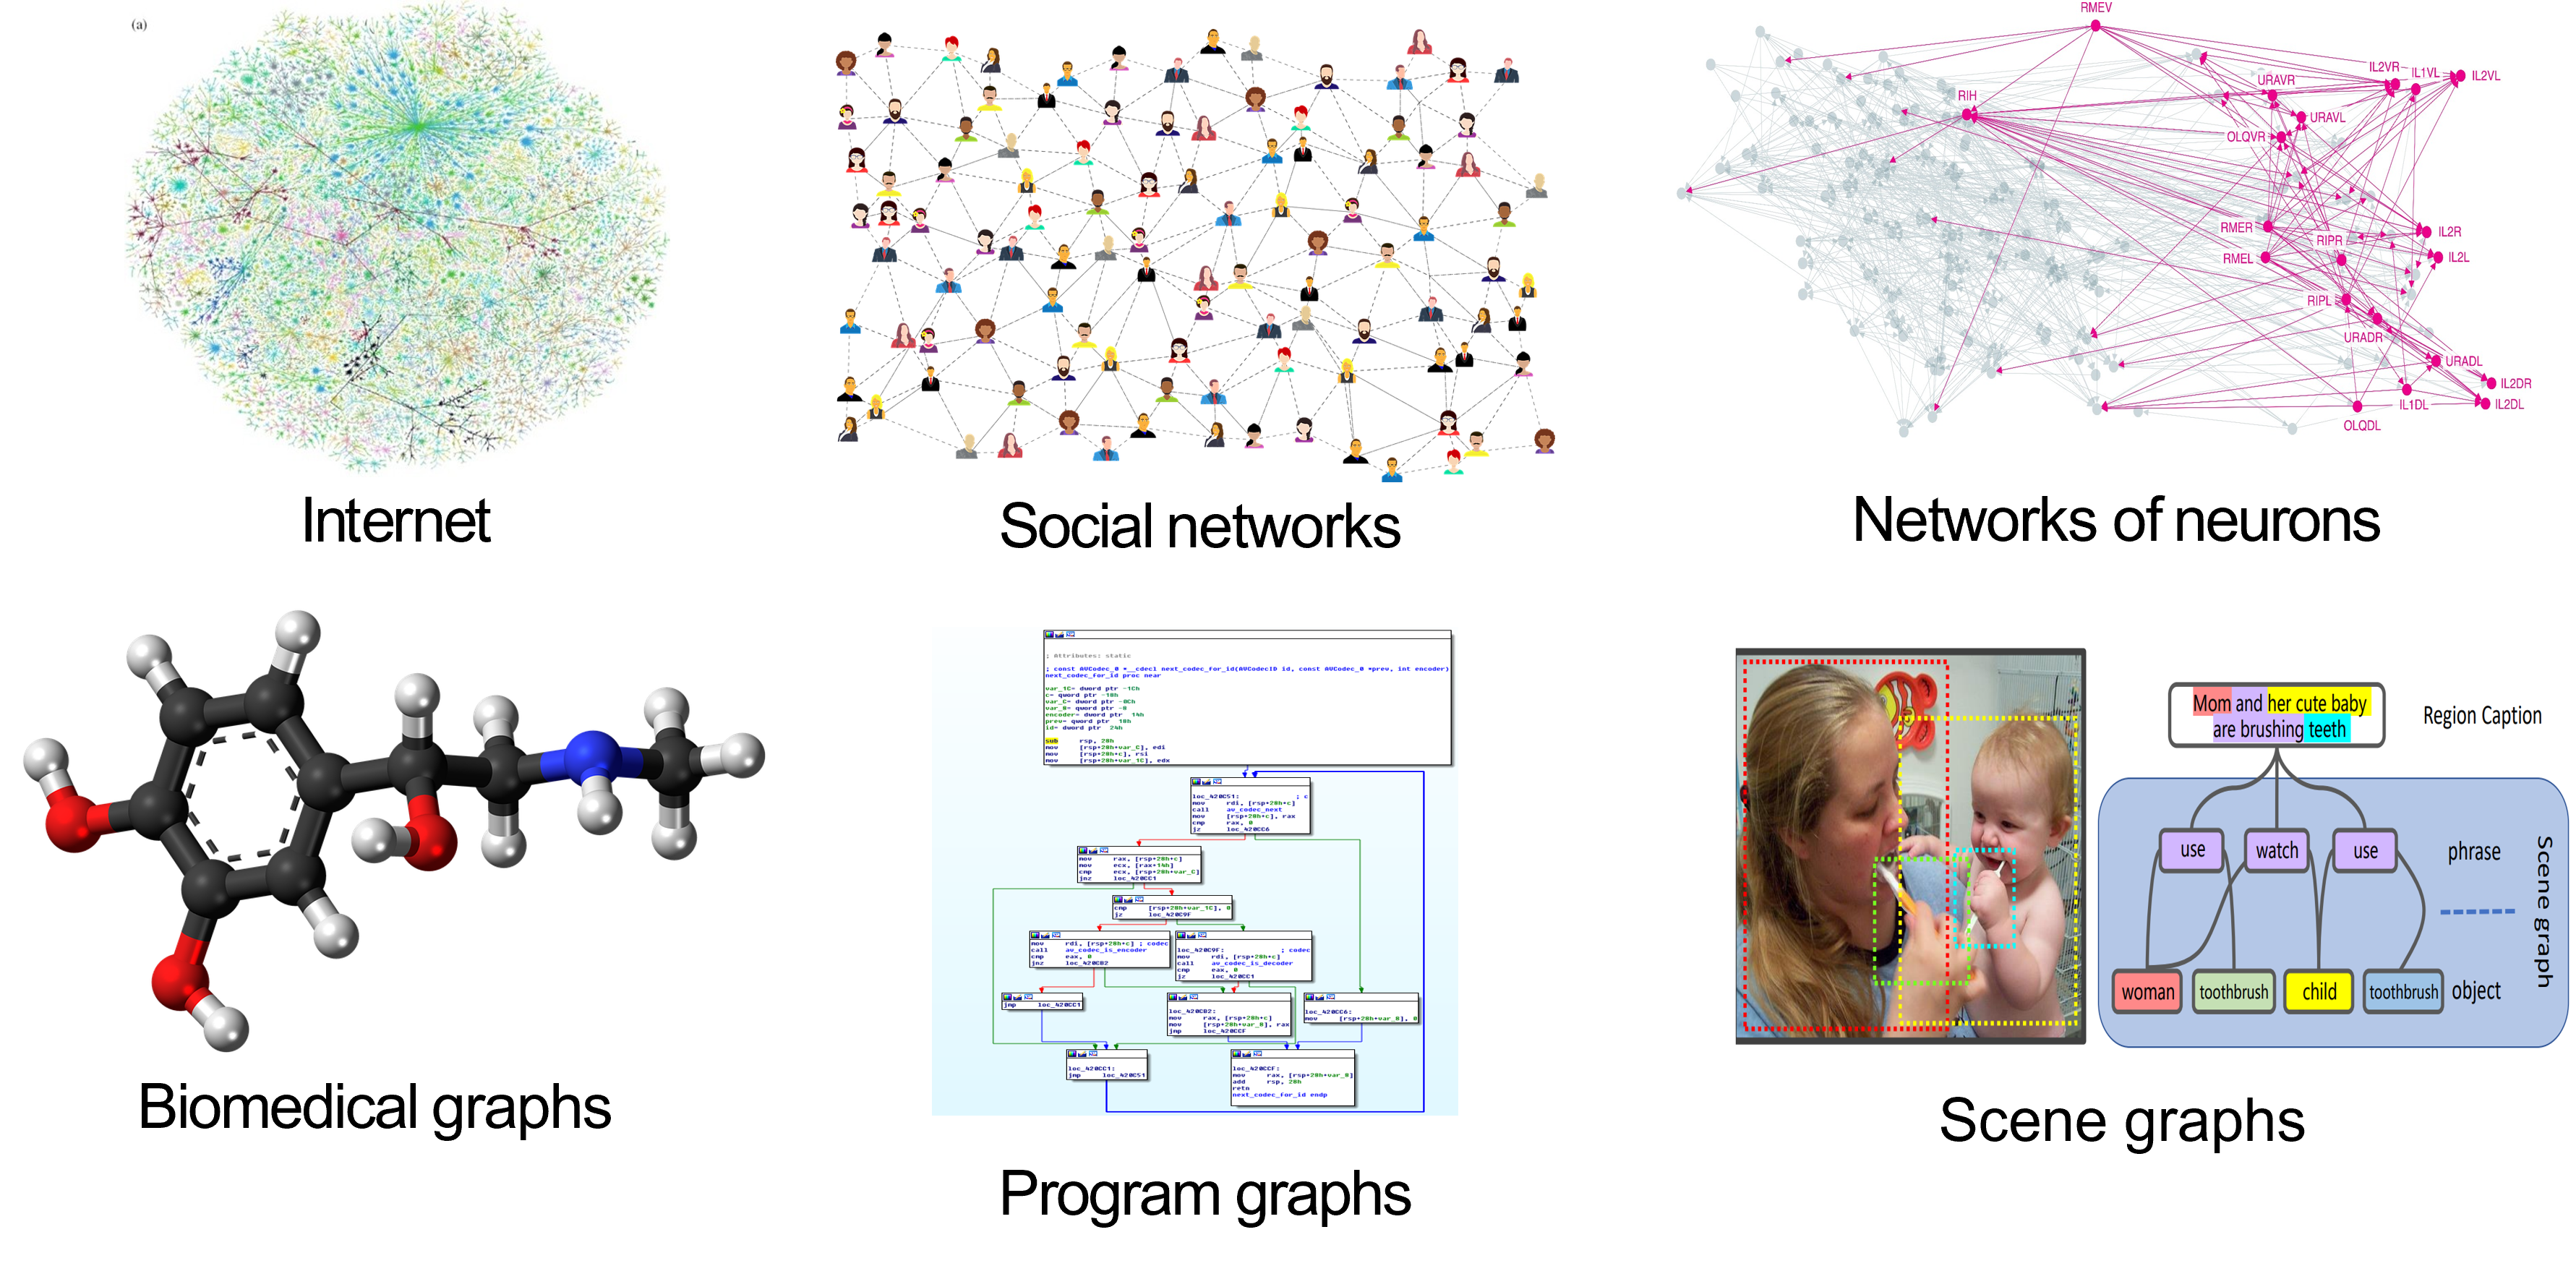
\includegraphics[width=\linewidth,keepaspectratio]{gnn1}
\end{center}	  

\end{frame}

%%%%%%%%%%%%%%%%%%%%%%%%%%%%%%%%%%%%%%%%%%%%%%%%%%%%%%%%%%%
\begin{frame}[fragile]\frametitle{}

\begin{center}
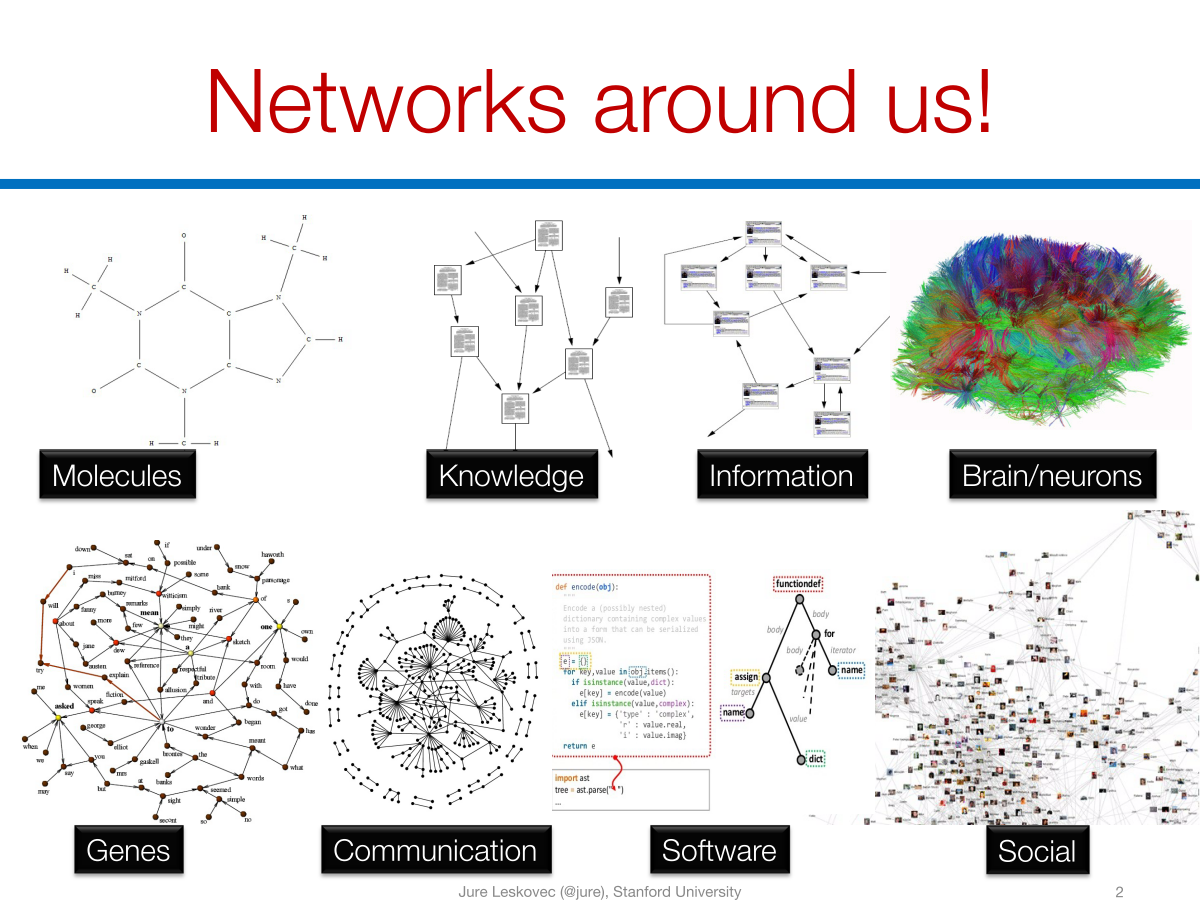
\includegraphics[width=\linewidth,keepaspectratio]{gnn2}
\end{center}	  

\end{frame}

%%%%%%%%%%%%%%%%%%%%%%%%%%%%%%%%%%%%%%%%%%%%%%%%%%%%%%%%%%%
\begin{frame}[fragile]\frametitle{}

\begin{center}
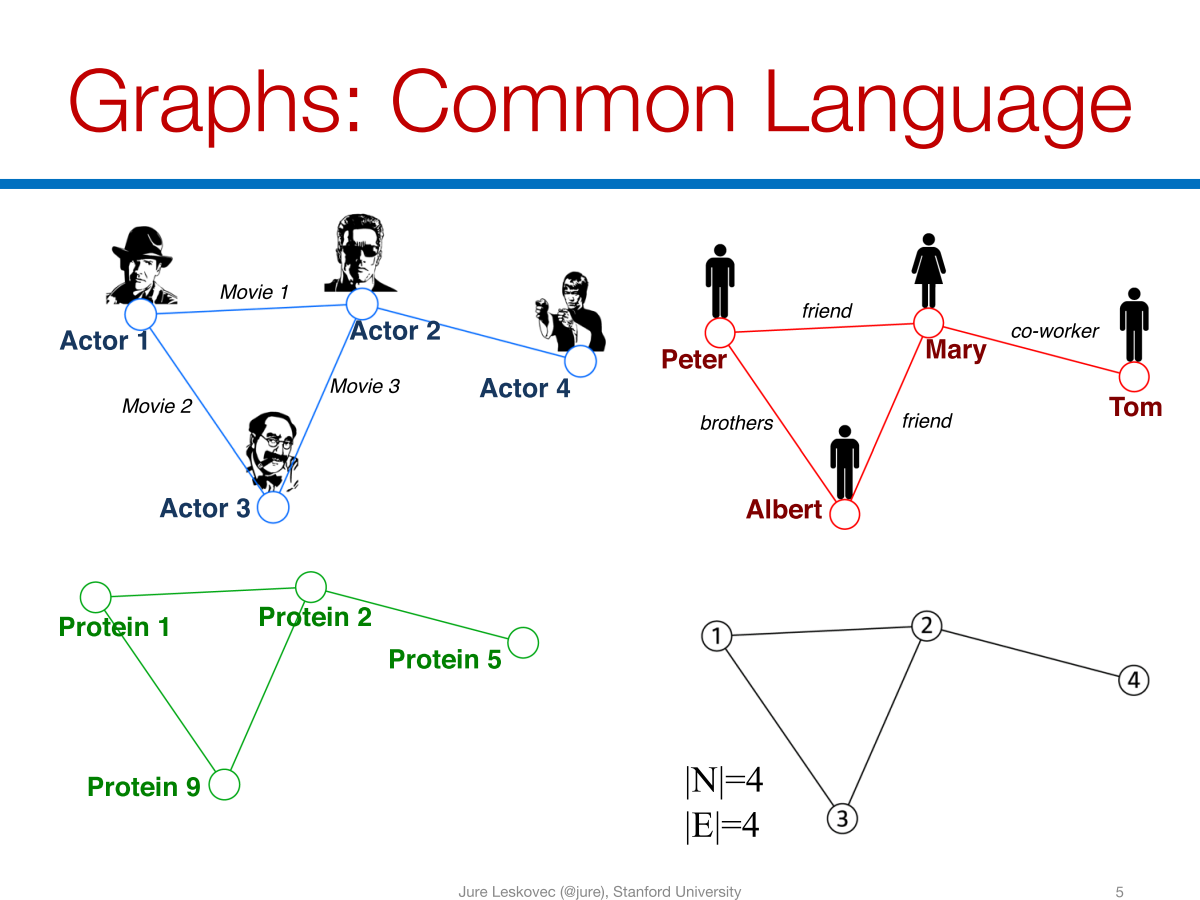
\includegraphics[width=\linewidth,keepaspectratio]{gnn3}
\end{center}	  

\end{frame}

%%%%%%%%%%%%%%%%%%%%%%%%%%%%%%%%%%%%%%%%%%%%%%%%%%%%%%%%%%%
\begin{frame}[fragile]\frametitle{Graphs: A Universal Language }

\begin{center}
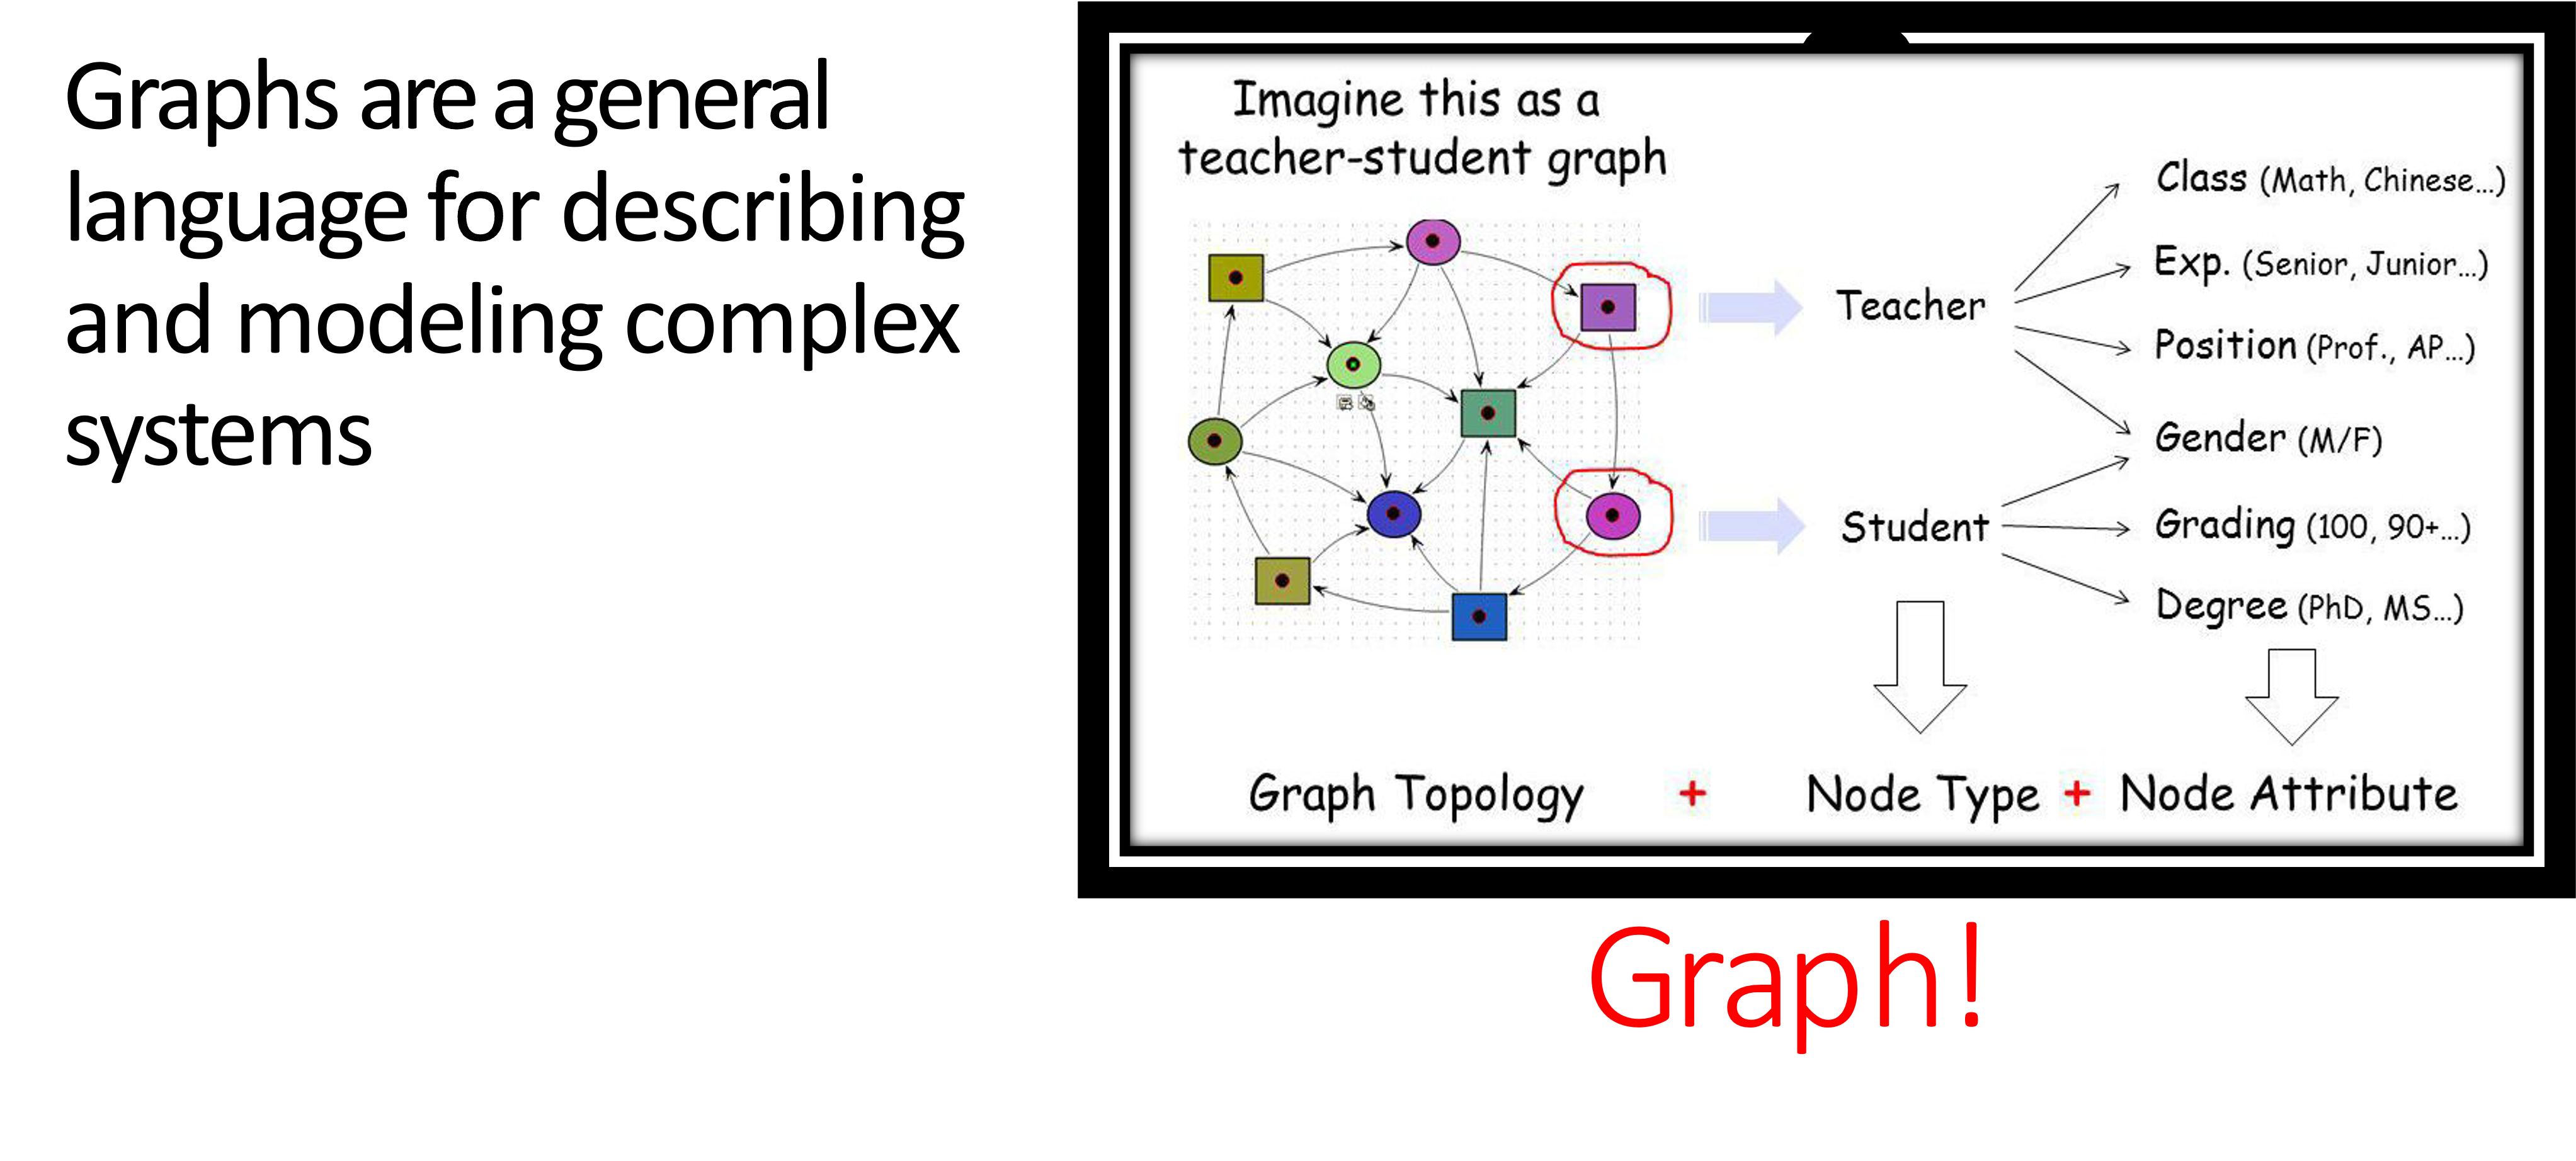
\includegraphics[width=\linewidth,keepaspectratio]{gnn4}
\end{center}	  

\end{frame}


%%%%%%%%%%%%%%%%%%%%%%%%%%%%%%%%%%%%%%%%%%%%%%%%%%%%%%%%%%%
\begin{frame}[fragile]\frametitle{Data as Graphs - Explicit }

\begin{center}
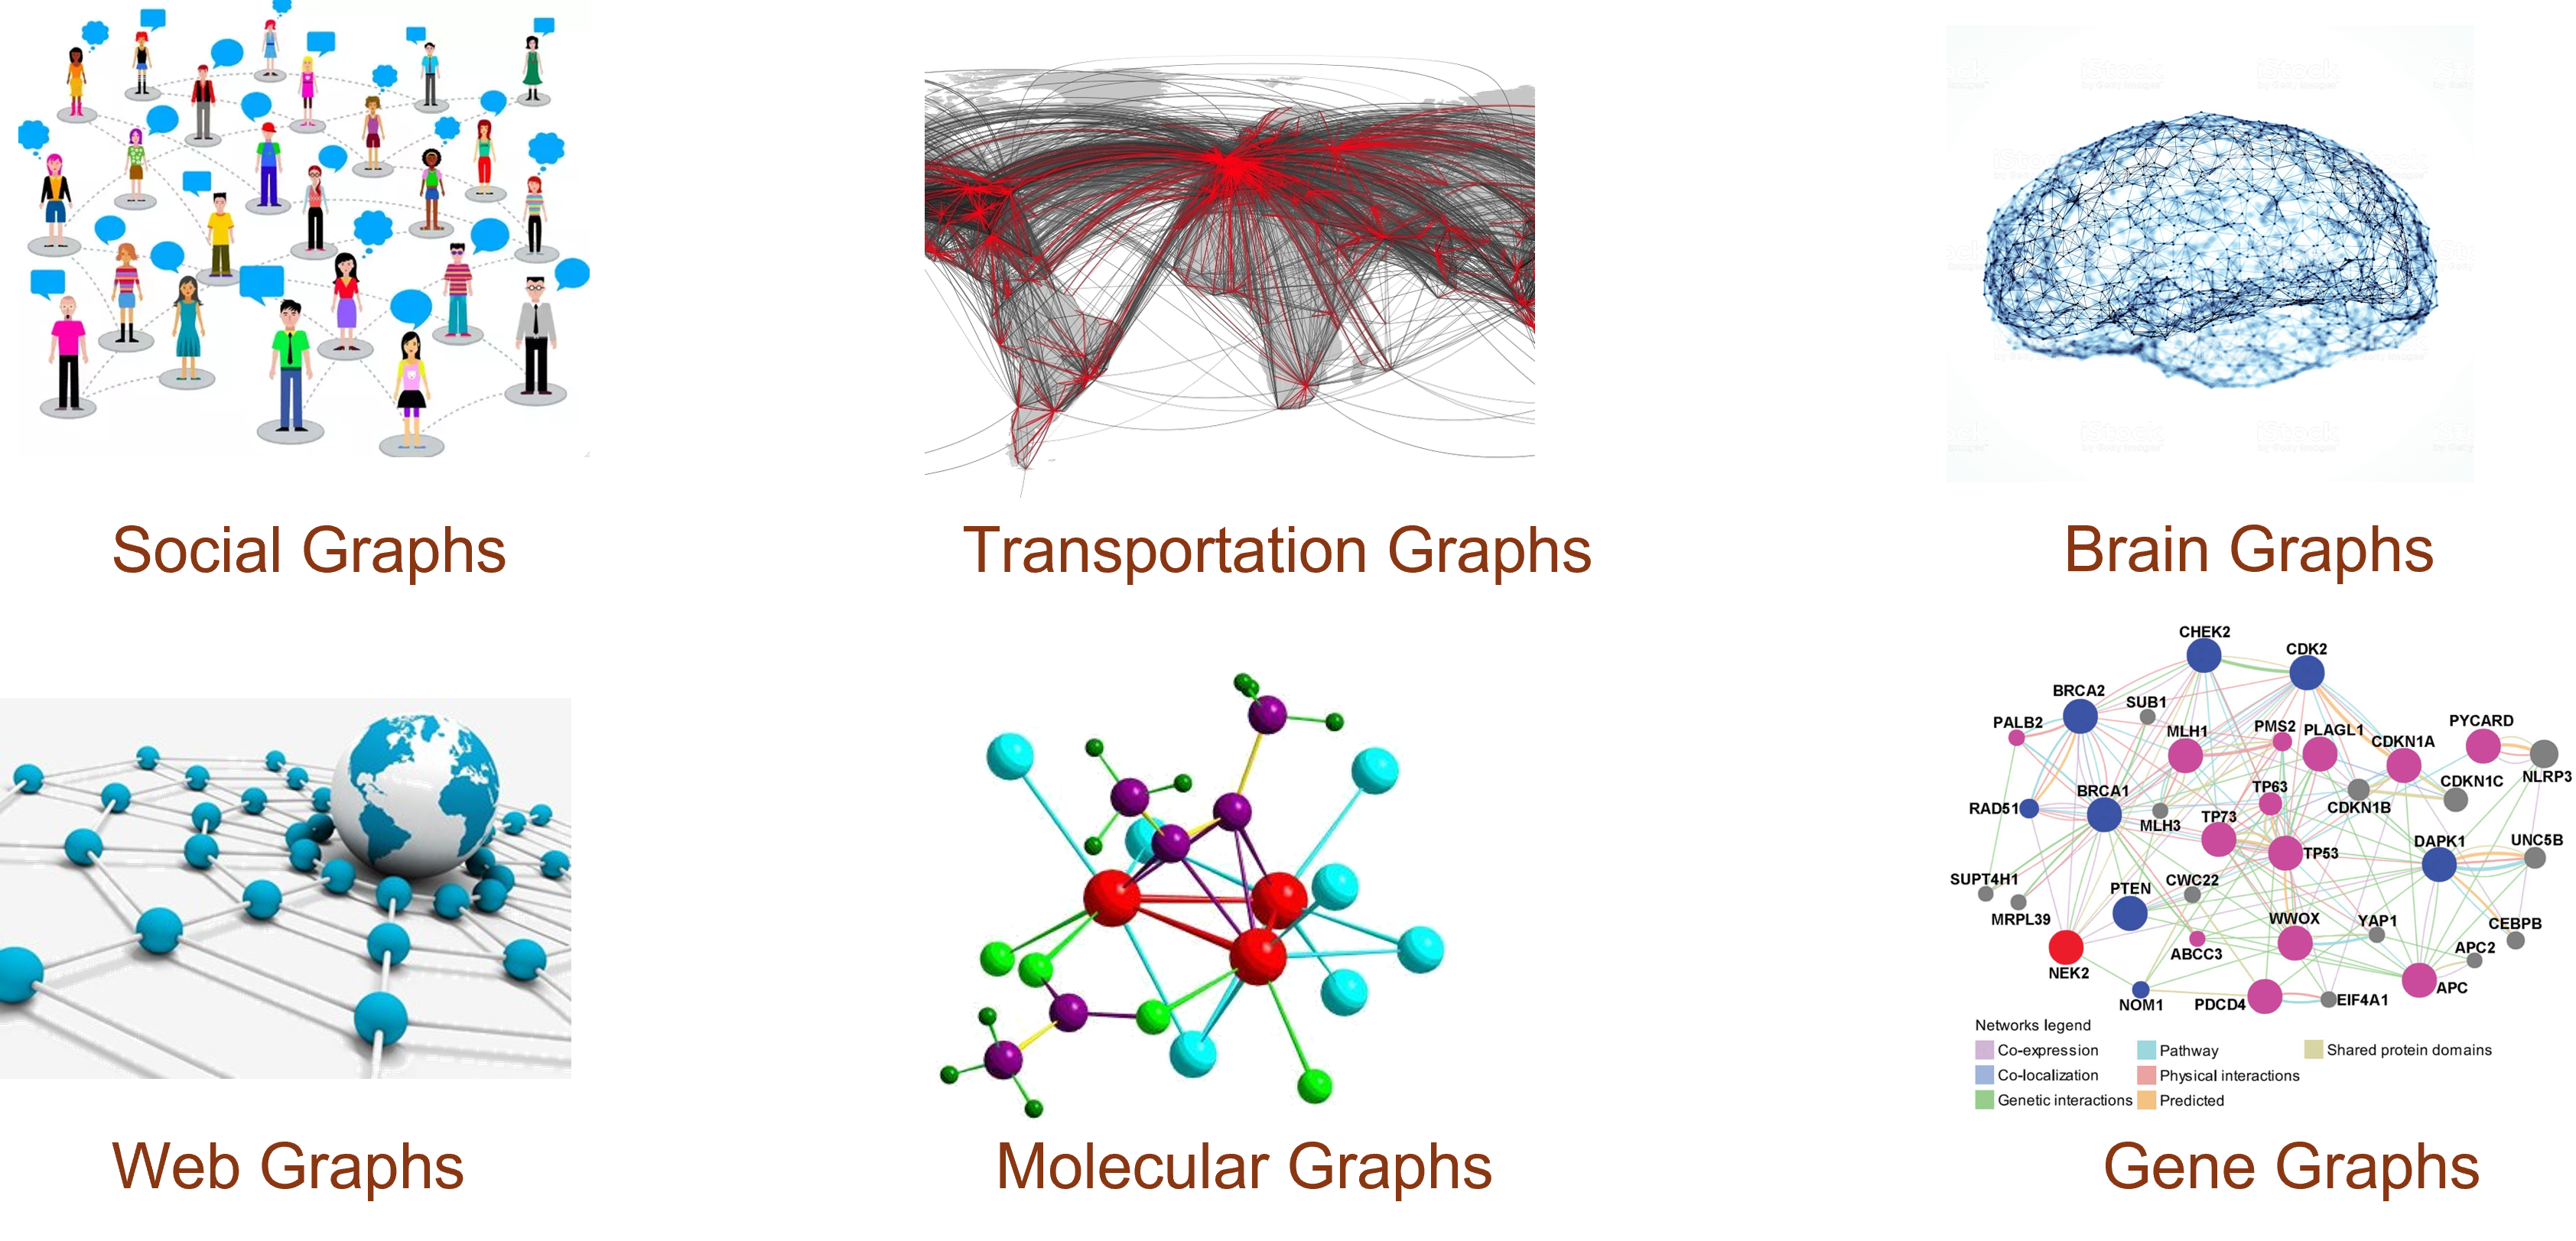
\includegraphics[width=\linewidth,keepaspectratio]{gnn5}
\end{center}	  

\end{frame}

%%%%%%%%%%%%%%%%%%%%%%%%%%%%%%%%%%%%%%%%%%%%%%%%%%%%%%%%%%%
\begin{frame}[fragile]\frametitle{Data as Graphs - Implicit }

\begin{center}
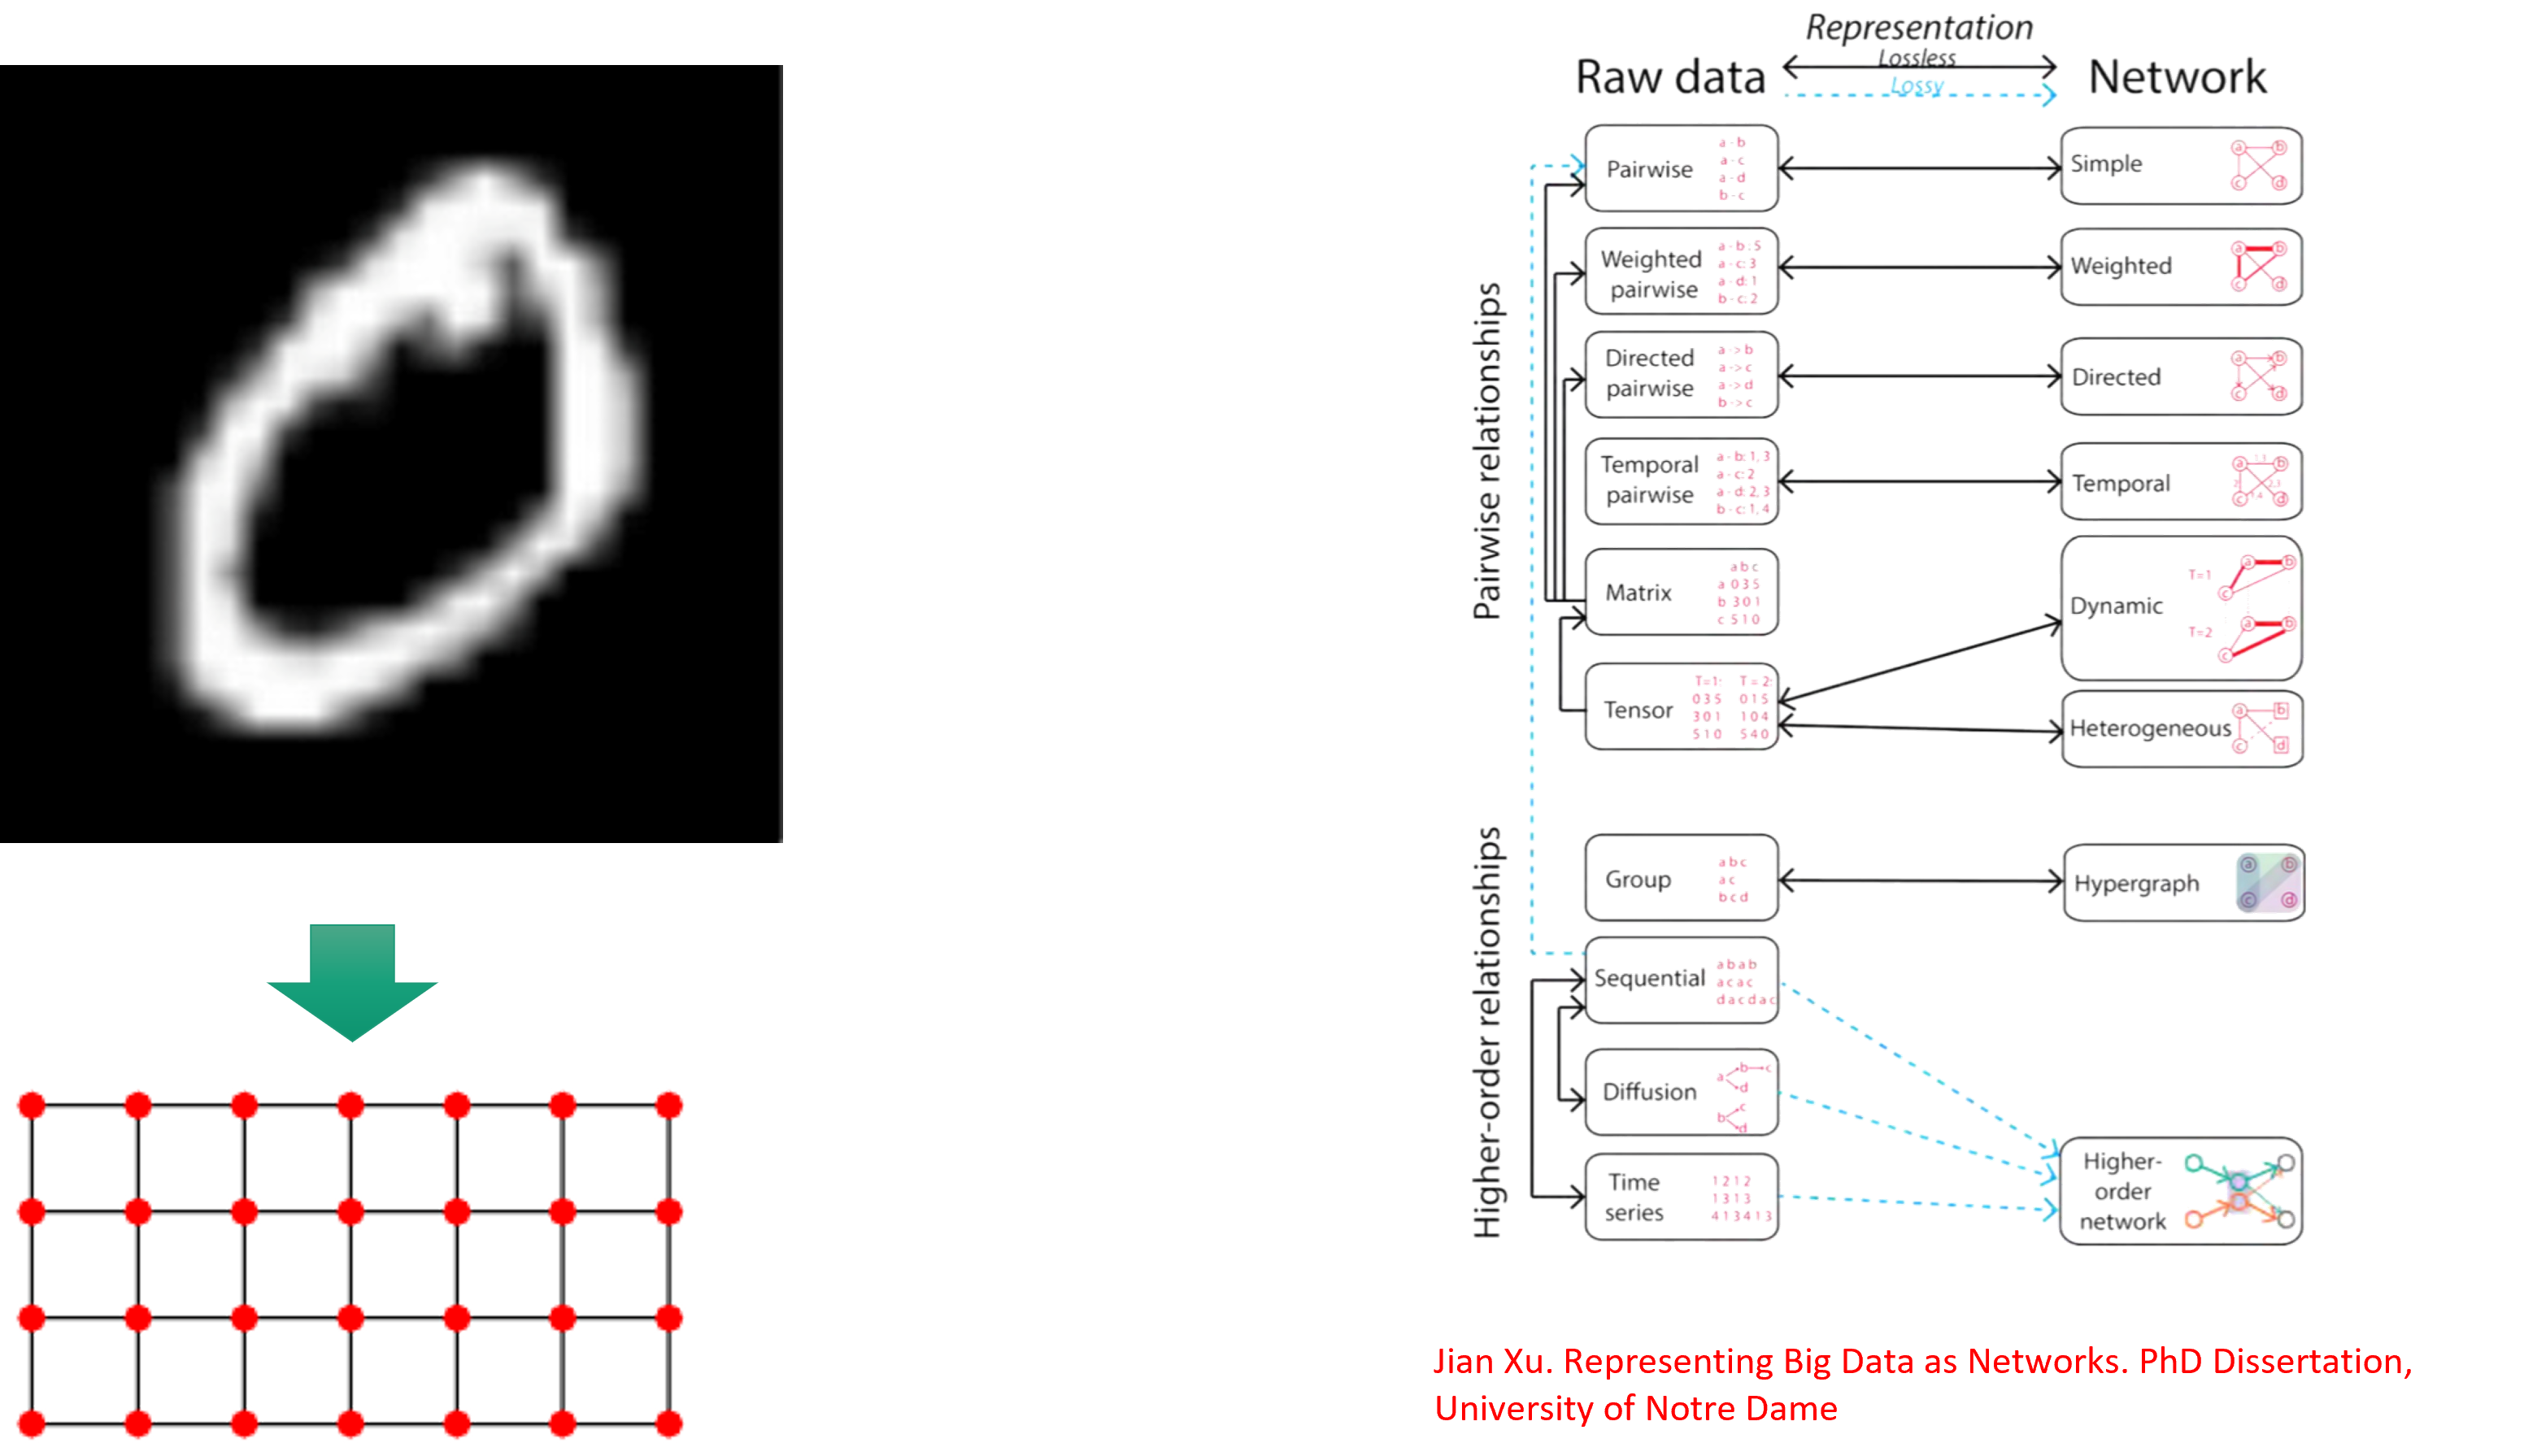
\includegraphics[width=\linewidth,keepaspectratio]{gnn6}
\end{center}	  

\end{frame}



%%%%%%%%%%%%%%%%%%%%%%%%%%%%%%%%%%%%%%%%%%%%%%%%%%%%%%%%%%%
\begin{frame}[fragile]\frametitle{}

\begin{center}
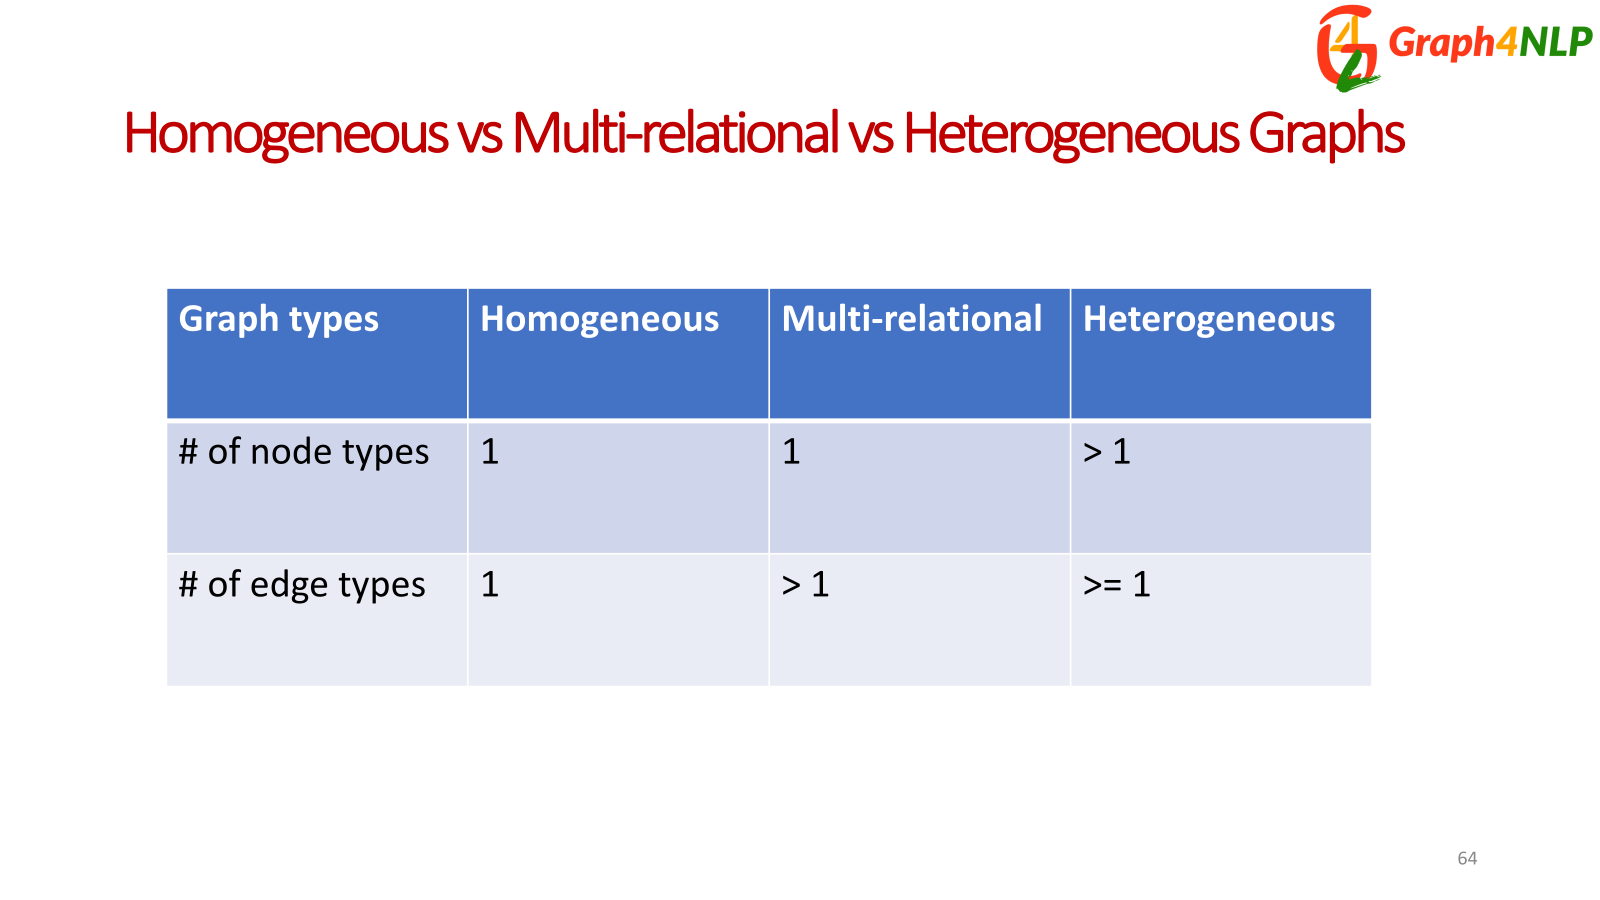
\includegraphics[width=\linewidth,keepaspectratio]{gnn8}
\end{center}	  

\end{frame}


%%%%%%%%%%%%%%%%%%%%%%%%%%%%%%%%%%%%%%%%%%%%%%%%%%%%%%%%%%%%%%%%%%%%%%%%%%%%%%%%%%
\begin{frame}\frametitle{Graph Components}

\begin{itemize}
\item Node (Vertex): A must data element for constructing a graph
\item Relationship (Edge) : Link between two nodes, can have direction and type.
\item Label: Node category/type such as PERSON, ORG, etc. One node can have many types.
\item Properties: Attributes or fields in Nodes or Edges, eg. A node can have Label PERSON and Property such as ``name: Jane''
\end{itemize}



{\tiny (Ref: Introduction to Neo4j - a hands-on crash course - neo4j)}
\end{frame}


%%%%%%%%%%%%%%%%%%%%%%%%%%%%%%%%%%%%%%%%%%%%%%%%%%%%%%%%%%%%%%%%%%%%%%%%%%%%%%%%%%
\begin{frame}\frametitle{Nodes}


\begin{center}
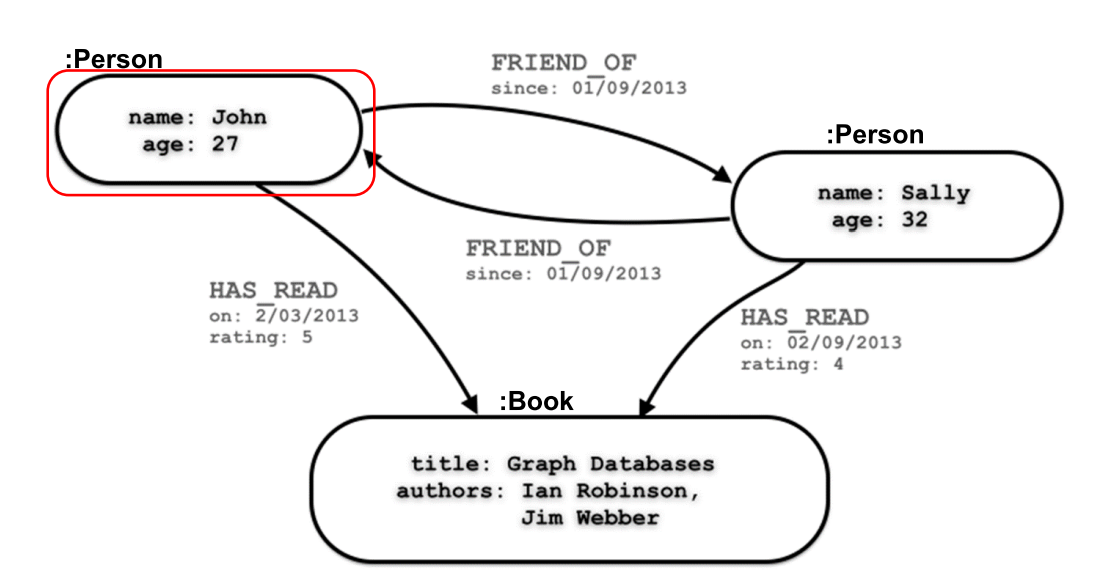
\includegraphics[width=\linewidth,keepaspectratio]{neo4j33}
\end{center}	

{\tiny (Ref: CIS 6930 - Advanced Databases - Neo4j )}
\end{frame}


%%%%%%%%%%%%%%%%%%%%%%%%%%%%%%%%%%%%%%%%%%%%%%%%%%%%%%%%%%%%%%%%%%%%%%%%%%%%%%%%%%
\begin{frame}\frametitle{Relationships}


\begin{center}
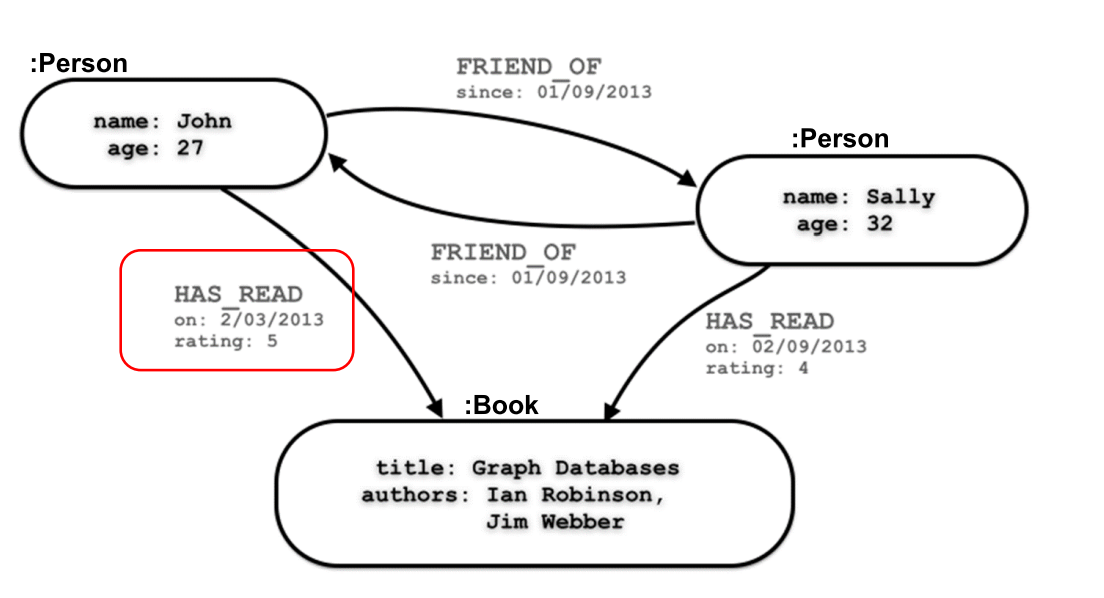
\includegraphics[width=\linewidth,keepaspectratio]{neo4j34}
\end{center}	

{\tiny (Ref: CIS 6930 - Advanced Databases - Neo4j )}
\end{frame}

%%%%%%%%%%%%%%%%%%%%%%%%%%%%%%%%%%%%%%%%%%%%%%%%%%%%%%%%%%%%%%%%%%%%%%%%%%%%%%%%%%
\begin{frame}\frametitle{Properties}


\begin{center}
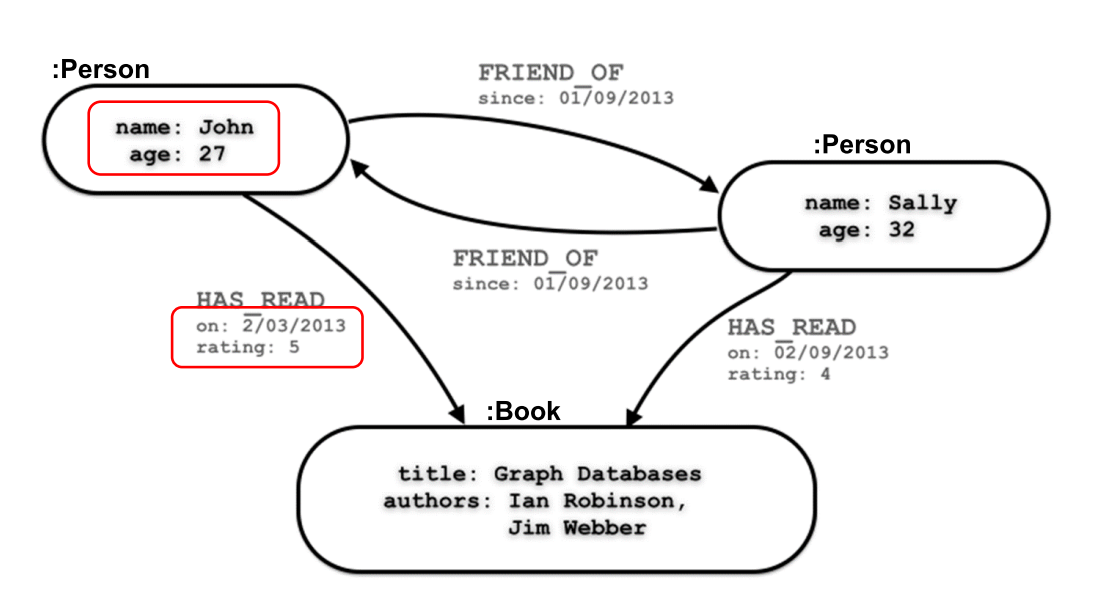
\includegraphics[width=\linewidth,keepaspectratio]{neo4j35}
\end{center}	

{\tiny (Ref: CIS 6930 - Advanced Databases - Neo4j )}
\end{frame}


%%%%%%%%%%%%%%%%%%%%%%%%%%%%%%%%%%%%%%%%%%%%%%%%%%%%%%%%%%%%%%%%%%%%%%%%%%%%%%%%%%
\begin{frame}\frametitle{Labels}


\begin{center}
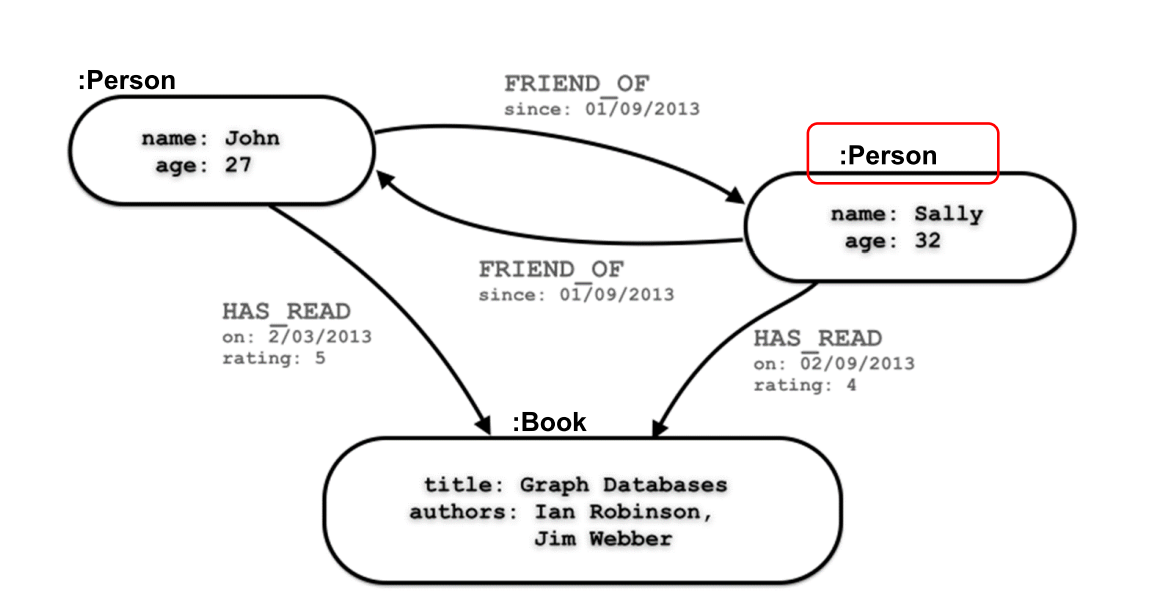
\includegraphics[width=\linewidth,keepaspectratio]{neo4j36}
\end{center}	

{\tiny (Ref: CIS 6930 - Advanced Databases - Neo4j )}
\end{frame}


%%%%%%%%%%%%%%%%%%%%%%%%%%%%%%%%%%%%%%%%%%%%%%%%%%%%%%%%%%%
\begin{frame}[fragile]\frametitle{Graphs and features}

\begin{center}
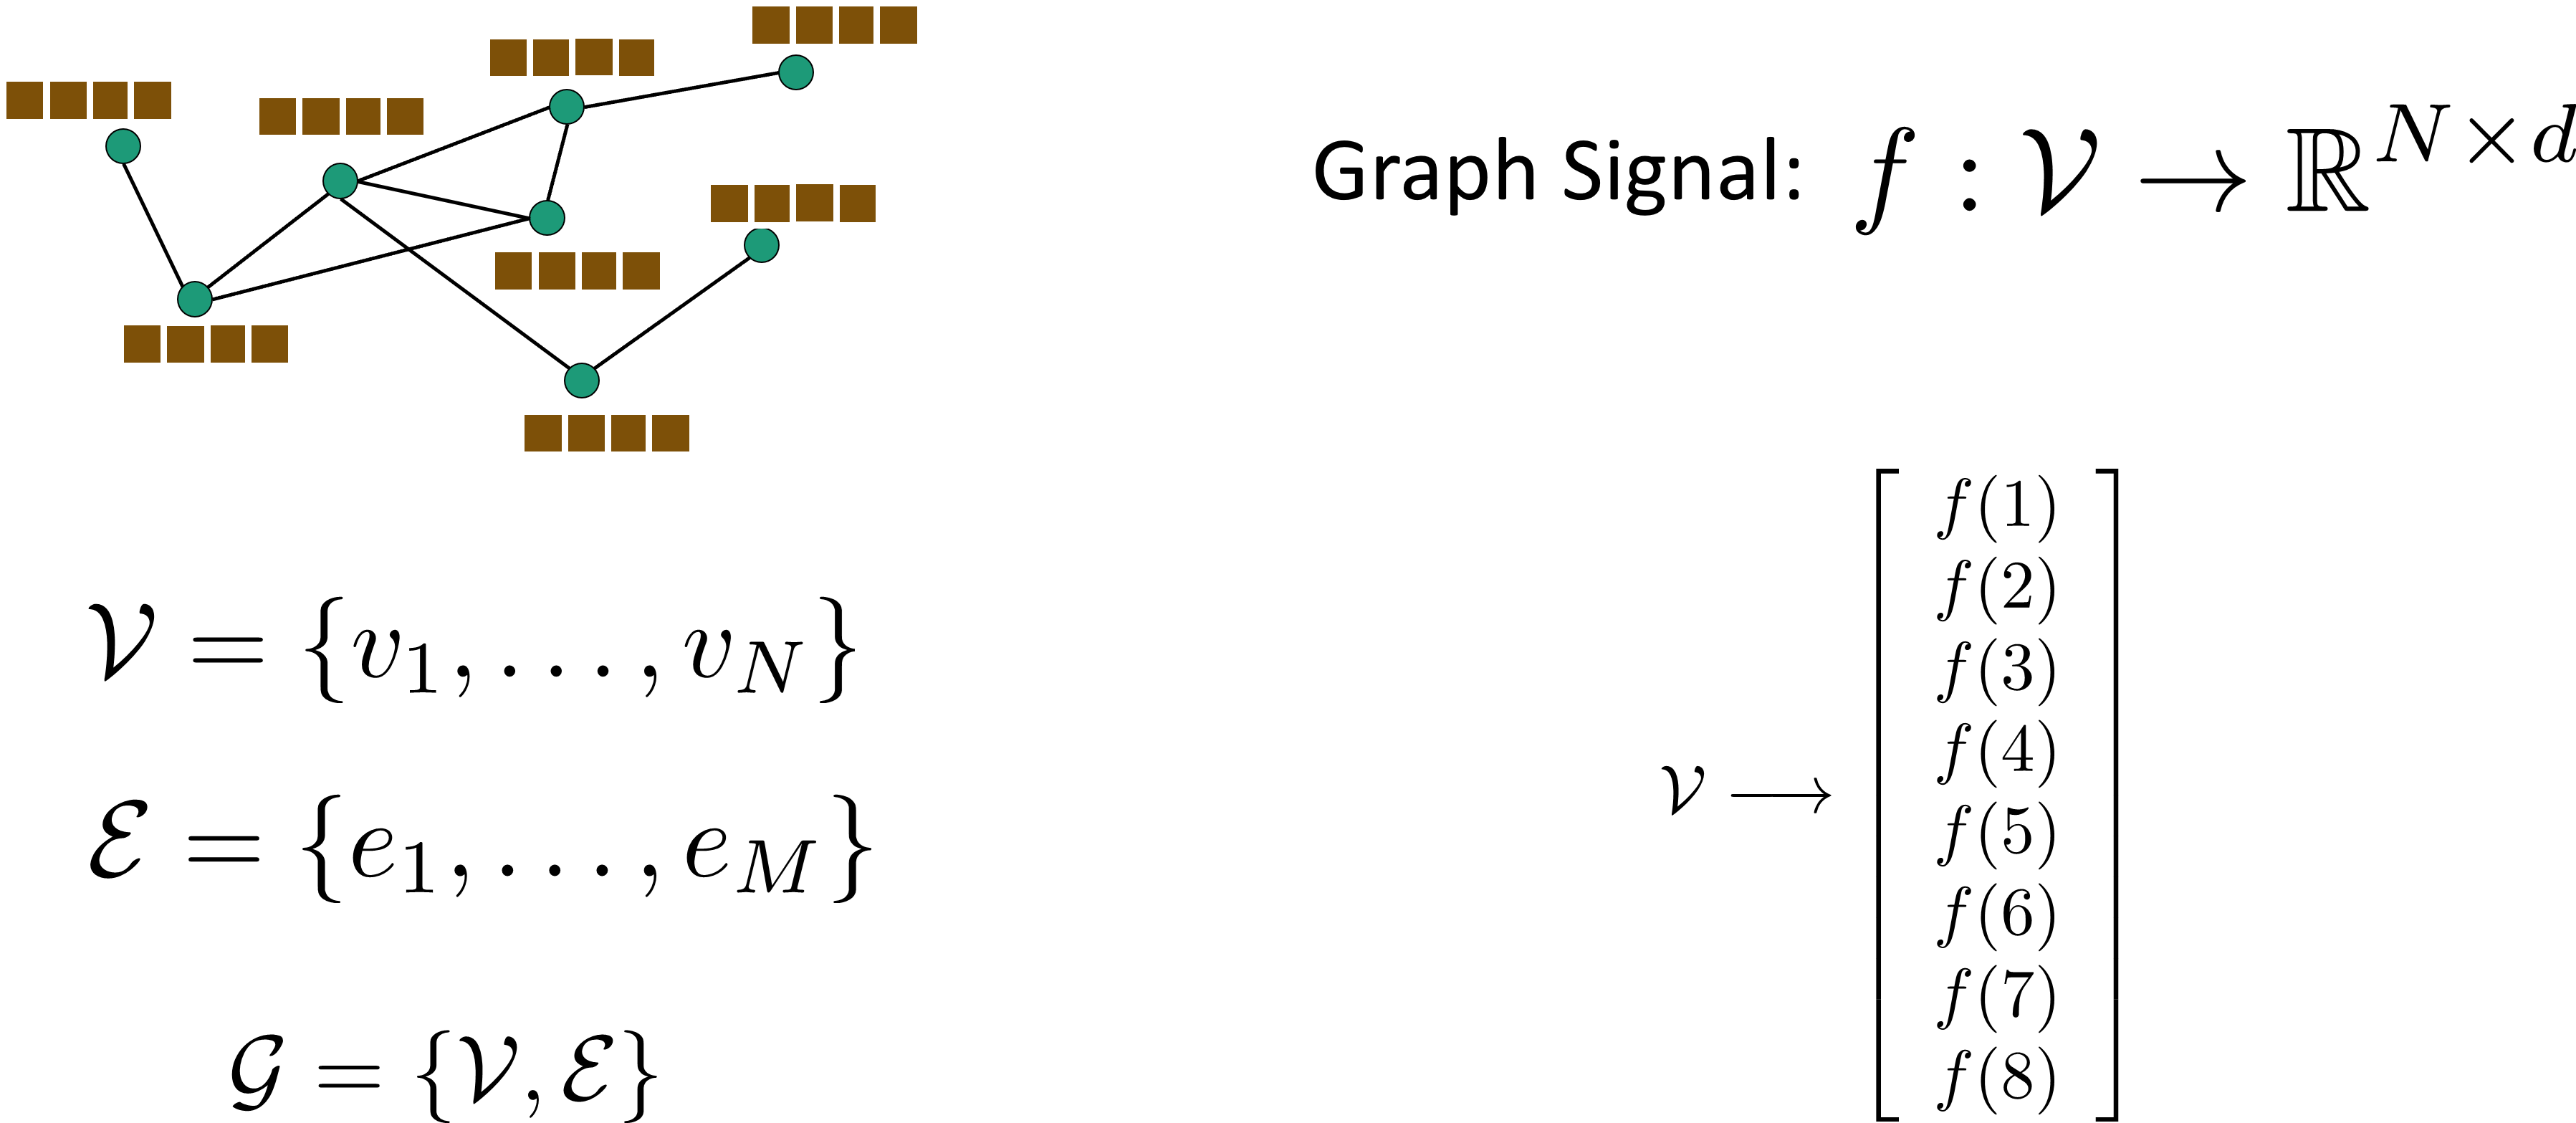
\includegraphics[width=\linewidth,keepaspectratio]{gnn9}
\end{center}	  

\end{frame}

%%%%%%%%%%%%%%%%%%%%%%%%%%%%%%%%%%%%%%%%%%%%%%%%%%%%%%%%%%%
\begin{frame}[fragile]\frametitle{Matrix Representations of Graphs}

\begin{center}
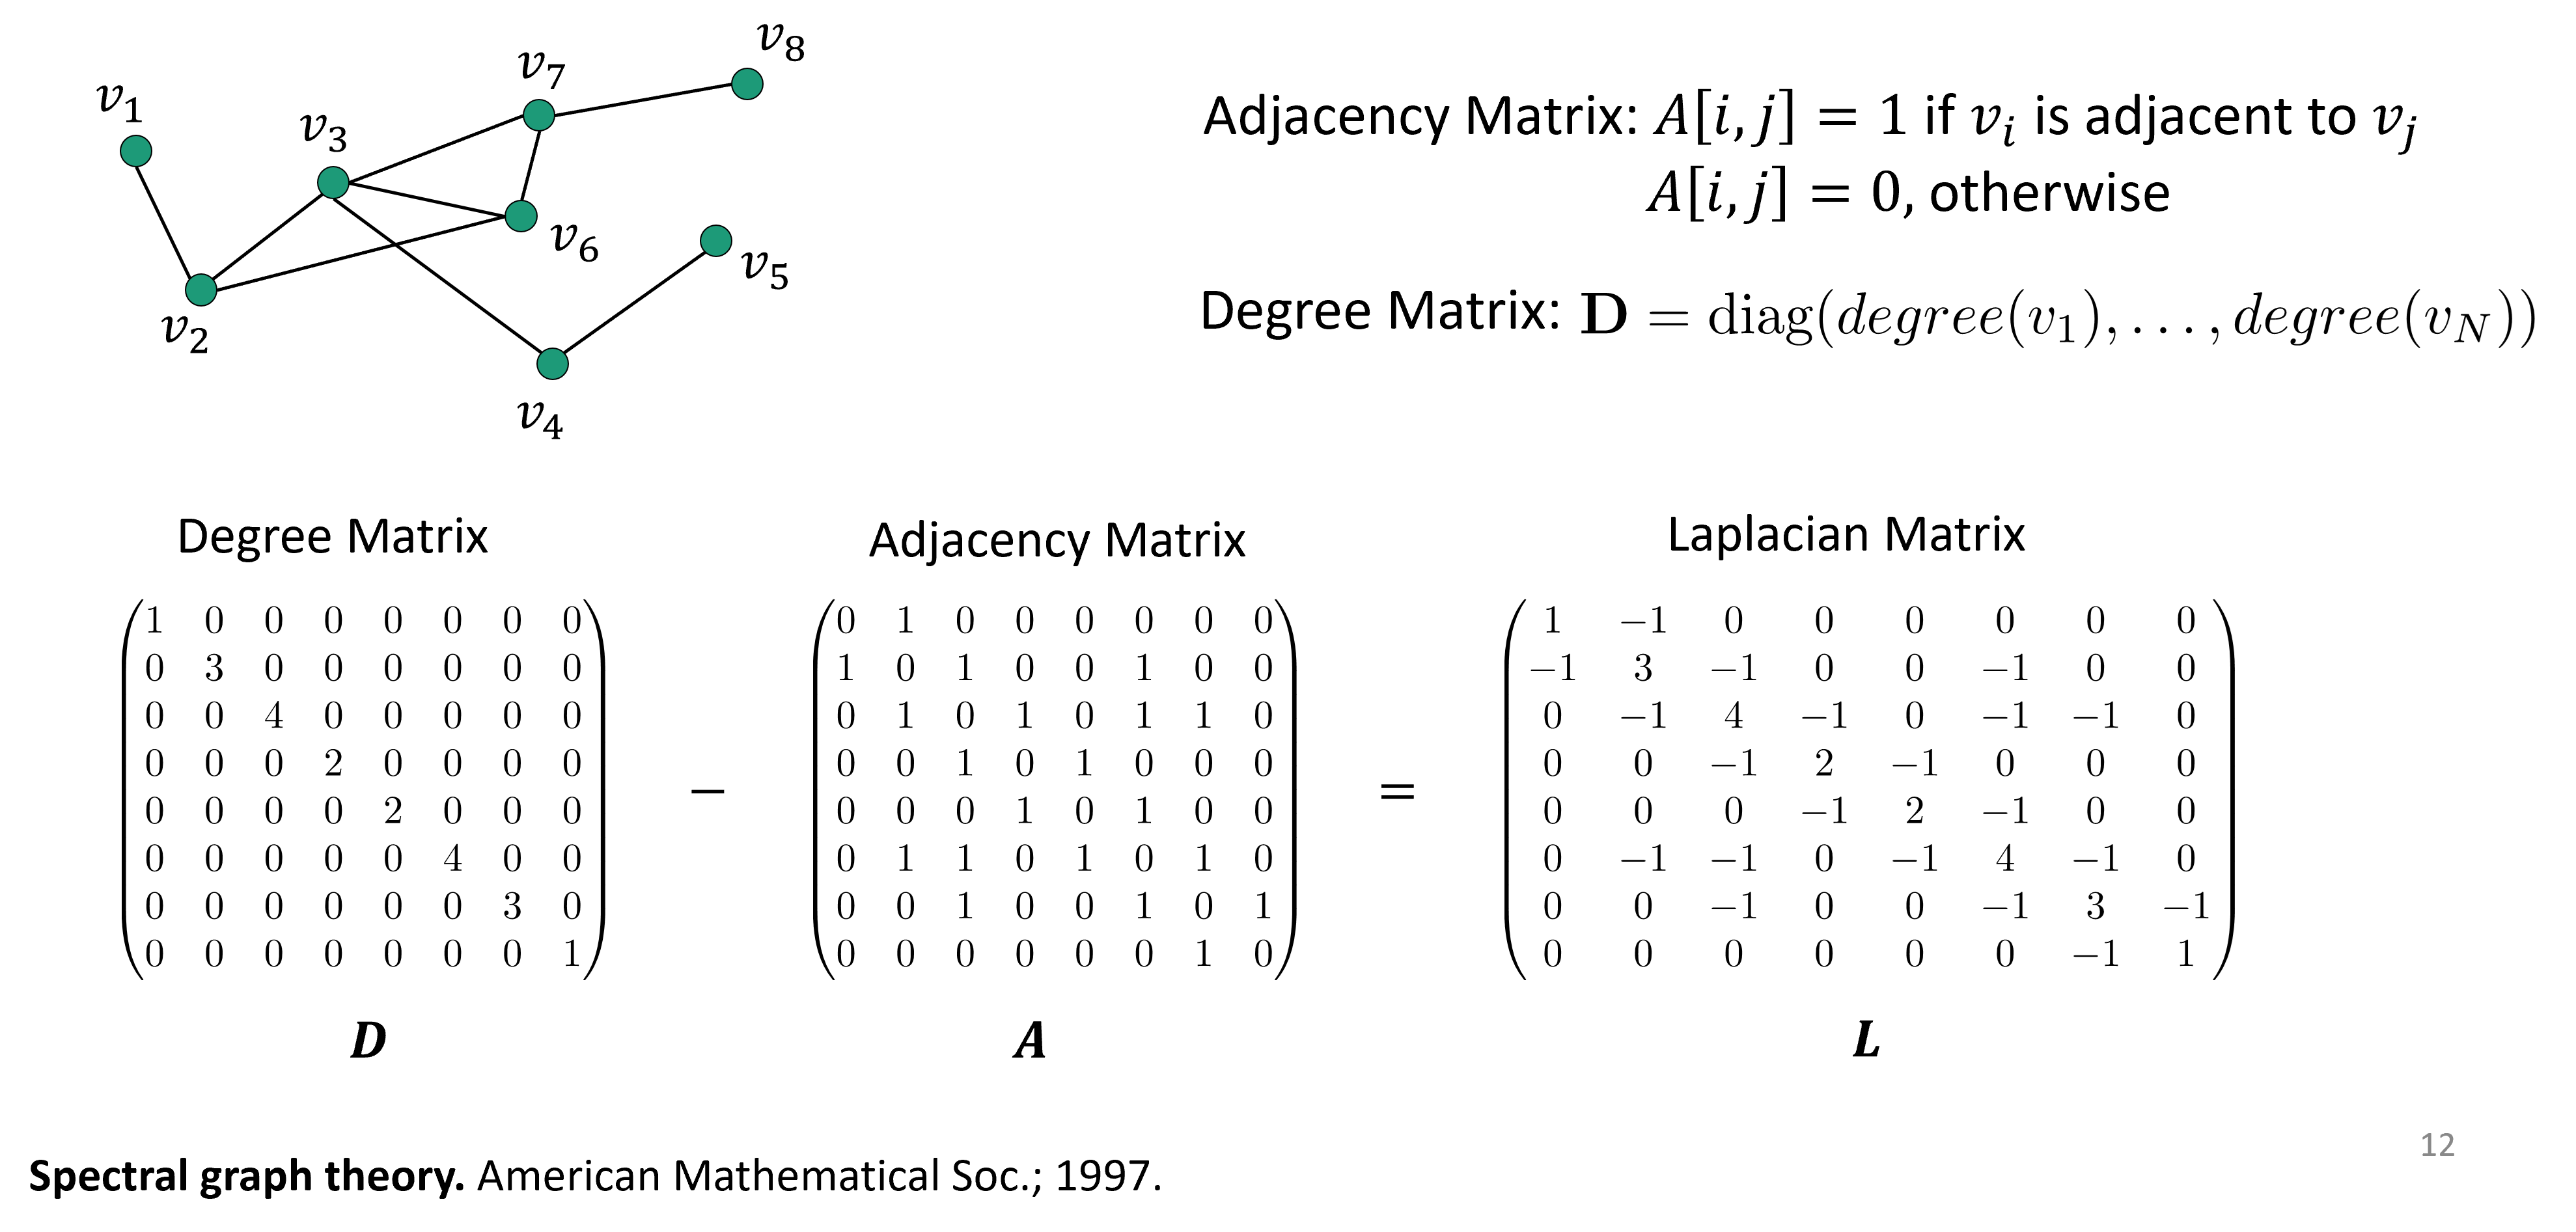
\includegraphics[width=\linewidth,keepaspectratio]{gnn10}
\end{center}	  

\end{frame}

%%%%%%%%%%%%%%%%%%%%%%%%%%%%%%%%%%%%%%%%%%%%%%%%%%%%%%%%%%%
\begin{frame}[fragile]\frametitle{Why Graphs? Why Now?}

\begin{itemize}
\item Universal language for describing complex data: Networks/graphs from science, nature, and technology are more similar than one would expect
\item Shared vocabulary between fields: Computer Science, Social science, Physics, Biology, Economics 
\item Data availability (+ computational challenges): Social/Internet, text, logic, program, bio, health, and medical
\item Impact: Social networking, Social media, Drug design, Event detection, Natural language processing, Computer vision, and Logic reasoning
\end{itemize}

\end{frame}

%%%%%%%%%%%%%%%%%%%%%%%%%%%%%%%%%%%%%%%%%%%%%%%%%%%%%%%%%%%%%%%%%%%%%%%%%%%%%%%%%%
\begin{frame}\frametitle{Identifying good Graph scenarios - 1/4}

Does the problem involve understanding relationships between entities?

Behavioral analysis:

\begin{center}
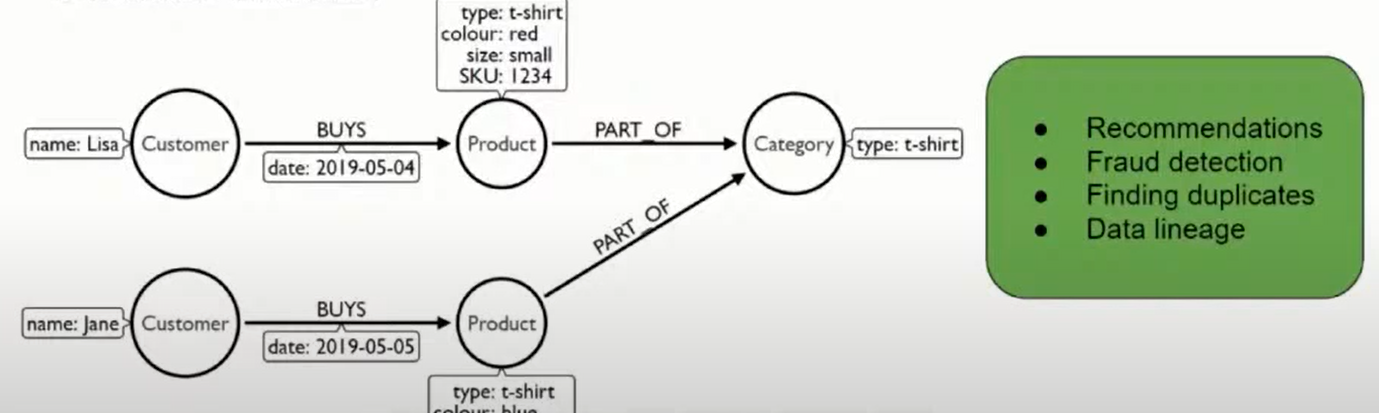
\includegraphics[width=\linewidth,keepaspectratio]{neo4j5}
\end{center}	  

{\tiny (Ref: Introduction to Neo4j - a hands-on crash course - neo4j)}
\end{frame}

%%%%%%%%%%%%%%%%%%%%%%%%%%%%%%%%%%%%%%%%%%%%%%%%%%%%%%%%%%%%%%%%%%%%%%%%%%%%%%%%%%
\begin{frame}\frametitle{Identifying good Graph scenarios - 2/4}

Does the problem involve a lot of self-referencing to the same type of entity?

Org chart of employees:

\begin{center}
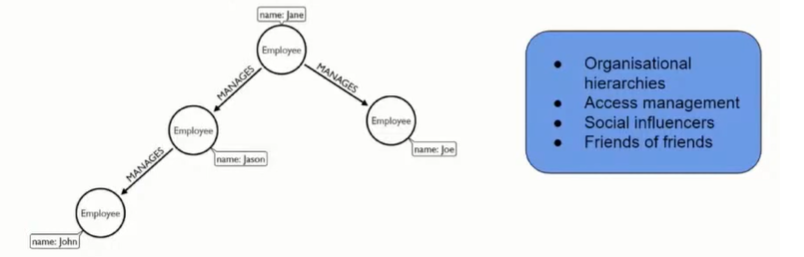
\includegraphics[width=\linewidth,keepaspectratio]{neo4j6}
\end{center}	  

{\tiny (Ref: Introduction to Neo4j - a hands-on crash course - neo4j)}
\end{frame}

%%%%%%%%%%%%%%%%%%%%%%%%%%%%%%%%%%%%%%%%%%%%%%%%%%%%%%%%%%%%%%%%%%%%%%%%%%%%%%%%%%
\begin{frame}\frametitle{Identifying good Graph scenarios - 3/4}

Does the problem explore relationships of varying and unknown depth?

Changes in manufacturing process:

\begin{center}
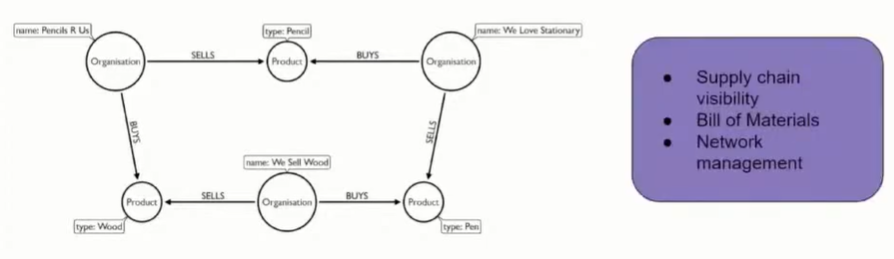
\includegraphics[width=\linewidth,keepaspectratio]{neo4j7}
\end{center}	  

{\tiny (Ref: Introduction to Neo4j - a hands-on crash course - neo4j)}
\end{frame}

%%%%%%%%%%%%%%%%%%%%%%%%%%%%%%%%%%%%%%%%%%%%%%%%%%%%%%%%%%%%%%%%%%%%%%%%%%%%%%%%%%
\begin{frame}\frametitle{Identifying good Graph scenarios - 4/4}

Does the problem involve discovering lots of different routes or paths?

Optimum logistics:

\begin{center}
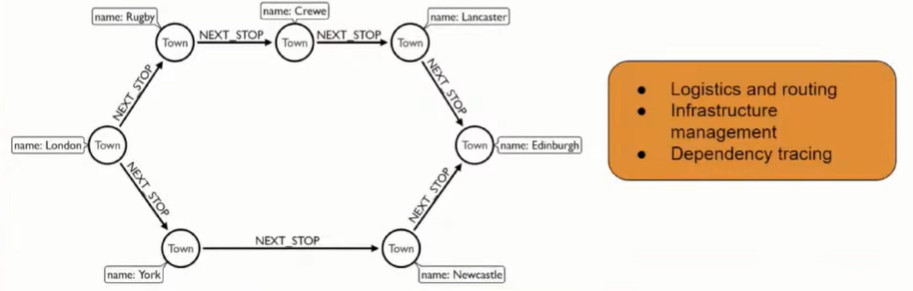
\includegraphics[width=\linewidth,keepaspectratio]{neo4j8}
\end{center}	  

{\tiny (Ref: Introduction to Neo4j - a hands-on crash course - neo4j)}
\end{frame}




% \section[Db]{Databases}
% %%%%%%%%%%%%%%%%%%%%%%%%%%%%%%%%%%%%%%%%%%%%%%%%%%%%%%%%%%%%%%%%%%%%%%%%%%%%%%%%%%
\begin{frame}[fragile]\frametitle{}
\begin{center}
{\Large Database}
\end{center}
\end{frame}


%%%%%%%%%%%%%%%%%%%%%%%%%%%%%%%%%%%%%%%%%%%%%%%%%%%%%%%%%%%%%%%%%%%%%%%%%%%%%%%%%%
\begin{frame}\frametitle{Background}

\begin{itemize}
\item A Database is a place to store application data, to process and query, etc

\item Relational databases (SQL) store data in tables. Strict schema.
\item Document?key-value databases (no-SQL) store data in dictionaries/json. Flexi schema.
\item A Graph Database is where data is stored in graph data structure ie nodes and edges.
\end{itemize}

\begin{center}
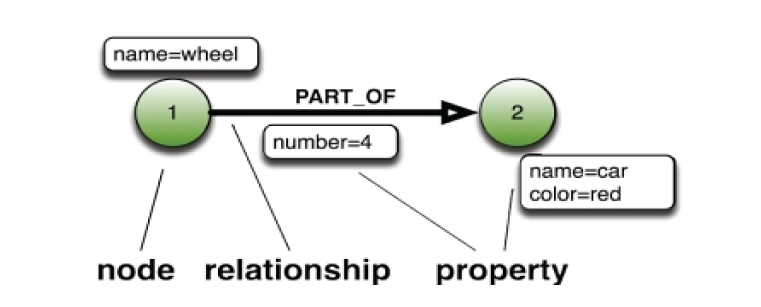
\includegraphics[width=0.5\linewidth,keepaspectratio]{neo4j29}
\end{center}	

{\tiny (Ref: Neo4j (Graph Database) Crash Course - Laith Academy)}
\end{frame}

%%%%%%%%%%%%%%%%%%%%%%%%%%%%%%%%%%%%%%%%%%%%%%%%%%%%%%%%%%%%%%%%%%%%%%%%%%%%%%%%%%
\begin{frame}\frametitle{Example}


\begin{center}
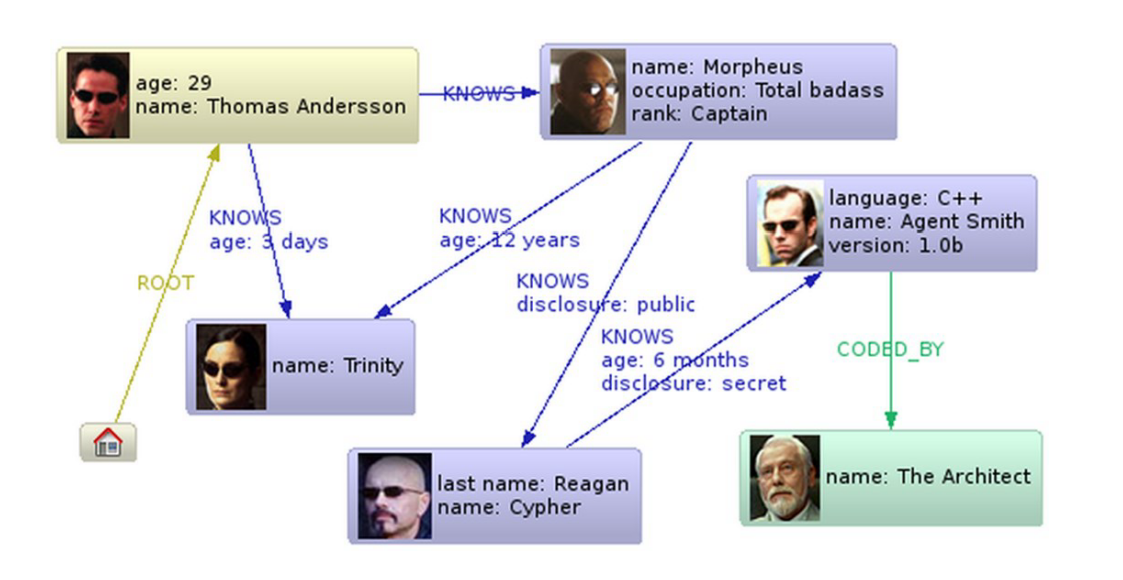
\includegraphics[width=\linewidth,keepaspectratio]{neo4j30}
\end{center}	

{\tiny (Ref: CIS 6930 - Advanced Databases - Neo4j )}
\end{frame}

%%%%%%%%%%%%%%%%%%%%%%%%%%%%%%%%%%%%%%%%%%%%%%%%%%%%%%%%%%%
\begin{frame}[fragile]\frametitle{Relational Database}
SQL

\begin{center}
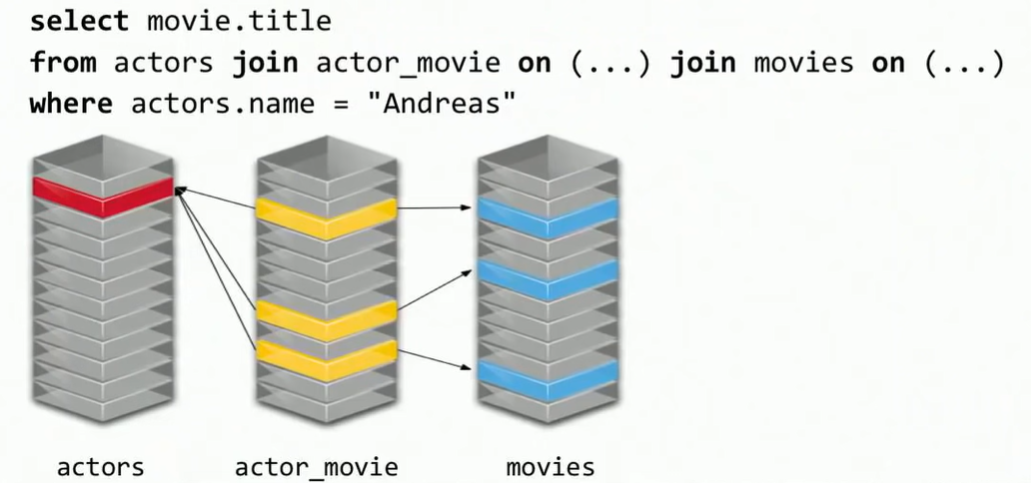
\includegraphics[width=\linewidth,keepaspectratio]{neo4j17}
\end{center}	    

{\tiny (Ref: Introduction to Neo4j and Graph Databases
 - M David Allen)}

\end{frame}

%%%%%%%%%%%%%%%%%%%%%%%%%%%%%%%%%%%%%%%%%%%%%%%%%%%%%%%%%%%
\begin{frame}[fragile]\frametitle{Graph Database}
Cypher

\begin{center}
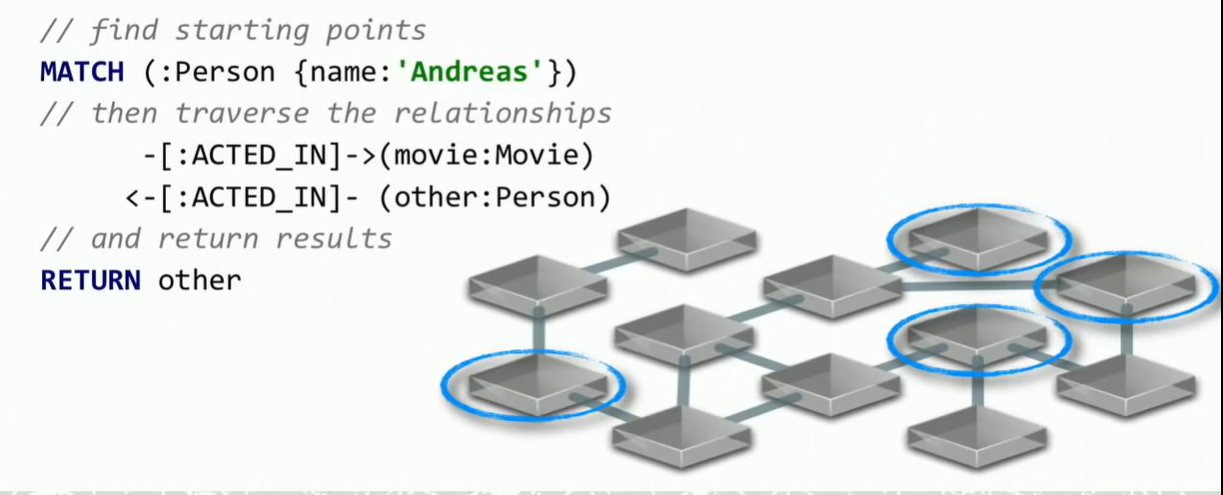
\includegraphics[width=\linewidth,keepaspectratio]{neo4j18}
\end{center}	    

{\tiny (Ref: Introduction to Neo4j and Graph Databases
 - M David Allen)}

\end{frame}

%%%%%%%%%%%%%%%%%%%%%%%%%%%%%%%%%%%%%%%%%%%%%%%%%%%%%%%%%%%%%%%%%%%%%%%%%%%%%%%%%%
\begin{frame}\frametitle{RDBMS}

\begin{itemize}
\item Cannot model or store data and relationships well, ie, without complexity
\item Performance degrades with umber and levels of relationships and database size
\item Query complexity grows with the need for JOINs
\item Adding new types of data and relationships requires schema redesign
\item More difficult if that needs to be done real time.
\end{itemize}

{\tiny (Ref: Neo4j (Graph Database) Crash Course - Laith Academy)}
\end{frame}

%%%%%%%%%%%%%%%%%%%%%%%%%%%%%%%%%%%%%%%%%%%%%%%%%%%%%%%%%%%
\begin{frame}[fragile]\frametitle{Comparison}
Find all reports and how many people they manage upto 3 levels down.

\begin{center}
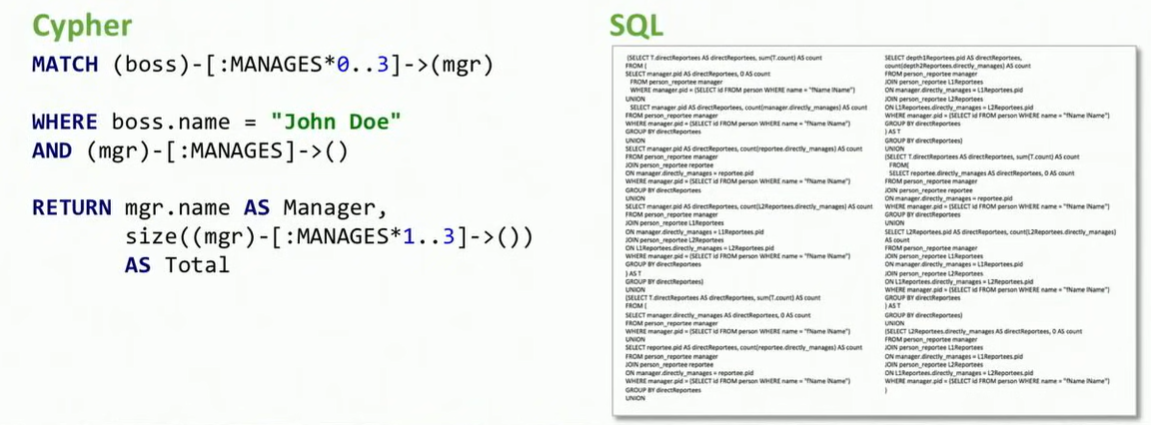
\includegraphics[width=\linewidth,keepaspectratio]{neo4j19}
\end{center}	    

{\tiny (Ref: Introduction to Neo4j and Graph Databases
 - M David Allen)}

\end{frame}

%%%%%%%%%%%%%%%%%%%%%%%%%%%%%%%%%%%%%%%%%%%%%%%%%%%%%%%%%%%
\begin{frame}[fragile]\frametitle{Same Data, Different Layout}
No more Tables, no more Doreign Keys, no more Joins
\begin{center}
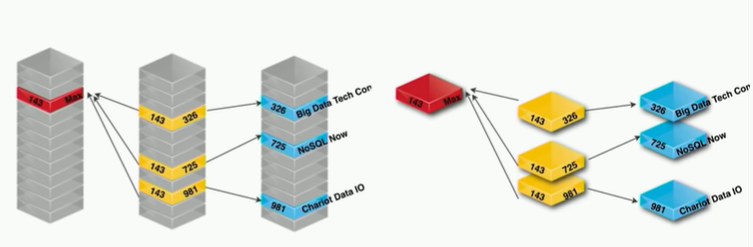
\includegraphics[width=\linewidth,keepaspectratio]{neo4j22}
\end{center}	    

{\tiny (Ref: Secret Sauce of Neo4j: Modeling and Querying Graphs
 - Max De Marzi )}

\end{frame}

%%%%%%%%%%%%%%%%%%%%%%%%%%%%%%%%%%%%%%%%%%%%%%%%%%%%%%%%%%%
\begin{frame}[fragile]\frametitle{Relational Databases cannot do Relationships}

\begin{center}
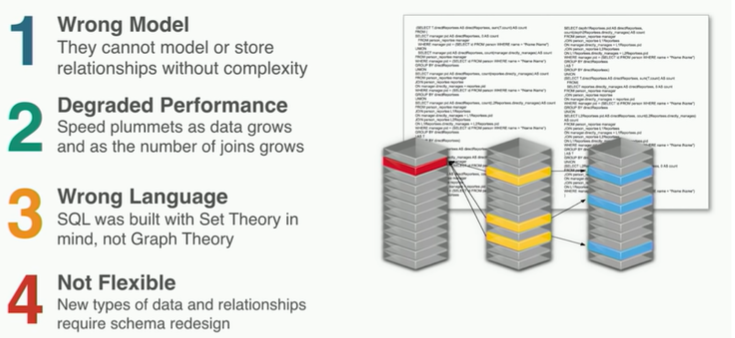
\includegraphics[width=\linewidth,keepaspectratio]{neo4j23}
\end{center}	    

{\tiny (Ref: Secret Sauce of Neo4j: Modeling and Querying Graphs
 - Max De Marzi )}

\end{frame}

%%%%%%%%%%%%%%%%%%%%%%%%%%%%%%%%%%%%%%%%%%%%%%%%%%%%%%%%%%%
\begin{frame}[fragile]\frametitle{No-SQL Databases cannot do Relationships}
Key-value pairs, no Joins, no connections

\begin{center}
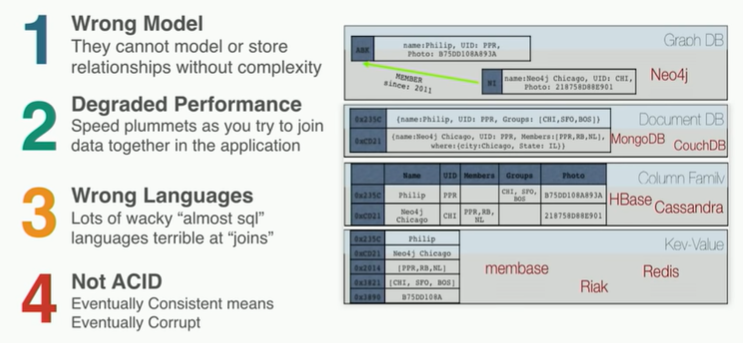
\includegraphics[width=\linewidth,keepaspectratio]{neo4j24}
\end{center}	    

{\tiny (Ref: Secret Sauce of Neo4j: Modeling and Querying Graphs
 - Max De Marzi )}

\end{frame}

%%%%%%%%%%%%%%%%%%%%%%%%%%%%%%%%%%%%%%%%%%%%%%%%%%%%%%%%%%%
\begin{frame}[fragile]\frametitle{Performance}
Remains steady as Database grows. Btw, suitable for graph like data only, and not like lists-queues like dataset where RDBM will work far better.

\begin{center}
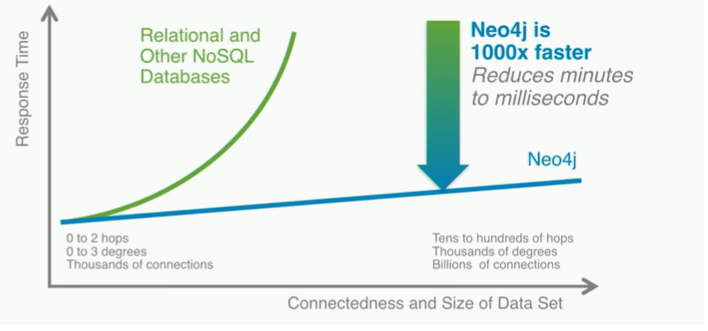
\includegraphics[width=\linewidth,keepaspectratio]{neo4j25}
\end{center}	    

{\tiny (Ref: Secret Sauce of Neo4j: Modeling and Querying Graphs
 - Max De Marzi )}

\end{frame}

%%%%%%%%%%%%%%%%%%%%%%%%%%%%%%%%%%%%%%%%%%%%%%%%%%%%%%%%%%%
\begin{frame}[fragile]\frametitle{Smells like a Graph?}

\begin{center}
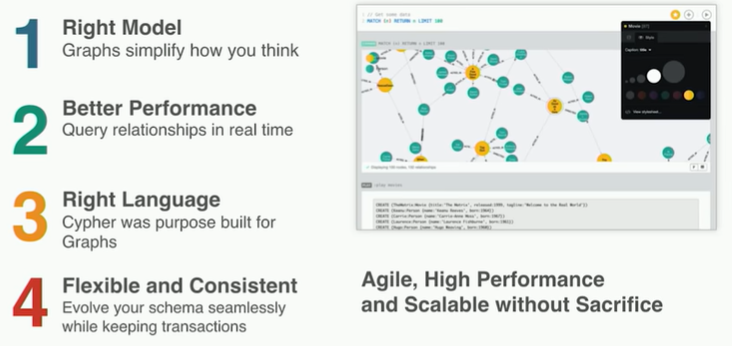
\includegraphics[width=\linewidth,keepaspectratio]{neo4j26}
\end{center}	    

{\tiny (Ref: Secret Sauce of Neo4j: Modeling and Querying Graphs
 - Max De Marzi )}

\end{frame}

%%%%%%%%%%%%%%%%%%%%%%%%%%%%%%%%%%%%%%%%%%%%%%%%%%%%%%%%%%%%%%%%%%%%%%%%%%%%%%%%%%
\begin{frame}\frametitle{Successful companies using graphs}


\begin{center}
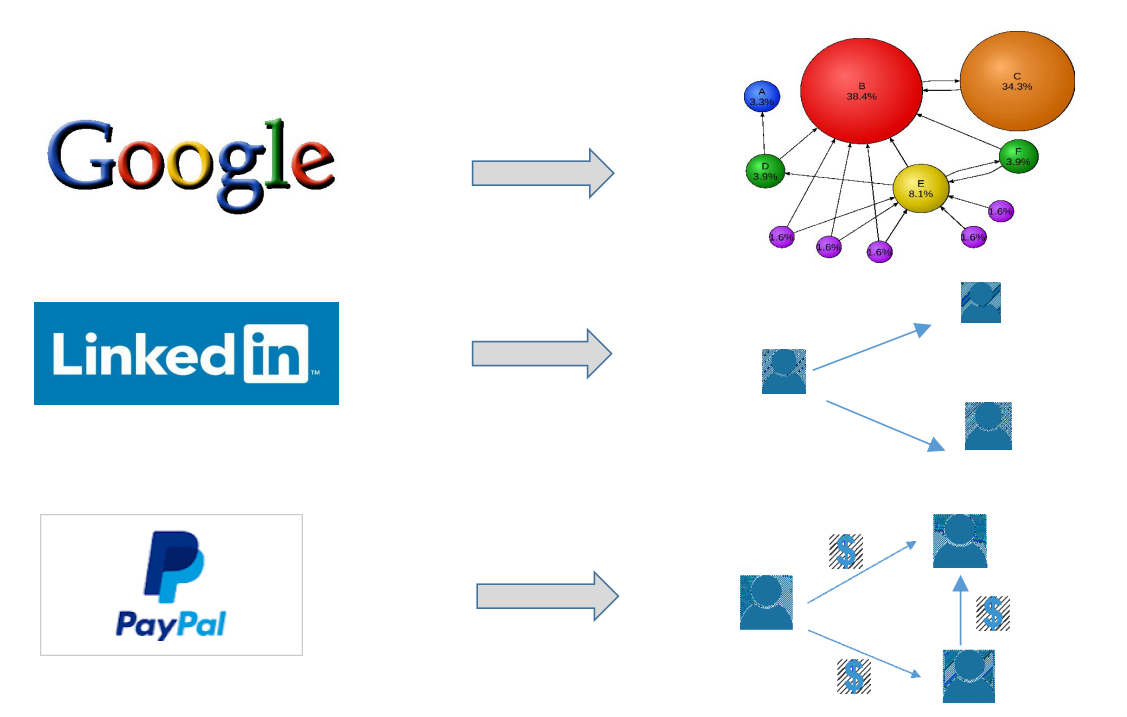
\includegraphics[width=0.8\linewidth,keepaspectratio]{neo4j31}
\end{center}	

{\tiny (Ref: CIS 6930 - Advanced Databases - Neo4j )}
\end{frame}



% \section[Neo4j]{Neo4j}
% %%%%%%%%%%%%%%%%%%%%%%%%%%%%%%%%%%%%%%%%%%%%%%%%%%%%%%%%%%%%%%%%%%%%%%%%%%%%%%%%%%
\begin{frame}[fragile]\frametitle{}
\begin{center}
{\Large Neo4j}
\end{center}
\end{frame}


%%%%%%%%%%%%%%%%%%%%%%%%%%%%%%%%%%%%%%%%%%%%%%%%%%%%%%%%%%%%%%%%%%%%%%%%%%%%%%%%%%
\begin{frame}\frametitle{Introduction}

Neo4j: Network Exploration and Optimization for Java

\begin{itemize}
\item Open Source
\item Implemented in Java and Scala
\item Cypher : mature and rivals SQL
\item ACID (Atomic, Consistent, Isolated, Durable) compliant
\item Embedded Server
\item REST API
\end{itemize}

{\tiny (Ref: CIS 6930 - Advanced Databases - Neo4j )}


\begin{center}
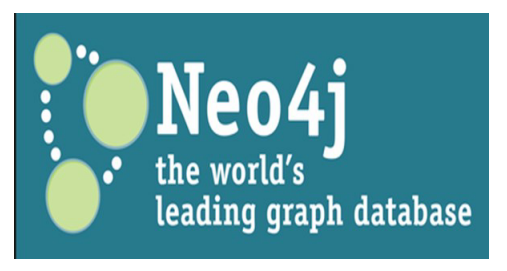
\includegraphics[width=0.6\linewidth,keepaspectratio]{neo4j32}
\end{center}	

\end{frame}


%%%%%%%%%%%%%%%%%%%%%%%%%%%%%%%%%%%%%%%%%%%%%%%%%%%%%%%%%%%
\begin{frame}[fragile]\frametitle{Neo4j}

\begin{center}
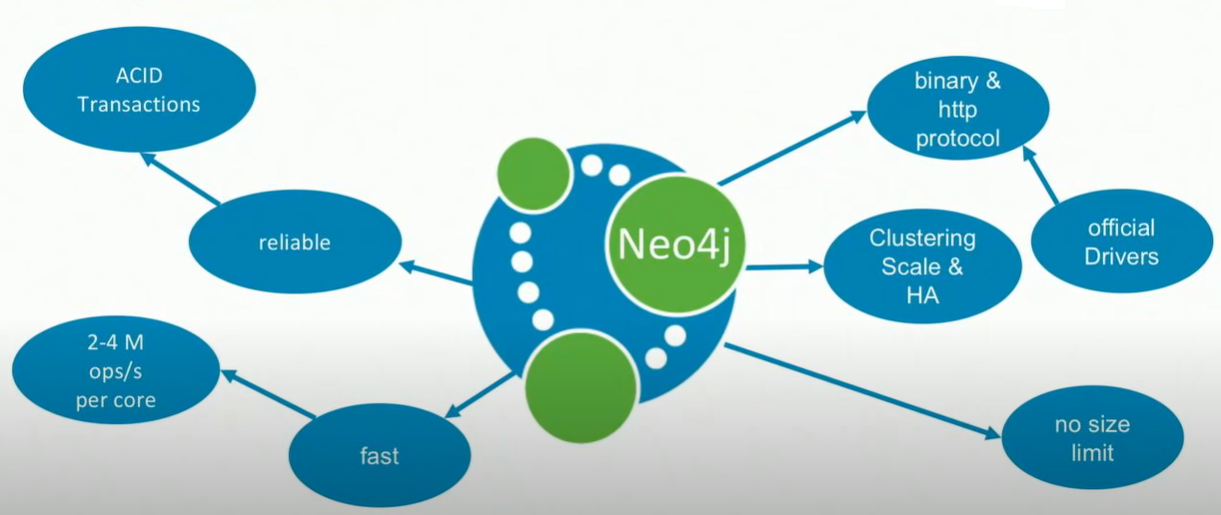
\includegraphics[width=\linewidth,keepaspectratio]{neo4j14}
\end{center}	  

{\tiny (Ref: Introduction to Neo4j and Graph Databases
 - M David Allen)}

\end{frame}

%%%%%%%%%%%%%%%%%%%%%%%%%%%%%%%%%%%%%%%%%%%%%%%%%%%%%%%%%%%%%%%%%%%%%%%%%%%%%%%%%%
\begin{frame}\frametitle{Neo4j features}

\begin{itemize}
\item Capacity: Nodes/Relationships/Labels (all in Billions)
\item High data integrity
\item Native graph processing
\item High scalability
\item Data browser
\end{itemize}

{\tiny (Ref: CIS 6930 - Advanced Databases - Neo4j )}
\end{frame}

%%%%%%%%%%%%%%%%%%%%%%%%%%%%%%%%%%%%%%%%%%%%%%%%%%%%%%%%%%%%%%%%%%%%%%%%%%%%%%%%%%
\begin{frame}\frametitle{Index free adjacency }
With index free adjaceny, when a node or relationship is written to the database, it is stored in the database as connected and any subsequent access to the data is done using pointer navigation which is very fast. Since Neo4j is a native graph database, it supports very large graphs where connected data can be traversed in constant time without the need for an index.

\begin{center}
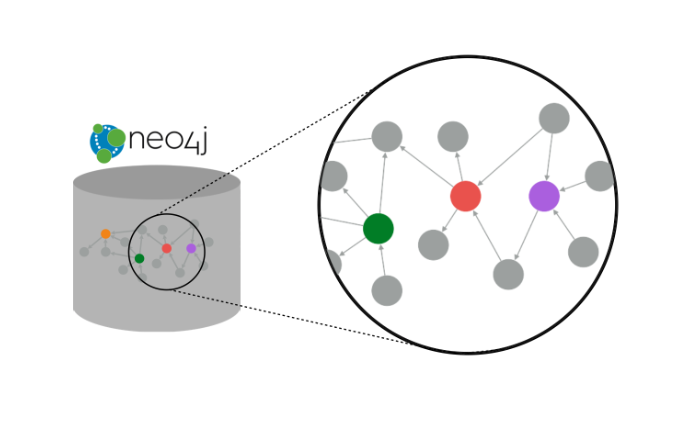
\includegraphics[width=0.6\linewidth,keepaspectratio]{neo4j79}
\end{center}	

{\tiny (Ref: Learning Neo4j - Wabri Github)}
\end{frame}

%%%%%%%%%%%%%%%%%%%%%%%%%%%%%%%%%%%%%%%%%%%%%%%%%%%%%%%%%%%%%%%%%%%%%%%%%%%%%%%%%%
\begin{frame}\frametitle{ACID }
Transactionality is very important for robust applications that require an atomicity, consistency, isolation, and durability guarantees for their data. If a relationship between nodes is created, not only is the relationship created, but the nodes are updated as connected. All of these updates to the database must all succeed or fail.


\begin{center}
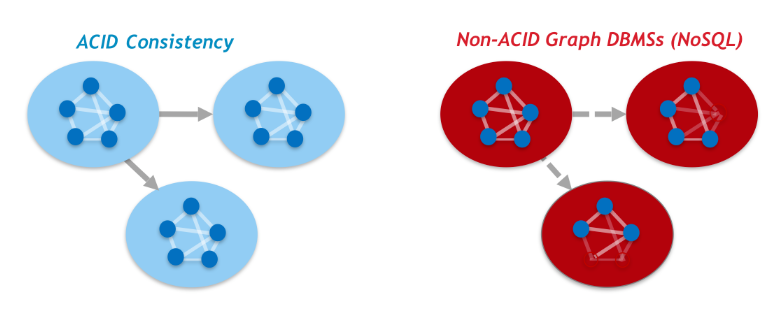
\includegraphics[width=0.8\linewidth,keepaspectratio]{neo4j80}
\end{center}	

{\tiny (Ref: Learning Neo4j - Wabri Github)}
\end{frame}

%%%%%%%%%%%%%%%%%%%%%%%%%%%%%%%%%%%%%%%%%%%%%%%%%%%%%%%%%%%%%%%%%%%%%%%%%%%%%%%%%%
\begin{frame}\frametitle{Clusters }
Neo4j supports clusters that provide high availablity, scalability for read access to the data and failover which is important to many enterprises.

\begin{center}
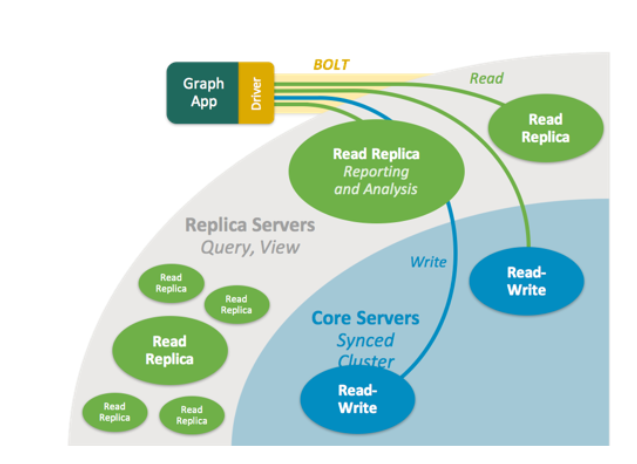
\includegraphics[width=0.6\linewidth,keepaspectratio]{neo4j81}
\end{center}	

{\tiny (Ref: Learning Neo4j - Wabri Github)}
\end{frame}

%%%%%%%%%%%%%%%%%%%%%%%%%%%%%%%%%%%%%%%%%%%%%%%%%%%%%%%%%%%%%%%%%%%%%%%%%%%%%%%%%%
\begin{frame}\frametitle{Misc }

\begin{itemize}
\item The Neo4j graph engine is used to interpret Cypher statements and also executes kernel-level code to store and retrive data, whether it is on disk, or cached in memory.
\item Neo4j supports Java, JavaScript, Python, C\#, and Go drivers that use Neo4j's bolt protocol for binary access to the database layer. Bolt is an efficiant binary protocol that compresses data sent over the wire as well encrypting the data. It's possible to create a java application that uses the bolt driver to access the Neo4j database and the application may use other packages that allow data integration between Neo4j and other data stores or uses as common framework such as spring.
\end{itemize}


{\tiny (Ref: Learning Neo4j - Wabri Github)}
\end{frame}

%%%%%%%%%%%%%%%%%%%%%%%%%%%%%%%%%%%%%%%%%%%%%%%%%%%%%%%%%%%%%%%%%%%%%%%%%%%%%%%%%%
\begin{frame}\frametitle{Tools }

\begin{itemize}
\item Neo4j browser is an application that uses the JavaScript Bolt driver to access the graph engine of the Neo4j database server.
\item Bloom enables you to visualize a graph without knowing much about Cypher (youtube video).
\item  ETL used to importing and exporting data between flat files and a neo4j Database.
\end{itemize}

\begin{center}
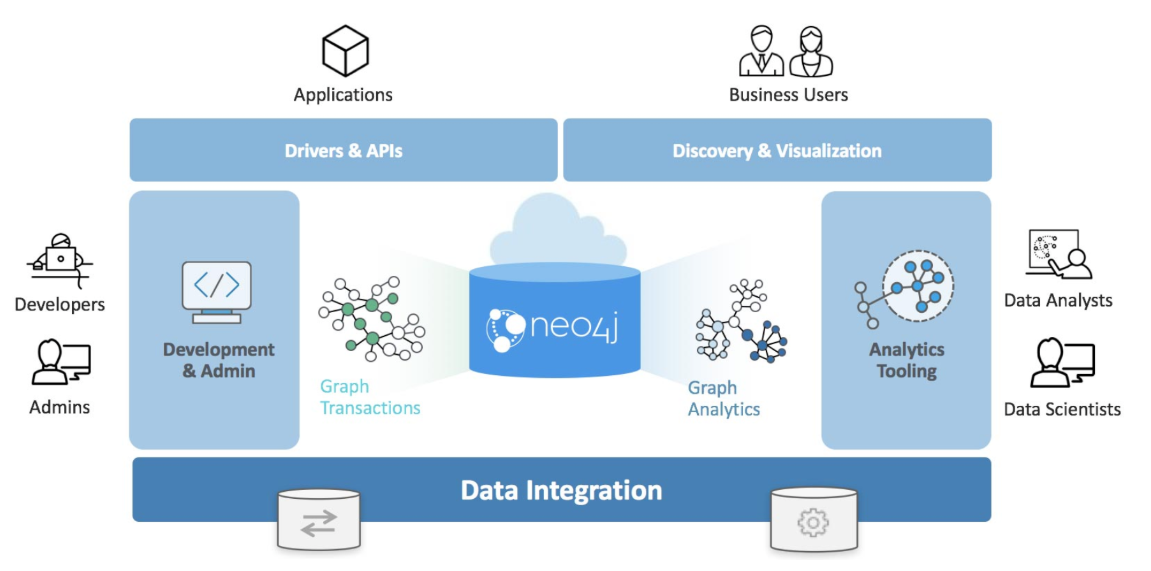
\includegraphics[width=0.8\linewidth,keepaspectratio]{neo4j82}
\end{center}	

{\tiny (Ref: Learning Neo4j - Wabri Github)}
\end{frame}


%%%%%%%%%%%%%%%%%%%%%%%%%%%%%%%%%%%%%%%%%%%%%%%%%%%%%%%%%%%%%%%%%%%%%%%%%%%%%%%%%%
\begin{frame}\frametitle{Usage }

\begin{itemize}
\item Desktop:  Includes the Neo4j Database server which includes the graph engine and kernel so that Cypher statements can be executed to access a database on your system. It includes an application called Neo4j Browser. Neo4j Browser enables you to access a Neo4j database using Cypher. 
\item Browser Sandbox: Is a temporary, cloud-based instance of a Neo4j Server with its associated graph that you can access from any Web browser. The database in a Sandbox may be blank or it may be pre-populated. It is started automatically for you when you create the Sandbox.
\end{itemize}


{\tiny (Ref: Learning Neo4j - Wabri Github)}
\end{frame}


%%%%%%%%%%%%%%%%%%%%%%%%%%%%%%%%%%%%%%%%%%%%%%%%%%%%%%%%%%%%%%%%%%%%%%%%%%%%%%%%%%
\begin{frame}\frametitle{Good For}

\begin{itemize}
\item Highly connected data (social networks)
\item Recommendations (e-commerce)
\item Path Finding (how do I know you?)
\item A* (Least Cost path)
\item  Data First Schema (bottom-up, but you still need to design)
\end{itemize}

{\tiny (Ref: CIntroduction to Graph Databases - Max De Marzi )}
\end{frame}


%%%%%%%%%%%%%%%%%%%%%%%%%%%%%%%%%%%%%%%%%%%%%%%%%%%%%%%%%%%%%%%%%%%%%%%%%%%%%%%%%%
\begin{frame}\frametitle{Property Graph}

\begin{itemize}
\item Labels are node types. There can be multiple labels to a node, e.g. Person, Female, etc.
\item Properties are key-value attributes/fields of node or relationship, e.g. firstname, born.

\end{itemize}
\begin{center}
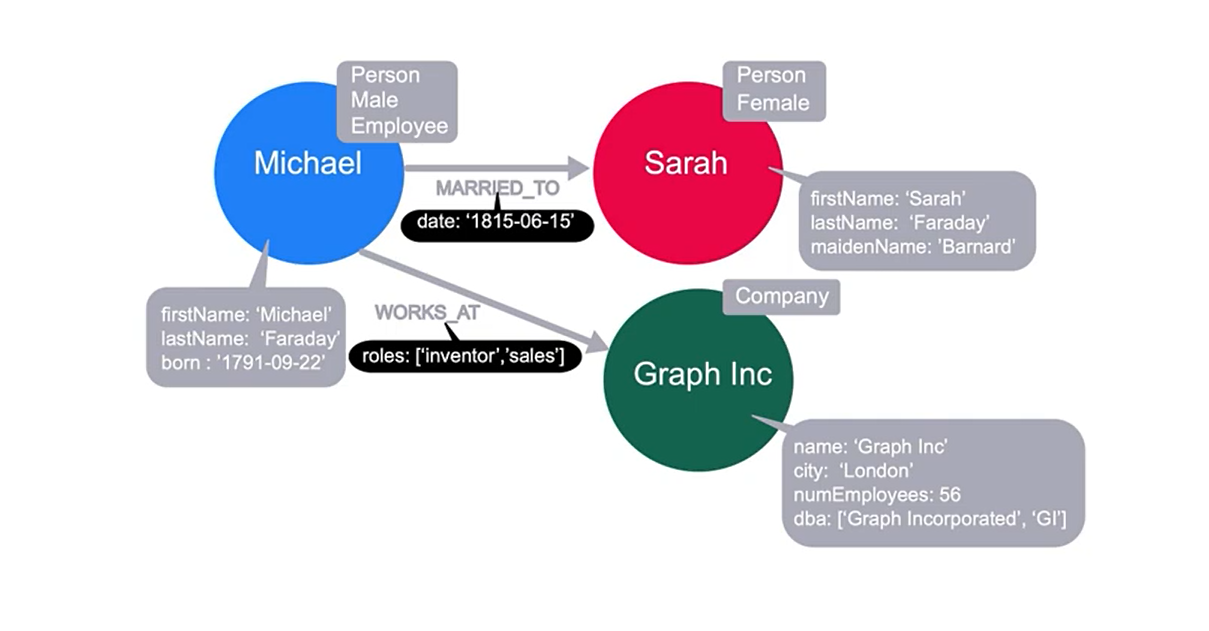
\includegraphics[width=\linewidth,keepaspectratio]{neo4j60}
\end{center}	

{\tiny (Ref: Introduction to Neo4j - a hands-on crash course - neo4j)}
\end{frame}


%%%%%%%%%%%%%%%%%%%%%%%%%%%%%%%%%%%%%%%%%%%%%%%%%%%%%%%%%%%%%%%%%%%%%%%%%%%%%%%%%%
\begin{frame}\frametitle{Property Graph}

\begin{center}
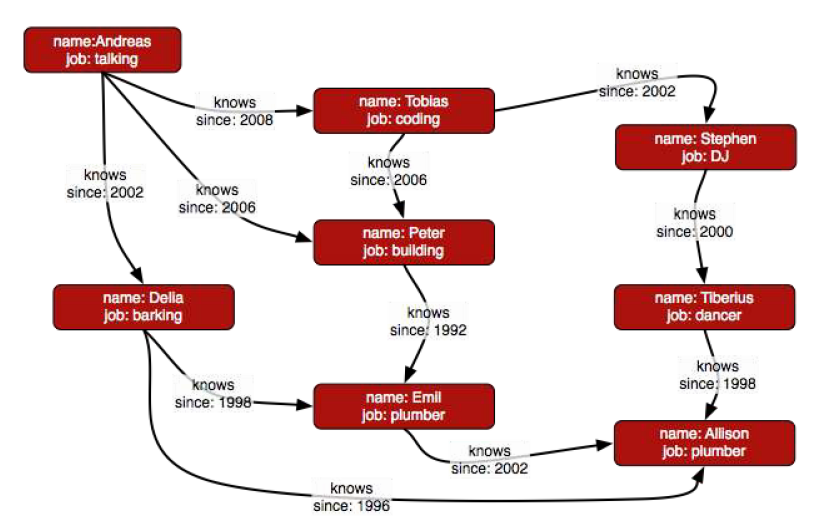
\includegraphics[width=\linewidth,keepaspectratio]{neo4j46}
\end{center}	

{\tiny (Ref: Introduction to Graph Databases - Max De Marzi )}
\end{frame}

%%%%%%%%%%%%%%%%%%%%%%%%%%%%%%%%%%%%%%%%%%%%%%%%%%%%%%%%%%%%%%%%%%%%%%%%%%%%%%%%%%
\begin{frame}\frametitle{Property Graph}

\begin{center}
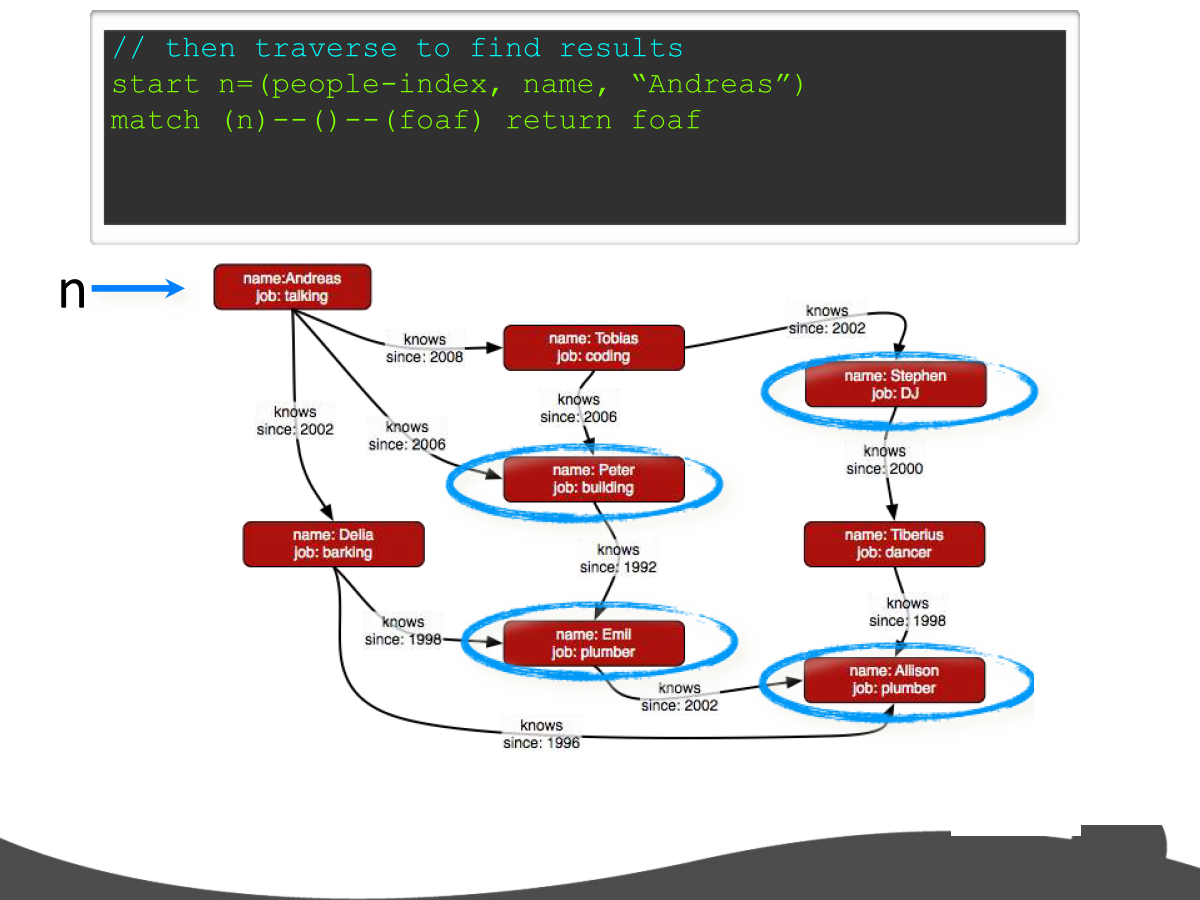
\includegraphics[width=\linewidth,keepaspectratio]{neo4j47}
\end{center}	

{\tiny (Ref: Introduction to Graph Databases - Max De Marzi )}
\end{frame}

%%%%%%%%%%%%%%%%%%%%%%%%%%%%%%%%%%%%%%%%%%%%%%%%%%%%%%%%%%%%%%%%%%%%%%%%%%%%%%%%%%
\begin{frame}\frametitle{Native Graph}

\begin{itemize}
\item Index free adjacency.
\item Each node stores incoming and outgoing relationships.
\item So traversal is from node to node via edges, and not by iterating through linear index.
\end{itemize}

\begin{center}
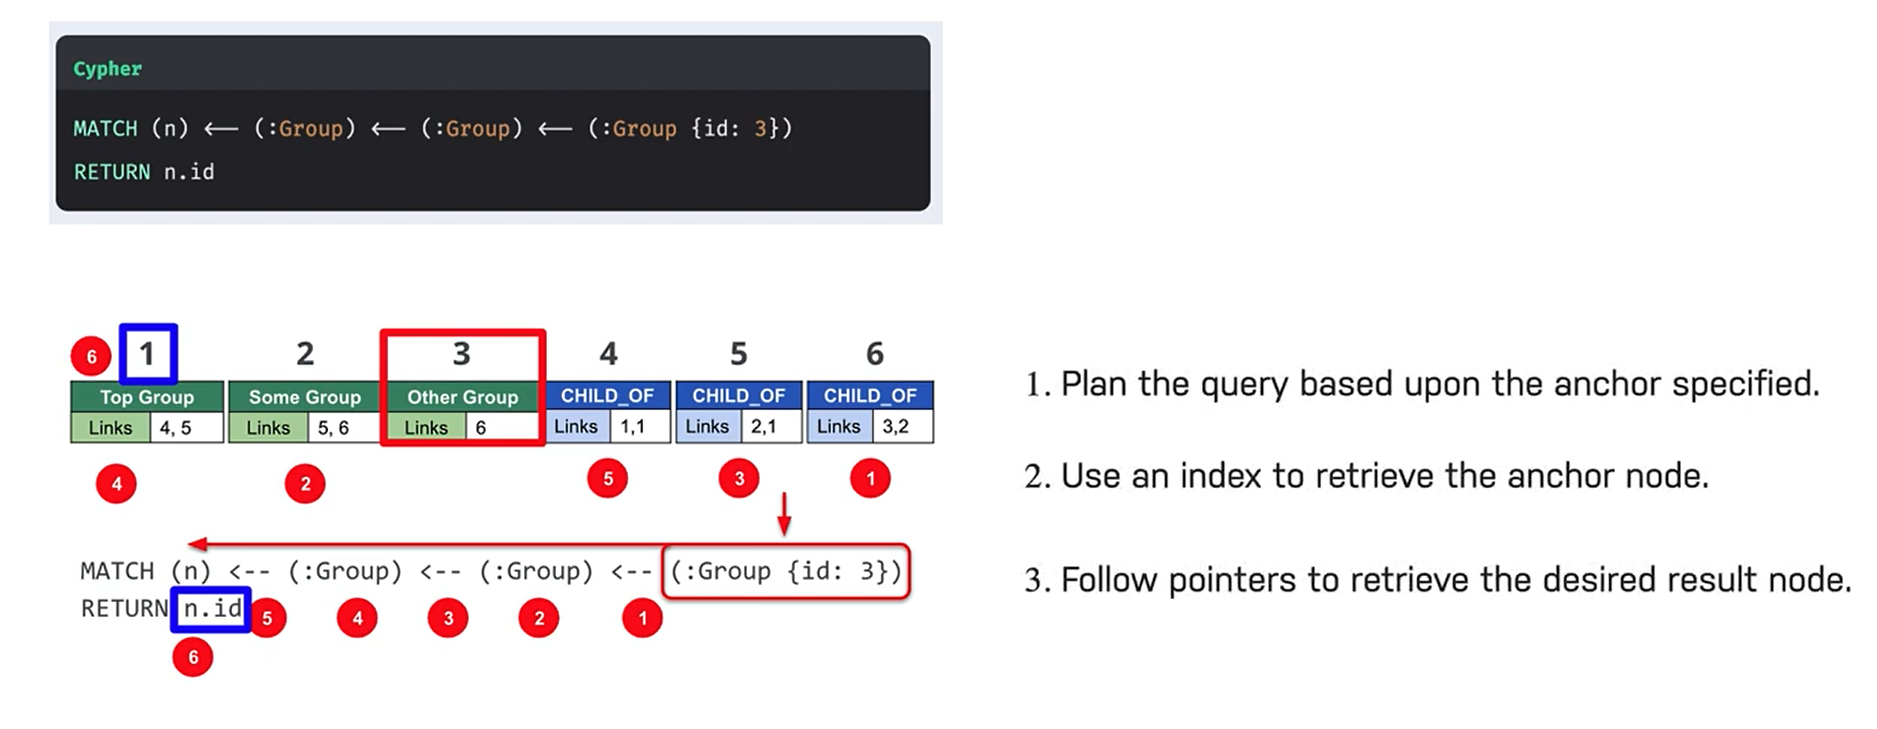
\includegraphics[width=\linewidth,keepaspectratio]{neo4j61}
\end{center}	

{\tiny (Ref: Introduction to Neo4j - a hands-on crash course - neo4j)}
\end{frame}


%%%%%%%%%%%%%%%%%%%%%%%%%%%%%%%%%%%%%%%%%%%%%%%%%%%%%%%%%%%%%%%%%%%%%%%%%%%%%%%%%%
\begin{frame}\frametitle{Cypher}

Pattern Matching Query Language (like SQL for graphs)

\begin{center}
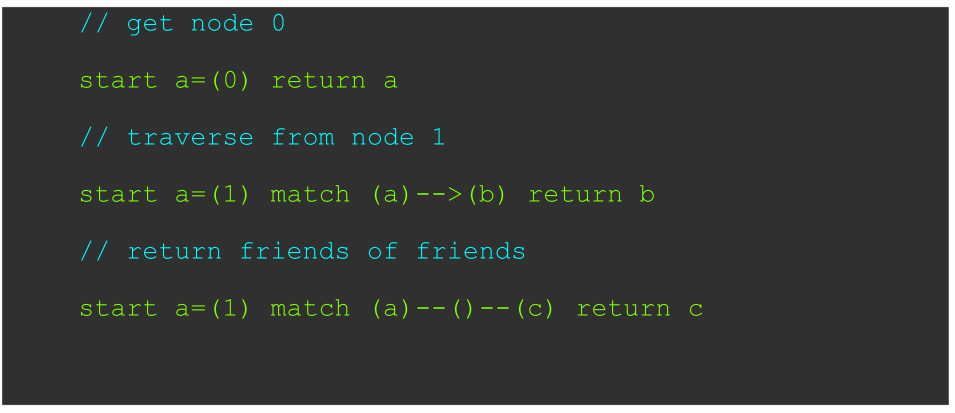
\includegraphics[width=\linewidth,keepaspectratio]{neo4j48}
\end{center}	

{\tiny (Ref: Introduction to Graph Databases - Max De Marzi )}
\end{frame}

%%%%%%%%%%%%%%%%%%%%%%%%%%%%%%%%%%%%%%%%%%%%%%%%%%%%%%%%%%%%%%%%%%%%%%%%%%%%%%%%%%
\begin{frame}\frametitle{Gremlin}

A Graph Scripting DSL (groovy-based)

\begin{center}
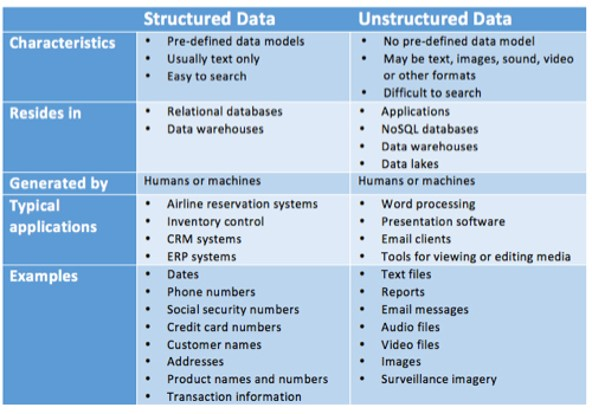
\includegraphics[width=0.8\linewidth,keepaspectratio]{neo4j49}
\end{center}	

{\tiny (Ref: Introduction to Graph Databases - Max De Marzi )}
\end{frame}

%%%%%%%%%%%%%%%%%%%%%%%%%%%%%%%%%%%%%%%%%%%%%%%%%%%%%%%%%%%%%%%%%%%%%%%%%%%%%%%%%%
\begin{frame}\frametitle{If you’ve ever}

\begin{itemize}
\item Joined more than 7 tables together
\item  Modeled a graph in a table
\item  Written a recursive CTE
\item Tried to write some crazy stored procedure with multiple recursive self and inner joins
\end{itemize}

{\bf You should use Neo4j}

{\tiny (Ref: Introduction to Graph Databases - Max De Marzi )}
\end{frame}


%%%%%%%%%%%%%%%%%%%%%%%%%%%%%%%%%%%%%%%%%%%%%%%%%%%%%%%%%%%
\begin{frame}[fragile]\frametitle{Windows Installation}

\begin{itemize}
\item Have Open JDK 11 ready, if not, go to https://learn.microsoft.com/en-us/java/openjdk/download (178 MB)
\item https://neo4j.com/download-center/\#community (4.4.11 129 MB)
\item Place the extracted files in a permanent home on your server, for example \lstinline|D:\neo4j\|. The top level directory is referred to as NEO4J\_HOME.
\item To run Neo4j as a console application, use: \lstinline|<NEO4J_HOME>\bin\neo4j console|

% \begin{lstlisting}
% C:\neo4j\bin>neo4j.bat console
% Directories in use:
% home:         C:\neo4j
% :
% Starting Neo4j.
% \end{lstlisting}

\item Visit http://localhost:7474 in your web browser.
\item Default login is username 'neo4j' and password 'neo4j' Change password. Got conncted to `neo4j://127.0.0.1:7687`
\end{itemize}

(Note: Btw, free, no-download sandbox option is available at sandbox.neo4j.com)
\end{frame}

%%%%%%%%%%%%%%%%%%%%%%%%%%%%%%%%%%%%%%%%%%%%%%%%%%%%%%%%%%%%%%%%%%%%%%%%%%%%%%%%%%
\begin{frame}\frametitle{Neo4j Driver API}


\begin{itemize}
\item  Bolt protocol
\item   Currently supports .NET, Java, JavaScript and Python
\item   Uniformity across languages
\end{itemize}


{\tiny (Ref: CIS 6930 - Advanced Databases - Neo4j )}
\end{frame}

%%%%%%%%%%%%%%%%%%%%%%%%%%%%%%%%%%%%%%%%%%%%%%%%%%%%%%%%%%%%%%%%%%%%%%%%%%%%%%%%%%
\begin{frame}\frametitle{Neo4j Browser}


\begin{itemize}
\item   Developer focused
\item    Export results
\item   Visualization
\end{itemize}

\begin{center}
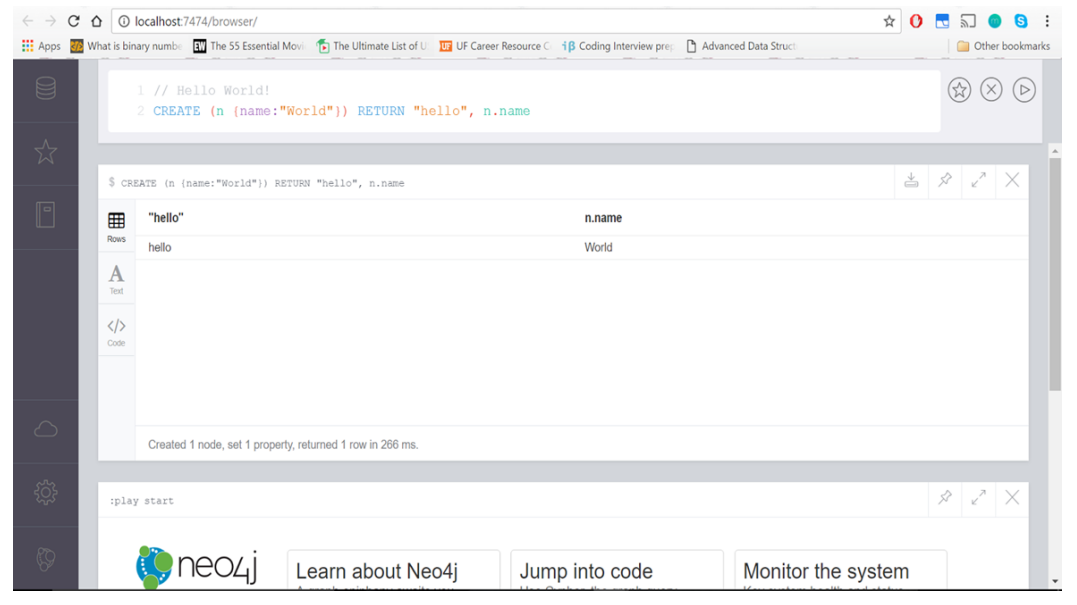
\includegraphics[width=\linewidth,keepaspectratio]{neo4j40}
\end{center}	 

{\tiny (Ref: CIS 6930 - Advanced Databases - Neo4j )}
\end{frame}



%%%%%%%%%%%%%%%%%%%%%%%%%%%%%%%%%%%%%%%%%%%%%%%%%%%%%%%%%%%
\begin{frame}[fragile]\frametitle{Console}

\begin{center}
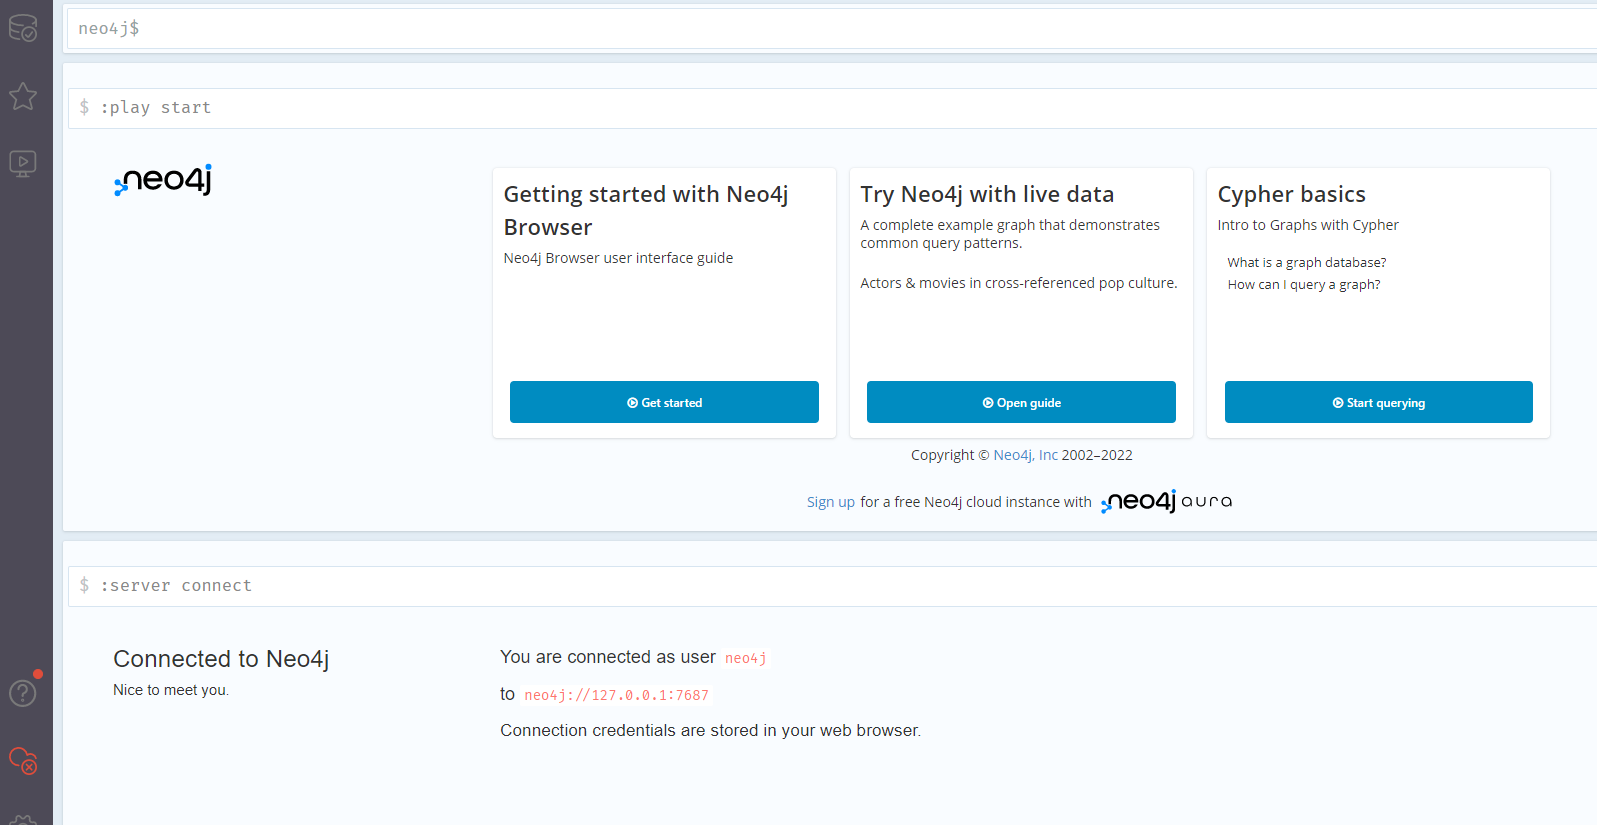
\includegraphics[width=\linewidth,keepaspectratio]{neo4j1}
\end{center}	  


\end{frame}

%%%%%%%%%%%%%%%%%%%%%%%%%%%%%%%%%%%%%%%%%%%%%%%%%%%%%%%%%%%
\begin{frame}[fragile]\frametitle{Interaction}

Type commands in top command window

\begin{itemize}
\item \lstinline|MATCH(n) RETURN n| Return nodes (type none). As there is nothing, nothing gets returned. So create something.
\item \lstinline|CREATE(n)| will create one empty node.
\item \lstinline|MATCH(n) RETURN n| will now return 1 node and show it. $n$ is the reference(s) or the object handle(s), which is returned.
\end{itemize}

\begin{center}
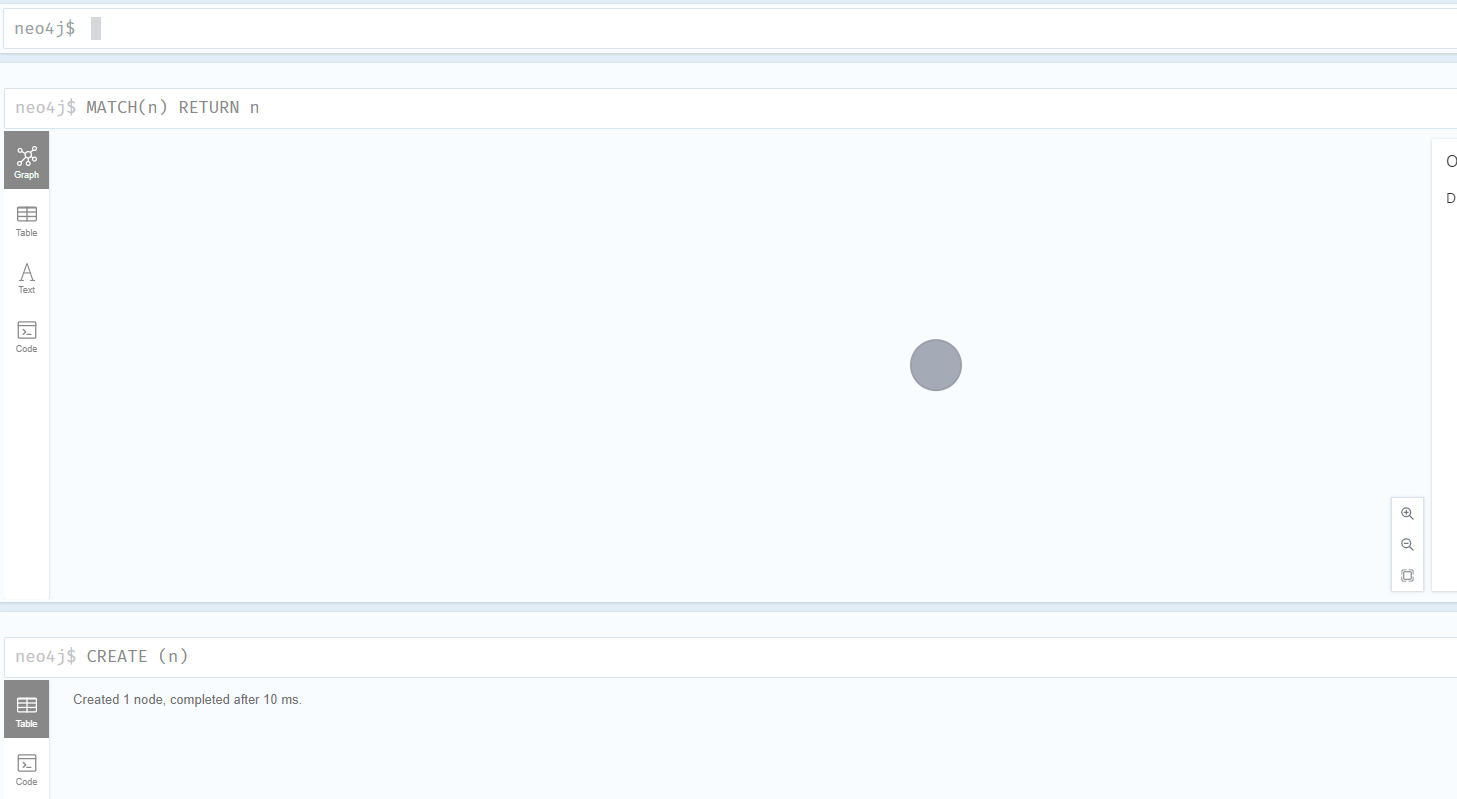
\includegraphics[width=0.8\linewidth,keepaspectratio]{neo4j2}
\end{center}

\end{frame}


%%%%%%%%%%%%%%%%%%%%%%%%%%%%%%%%%%%%%%%%%%%%%%%%%%%%%%%%%%%
\begin{frame}[fragile]\frametitle{Examples}

\begin{itemize}
\item \lstinline|CREATE(n:PERSON)| create a node (type PERSON). Type is actually the label of the node.
\item \lstinline|MATCH(n) DELETE(n)| will delete all the nodes. n, the object handled, returned by MATCH, is getting deleted in the delete function where n is argument. 
\item \lstinline|CREATE(n:PERSON{name:'chris', favoritecolor:'blue'})| create a node (type PERSON) along with some properties. SImilariy, can create different nodes of different type.
\item \lstinline|MATCH(n:PERSON) RETURN n|to selectively return only PERSONs.
\item \lstinline|MATCH(n) RETURN n LIMIT 4| to return only 4 nodes
\item Two create relationship find 2 nodes using \lstinline|MATCH| and \lstinline|WHERE| to restrict, then create relationship 'studied\_at'

\begin{lstlisting}
MATCH (s:School), (p:Person)
WHERE s.name = 'LSU' and p.name = 'jenny'
CREATE (p)-[stu:STUDIED_AT]->(s)
\end{lstlisting}


\end{itemize}

\end{frame}


%%%%%%%%%%%%%%%%%%%%%%%%%%%%%%%%%%%%%%%%%%%%%%%%%%%%%%%%%%%
\begin{frame}[fragile]\frametitle{Examples}


\begin{center}
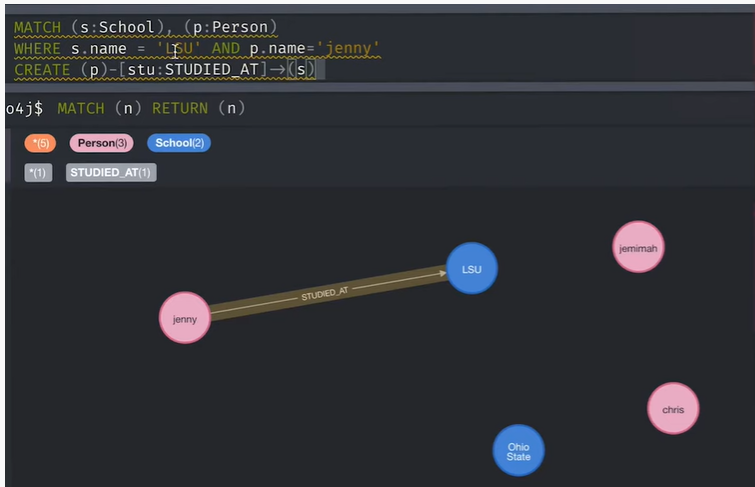
\includegraphics[width=0.9\linewidth,keepaspectratio]{neo4j3}
\end{center}	

{\tiny (Ref: An introduction to neo4j (graph database tutorial for beginners) - Chris Hay)}

\end{frame}

%%%%%%%%%%%%%%%%%%%%%%%%%%%%%%%%%%%%%%%%%%%%%%%%%%%%%%%%%%%
\begin{frame}[fragile]\frametitle{Comparison}
Find all reports and how many people they manage upto 3 levels down.

\begin{center}
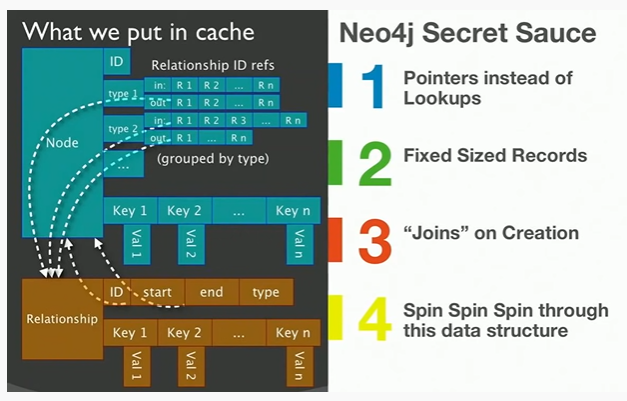
\includegraphics[width=0.8\linewidth,keepaspectratio]{neo4j20}
\end{center}	    

{\tiny (Ref: Introduction to Neo4j and Graph Databases
 - M David Allen)}

\end{frame}

%%%%%%%%%%%%%%%%%%%%%%%%%%%%%%%%%%%%%%%%%%%%%%%%%%%%%%%%%%%
\begin{frame}[fragile]\frametitle{Choice}
When to choose Neo4j over Relational databases? Sub-second response \ldots


\begin{center}
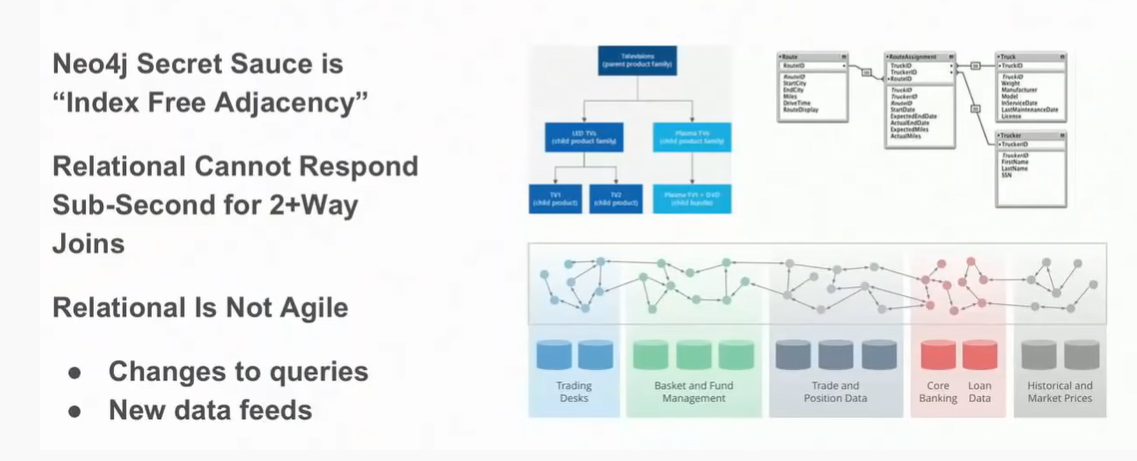
\includegraphics[width=\linewidth,keepaspectratio]{neo4j21}
\end{center}	    

{\tiny (Ref: Introduction to Neo4j and Graph Databases
 - M David Allen)}

\end{frame}


%%%%%%%%%%%%%%%%%%%%%%%%%%%%%%%%%%%%%%%%%%%%%%%%%%%%%%%%%%%
\begin{frame}[fragile]\frametitle{Indexes}
Used only to find the starting points for queries

\begin{center}
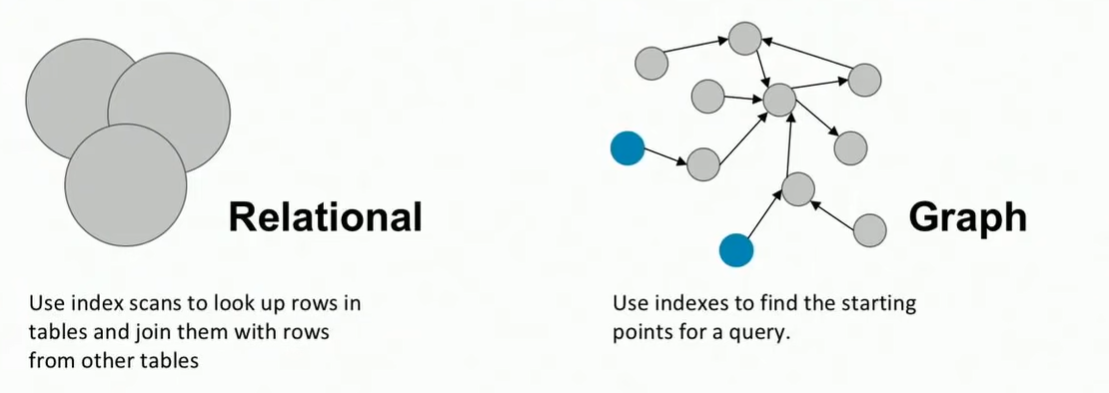
\includegraphics[width=\linewidth,keepaspectratio]{neo4j16}
\end{center}	  


{\tiny (Ref: Introduction to Neo4j and Graph Databases
 - M David Allen)}

\end{frame}

%%%%%%%%%%%%%%%%%%%%%%%%%%%%%%%%%%%%%%%%%%%%%%%%%%%%%%%%%%%%%%%%%%%%%%%%%%%%%%%%%%
\begin{frame}\frametitle{Neo4j Drawbacks}


\begin{itemize}
\item  Scalability
\item   Complex Domains
\item   Complex types
\item   Deleted Records
\end{itemize}

 

{\tiny (Ref: CIS 6930 - Advanced Databases - Neo4j )}
\end{frame}

%%%%%%%%%%%%%%%%%%%%%%%%%%%%%%%%%%%%%%%%%%%%%%%%%%%%%%%%%%%%%%%%%%%%%%%%%%%%%%%%%%
\begin{frame}[fragile]\frametitle{}
\begin{center}
{\Large Architecture}
\end{center}
\end{frame}

%%%%%%%%%%%%%%%%%%%%%%%%%%%%%%%%%%%%%%%%%%%%%%%%%%%%%%%%%%%%%%%%%%%%%%%%%%%%%%%%%%
\begin{frame}\frametitle{Native Graph Processing}



\begin{itemize}
\item Index-free adjacency
\item Each node maintains direct references to its adjacent nodes
\item Efficient query time
\end{itemize}

{\tiny (Ref: CIS 6930 - Advanced Databases - Neo4j )}
\end{frame}

%%%%%%%%%%%%%%%%%%%%%%%%%%%%%%%%%%%%%%%%%%%%%%%%%%%%%%%%%%%%%%%%%%%%%%%%%%%%%%%%%%
\begin{frame}\frametitle{Native Graph Storage}

\begin{center}
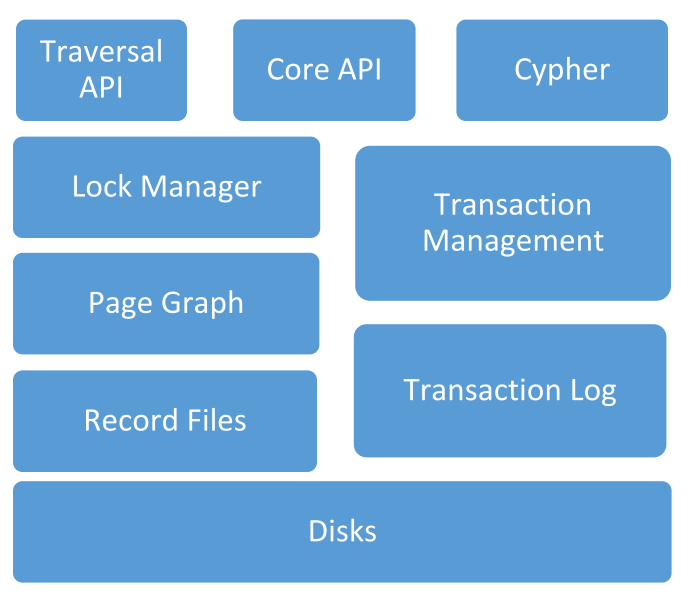
\includegraphics[width=0.5\linewidth,keepaspectratio]{neo4j37}
\end{center}	  


{\tiny (Ref: CIS 6930 - Advanced Databases - Neo4j )}
\end{frame}

%%%%%%%%%%%%%%%%%%%%%%%%%%%%%%%%%%%%%%%%%%%%%%%%%%%%%%%%%%%%%%%%%%%%%%%%%%%%%%%%%%
\begin{frame}\frametitle{Native Graph Storage}

\begin{center}
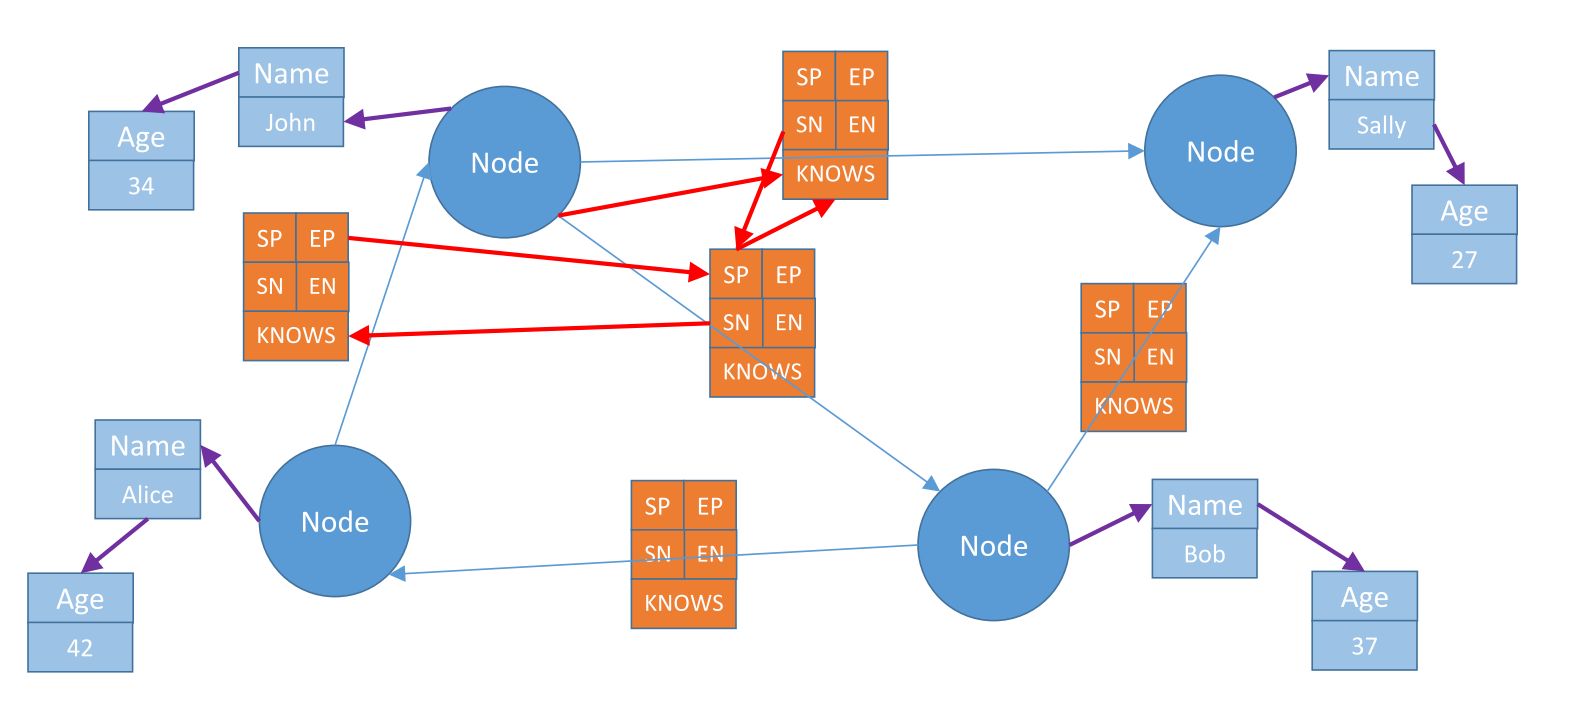
\includegraphics[width=\linewidth,keepaspectratio]{neo4j38}
\end{center}	  


{\tiny (Ref: CIS 6930 - Advanced Databases - Neo4j )}
\end{frame}

%%%%%%%%%%%%%%%%%%%%%%%%%%%%%%%%%%%%%%%%%%%%%%%%%%%%%%%%%%%%%%%%%%%%%%%%%%%%%%%%%%
\begin{frame}\frametitle{Cypher Query Language}

\begin{itemize}
\item Neo4j’s open graph query language
\item Uses patterns to describe graph data
\item Familiar SQL-like clauses
\item Describe what to find, not how to find it
\end{itemize}

{\tiny (Ref: CIS 6930 - Advanced Databases - Neo4j )}
\end{frame}


\section[Query]{Query}
%%%%%%%%%%%%%%%%%%%%%%%%%%%%%%%%%%%%%%%%%%%%%%%%%%%%%%%%%%%%%%%%%%%%%%%%%%%%%%%%%%
\begin{frame}[fragile]\frametitle{}
\begin{center}
{\Large Cypher}
\end{center}
\end{frame}


%%%%%%%%%%%%%%%%%%%%%%%%%%%%%%%%%%%%%%%%%%%%%%%%%%%%%%%%%%%
\begin{frame}[fragile]\frametitle{Introduction}
A pattern matching query language made for graphs

\begin{itemize}
\item Declarative: say, what you want? and not how to search for the answer (Imperative)
\begin{itemize}
\item  Allowing you to focus on your domain instead of getting lost in the syntax of database access.
\item An expressive and efficient queries to handle needed create, read, update, and delete functionality (also know as CRUD operations
\end{itemize}
\item Expressive
\item Pattern-Matching : ASCI Art
\end{itemize}

\end{frame}

%%%%%%%%%%%%%%%%%%%%%%%%%%%%%%%%%%%%%%%%%%%%%%%%%%%%%%%%%%%
\begin{frame}[fragile]\frametitle{Use Case}

Movie Dataset

\begin{itemize}
\item The graph contains nodes with the labels Person and Movie. 
\item Person nodes have several types of relationships to Movie nodes. 
\item A Person node can have a FOLLOWS relationship to another Person node.
\end{itemize}


\begin{center}
\includegraphics[width=0.8\linewidth,keepaspectratio]{neo4j62}
\end{center}	  


{\tiny (Ref: Introduction to cypher fundamentals  - neo4j)}

\end{frame}

%%%%%%%%%%%%%%%%%%%%%%%%%%%%%%%%%%%%%%%%%%%%%%%%%%%%%%%%%%%
\begin{frame}[fragile]\frametitle{Representation}


\begin{itemize}
\item Nodes are represented in round brackets \lstinline|() or (node variable name)|, similar to a circle on witheboard. An anonymous node \lstinline|()| represents one or more nodes during a query processing where there are no restrictions of the type of the node
\item Labels are used as type to group nodes and filter queries against the graph and is defined with a colon \lstinline|(:Label)|. A node can have zero or more labels for example \lstinline|(node), (node:Label), (node:Label1:Label2), (:Label), (:Label1:Label2)|.
\item Relationships are represented as arrow with its label in square bracket in between \lstinline|-[:RELATIONSHIP]->|
\item Aliases or variable names are  used to referred elements to later in the query defined by a name before a name like \lstinline|(node1:Label1)<-[relationship:RELATIONSHIP]-(node2:Label2)| where \lstinline|node1, node2| and \lstinline|relationship| are aliases.
\item he properties of a node are accessed using \lstinline|{variable}.{property_key}|, for example \lstinline|emil.name or movie.title|.
\end{itemize}

{\tiny (Ref: Learning Neo4j - Wabri Github)}


\end{frame}

%%%%%%%%%%%%%%%%%%%%%%%%%%%%%%%%%%%%%%%%%%%%%%%%%%%%%%%%%%%
\begin{frame}[fragile]\frametitle{Representation}


\begin{center}
\includegraphics[width=\linewidth,keepaspectratio]{neo4j63}
\end{center}	  


{\tiny (Ref: Introduction to cypher fundamentals  - neo4j)}

\end{frame}


%%%%%%%%%%%%%%%%%%%%%%%%%%%%%%%%%%%%%%%%%%%%%%%%%%%%%%%%%%%%%%%%%%%%%%%%%%%%%%%%%%
\begin{frame}[fragile]\frametitle{}
\begin{center}
{\Large Reading}
\end{center}
\end{frame}


%%%%%%%%%%%%%%%%%%%%%%%%%%%%%%%%%%%%%%%%%%%%%%%%%%%%%%%%%%%
\begin{frame}[fragile]\frametitle{Basic Syntax}

\begin{center}
\includegraphics[width=\linewidth,keepaspectratio]{neo4j9}
\end{center}	  


{\tiny (Ref: Introduction to Neo4j - a hands-on crash course  - neo4j)}

\end{frame}

%%%%%%%%%%%%%%%%%%%%%%%%%%%%%%%%%%%%%%%%%%%%%%%%%%%%%%%%%%%
\begin{frame}[fragile]\frametitle{Retrieval}


\begin{itemize}
\item Pattern specification for MATCH command, to retrieve data in graph.
\item Find and return person $p$ and movie $m$
\item First finds $p$ with given name, then goes to all relationships with given type and then finds $m$ which matches given title.
\end{itemize}


\begin{center}
\includegraphics[width=0.8\linewidth,keepaspectratio]{neo4j64}
\end{center}	  


{\tiny (Ref: Introduction to cypher fundamentals  - neo4j)}

\end{frame}

%%%%%%%%%%%%%%%%%%%%%%%%%%%%%%%%%%%%%%%%%%%%%%%%%%%%%%%%%%%
\begin{frame}[fragile]\frametitle{Retrieval}

WHERE can be used to add logical expression, which is not possible in MATCH

\begin{center}
\includegraphics[width=0.8\linewidth,keepaspectratio]{neo4j65}
\end{center}	  


{\tiny (Ref: Introduction to cypher fundamentals  - neo4j)}

\end{frame}



%%%%%%%%%%%%%%%%%%%%%%%%%%%%%%%%%%%%%%%%%%%%%%%%%%%%%%%%%%%
\begin{frame}[fragile]\frametitle{MATCH}

Retrieve nodes

\begin{center}
\includegraphics[width=\linewidth,keepaspectratio]{neo4j10}
\end{center}	  


{\tiny (Ref: Introduction to Neo4j - a hands-on crash course  - neo4j)}

\end{frame}

%%%%%%%%%%%%%%%%%%%%%%%%%%%%%%%%%%%%%%%%%%%%%%%%%%%%%%%%%%%
\begin{frame}[fragile]\frametitle{MATCH}

Retrieve nodes with properties

\begin{center}
\includegraphics[width=\linewidth,keepaspectratio]{neo4j11}
\end{center}	  


{\tiny (Ref: Introduction to Neo4j - a hands-on crash course  - neo4j)}

\end{frame}

%%%%%%%%%%%%%%%%%%%%%%%%%%%%%%%%%%%%%%%%%%%%%%%%%%%%%%%%%%%
\begin{frame}[fragile]\frametitle{MATCH}

Retrieve nodes with relationships

\begin{center}
\includegraphics[width=\linewidth,keepaspectratio]{neo4j12}
\end{center}	  


{\tiny (Ref: Introduction to Neo4j - a hands-on crash course  - neo4j)}

\end{frame}

%%%%%%%%%%%%%%%%%%%%%%%%%%%%%%%%%%%%%%%%%%%%%%%%%%%%%%%%%%%
\begin{frame}[fragile]\frametitle{Retrieval}


\begin{itemize}
\item Absence of a property can also be checked in WHERE clause
\item Partial matches are allowed using STARTS\_WITH, ENDS\_WITH keywords
\item String tests are case sensitive, so better to LOWER them.
\item Check presence IN a list
\end{itemize}


\begin{center}
\includegraphics[width=\linewidth,keepaspectratio]{neo4j66}

\includegraphics[width=\linewidth,keepaspectratio]{neo4j67}

\end{center}	  


{\tiny (Ref: Introduction to cypher fundamentals  - neo4j)}

\end{frame}

%%%%%%%%%%%%%%%%%%%%%%%%%%%%%%%%%%%%%%%%%%%%%%%%%%%%%%%%%%%
\begin{frame}[fragile]\frametitle{Aggregates}

No need to specify grouping key. There is no group-by statement. Other Aggregates are SUM, STDDEV, etc.


\begin{lstlisting}
// implicitly groups by p.name
MATCH (p.Person)-[:ACTED_IN]->(m:Movie)
RETURN p.name, count(*) AS numberOfMovies
\end{lstlisting}	  


This function is very useful when you want to count the number of occurrences of a particular query result. It's possible to specify the occurrences of an alias count(n) and the graph engine calculates the number of occurrences of n. If we want to calculates the number of rows retrieved, including those with null values the count argument need to be a *. Last one is the count() without argument and this will implicit group by based upon the aggregation.

{\tiny (Ref: Learning Neo4j - Wabri Github)}

\end{frame}

%%%%%%%%%%%%%%%%%%%%%%%%%%%%%%%%%%%%%%%%%%%%%%%%%%%%%%%%%%%%%%%%%%%%%%%%%%%%%%%%%%
\begin{frame}\frametitle{Properties }

\begin{itemize}
\item Properties can be used to filter queries so that a subset of the graph is retrieved. \lstinline|CALL db.propertyKeys|
\item Nodes properties filtering \lstinline|MATCH (variable:Label {propertyKey1: propertyValue1, propertyKey2: propertyValue2}) RETURN variable|
\item In addition, with the RETURN clause, you can return property values from the retrieved nodes, rather than the nodes. \lstinline|MATCH (variable {property1: value}) RETURN variable.property2|
\end{itemize}


{\tiny (Ref: Learning Neo4j - Wabri Github)}
\end{frame}

% %%%%%%%%%%%%%%%%%%%%%%%%%%%%%%%%%%%%%%%%%%%%%%%%%%%%%%%%%%%%%%%%%%%%%%%%%%%%%%%%%%
% \begin{frame}\frametitle{Aliases }

% \begin{itemize}
% \item To customize the headings for a table containing property value it can be use aliases: \lstinline|MATCH variable:Label {property1: value, property2: value}) RETURN variable.property2 AS alias1, variable.property3 AS alias2|
% \item In the graph database we can specify aliases for the returned property values: \lstinline|MATCH (p:Person {born: 1970}) RETURN p.name AS name, p.born AS `birth year`|
% \end{itemize}


% {\tiny (Ref: Learning Neo4j - Wabri Github)}
% \end{frame}

% %%%%%%%%%%%%%%%%%%%%%%%%%%%%%%%%%%%%%%%%%%%%%%%%%%%%%%%%%%%%%%%%%%%%%%%%%%%%%%%%%%
% \begin{frame}\frametitle{Relationships}

% The relationship can be specified with or without direction.

% \begin{lstlisting}
% () // a node
% ()--() // 2 nodes have some type of relationship
% ()-->() // the first node has a relationship to the second node
% ()<--() // the second node has a relationship to the first node 
% \end{lstlisting}

% {\tiny (Ref: Learning Neo4j - Wabri Github)}
% \end{frame}

% %%%%%%%%%%%%%%%%%%%%%%%%%%%%%%%%%%%%%%%%%%%%%%%%%%%%%%%%%%%%%%%%%%%%%%%%%%%%%%%%%%
% \begin{frame}\frametitle{Style recommendations}

% \begin{itemize}
% \item Node labels are CamelCase and begin with an upper-case letter, like Person or NetworkAddress.
% \item Property keys, variables, parameters, aliases, and functions are camelCase and begin with a lower-case letter, like title or businessAddress.
% \item Relationship type are in upper-case and can use the underscore, like ACTED\_IN or FOLLOWS.
% \item Cypher keywords are upper-case, like MATCH or RETURN.
% \item String constants are in single quotes, unless the string contains a quote or apostrophe, like 'The Matrix' or ``Somethings Gotta Give''.
% \item Specify variables only when needed for use later in the cypher statement.
% \item Place named nodes and relationships before anonymous nodes and relationships in the MATCH clauses when possible.
% \item Specify anonymous relationships with \lstinline|-->, --, or <--|
% \end{itemize}

% {\tiny (Ref: Learning Neo4j - Wabri Github)}
% \end{frame}

% %%%%%%%%%%%%%%%%%%%%%%%%%%%%%%%%%%%%%%%%%%%%%%%%%%%%%%%%%%%%%%%%%%%%%%%%%%%%%%%%%%
% \begin{frame}\frametitle{Multiple Match patterns}

% The MATCH clause includes a pattern specified by two paths separated by a comma:



% \begin{lstlisting}
% MATCH (a:Person)-[:ACTED_IN]->(m:Movie),
    % (m:Movie)<-[:DIRECTED]-(d:Person)
% WHERE m.released = 2000
% RETURN a.name, m.title, d.name
% \end{lstlisting}

% {\tiny (Ref: Learning Neo4j - Wabri Github)}
% \end{frame}

% %%%%%%%%%%%%%%%%%%%%%%%%%%%%%%%%%%%%%%%%%%%%%%%%%%%%%%%%%%%%%%%%%%%%%%%%%%%%%%%%%%
% \begin{frame}\frametitle{Setting path variables}

% It's possible to assign to a variable a path that can be reuse later in the same query or if it's needed to return that path:


% \begin{lstlisting}
% MATCH megPath = (meg:Person)-[:ACTED_IN]->(m:Movie)<-[:DIRECTED]-(d:Person),
    % (other:Person)-[:ACTED_IN]->(m)
% WHERE meg.name = 'Meg Ryan'
% RETURN megPath
% \end{lstlisting}

% {\tiny (Ref: Learning Neo4j - Wabri Github)}
% \end{frame}

% %%%%%%%%%%%%%%%%%%%%%%%%%%%%%%%%%%%%%%%%%%%%%%%%%%%%%%%%%%%%%%%%%%%%%%%%%%%%%%%%%%
% \begin{frame}\frametitle{Varying length paths}

% It's possible to assign to a variable a path that can be reuse later in the same query or if it's needed to return that path:


% \begin{itemize}
% \item Any graph that represents social networking, trees, or hierarchies will most likely have multiple paths of varying lengths.

% \item To get this far you need to use this format \lstinline|(nodeA)-[:REALTYPE*<number_of_hops>]->(nodeB) or (nodeA)-[:REALTYPE*n..m]->(nodeB)| where n and m are the extremes of an interval.
% \end{itemize}

% {\tiny (Ref: Learning Neo4j - Wabri Github)}
% \end{frame}

% %%%%%%%%%%%%%%%%%%%%%%%%%%%%%%%%%%%%%%%%%%%%%%%%%%%%%%%%%%%%%%%%%%%%%%%%%%%%%%%%%%
% \begin{frame}\frametitle{Finding the shortest path}

% A built-in function that you may find useful in a graph that has many ways of traversing the graph to get to the same node is the shortestPath() function. Using the shortest path between two nodes improves the performance of the query.

% \begin{lstlisting}
% MATCH p = shortestPath((m1:Movie)-[*]-(m2:Movie))
% WHERE m1.title = 'A Few Good Men' AND
    % m2.title = 'The Matrix'
% RETURN p
% \end{lstlisting}

% {\tiny (Ref: Learning Neo4j - Wabri Github)}
% \end{frame}

% %%%%%%%%%%%%%%%%%%%%%%%%%%%%%%%%%%%%%%%%%%%%%%%%%%%%%%%%%%%%%%%%%%%%%%%%%%%%%%%%%%
% \begin{frame}\frametitle{Optional pattern matching}
% This clause OPTIONAL MATCH is just like the MATCH but if no matches are found, this clause will use null for missing parts of the pattern. Here is an examples:

% \begin{lstlisting}
% MATCH (p:Person)
% WHERE p.name STARTS WITH 'James'
% OPTIONAL MATCH (p)-[r:REVIEWED]->(m:Movie)
% RETURN p.name, type(r), m.title
% \end{lstlisting}

% The return will be a table like this:

% \begin{center}
% \includegraphics[width=0.4\linewidth,keepaspectratio]{neo4j83}
% \end{center}	


% {\tiny (Ref: Learning Neo4j - Wabri Github)}
% \end{frame}

% %%%%%%%%%%%%%%%%%%%%%%%%%%%%%%%%%%%%%%%%%%%%%%%%%%%%%%%%%%%%%%%%%%%%%%%%%%%%%%%%%%
% \begin{frame}\frametitle{Collecting results }

% Cypher has a built-in function collect() that enables you to aggregate value into a list:



% \begin{lstlisting}
% MATCH (p:Person)-[:ACTED_IN]->(m:Movie)
% WHERE p.name = 'Tom Cruise'
% RETURN collect(m.title) AS `movies for Tom Cruise`
% \end{lstlisting}

% And the result will be a list called movies for Tom Cruise with the values ["Jerry Maguire", "Top Gun", "A Few Good Men"].


% {\tiny (Ref: Learning Neo4j - Wabri Github)}
% \end{frame}

% %%%%%%%%%%%%%%%%%%%%%%%%%%%%%%%%%%%%%%%%%%%%%%%%%%%%%%%%%%%%%%%%%%%%%%%%%%%%%%%%%%
% \begin{frame}\frametitle{Additional processing using WITH}

% During the execution of a MATCH clause, is possible to specify some intermediate calculations or values that will be used for further processing of the query, or for limiting the number of results before further processing is done. With the WITH clause it's possible to perform intermediate processing of data flow operations.


% \begin{lstlisting}
% MATCH (a:Person)-[:ACTED_IN]->(m:Movie)
% WITH a, count(a) AS numMovies, collect(m.title) AS movies
% WHERE numMovies > 1 AND numMovies < 4
% RETURN a.name, numMovies, movies
% \end{lstlisting}

% This example return the actors name only if they acted on 2 or 3 movies, with a reference of the numbers of the films and a list of that.

% Be carefull with this clause because in the WITH body are specify some variables from the previous part of the query that need to be part of the next section of the query, all the aliases for the next part are the only one defined in the body.


% {\tiny (Ref: Learning Neo4j - Wabri Github)}
% \end{frame}

% %%%%%%%%%%%%%%%%%%%%%%%%%%%%%%%%%%%%%%%%%%%%%%%%%%%%%%%%%%%%%%%%%%%%%%%%%%%%%%%%%%
% \begin{frame}\frametitle{Additional processing using WITH}

% Remember to name all expressions with an alias in a WITH that are not simple variables.

% \begin{lstlisting}
% MATCH (p:Person)
% WITH p, size((p)-[:ACTED_IN]->(:Movie)) as movies
% WHERE movies>=5
% OPTIONAL MATCH (p)-[:DIRECTED]->(m:Movie)
% RETURN p.name, m.title
% \end{lstlisting}

% This is a simple query to retrive all the actor that are acted in at least 5 movies and if they also directed a movie than return the name of that movie.

% \begin{center}
% \includegraphics[width=0.4\linewidth,keepaspectratio]{neo4j84}
% \end{center}	


% {\tiny (Ref: Learning Neo4j - Wabri Github)}
% \end{frame}

% %%%%%%%%%%%%%%%%%%%%%%%%%%%%%%%%%%%%%%%%%%%%%%%%%%%%%%%%%%%%%%%%%%%%%%%%%%%%%%%%%%
% \begin{frame}\frametitle{Eliminating duplication}

% To eliminating duplicated results it can be used the DISTINCT keyword



% \begin{lstlisting}
% MATCH (gene:Person)-[:ACTED_IN]->(movie:Movie)
% WHERE gene.name = 'Gene Hackman'
% OPTIONAL MATCH
    % (other:Person)-[:ACTED_IN]->(movie),
    % (dir:Person)-[:DIRECTED]->(movie)
% WITH
    % movie,
    % collect(other.name) AS Actors,
    % collect(DISTINCT dir.name) AS Directors
% RETURN
    % movie.title AS `Title of movie`,
    % Actors AS `Co-Actors`,
    % Directors
% \end{lstlisting}

% This clause can be use in several uses, like this:


% \begin{lstlisting}
% MATCH (p:Person)-[:DIRECTED | :ACTED_IN]->(m:Movie)
% WHERE p.name = 'Tom Hanks'
% WITH DISTINCT m
% RETURN m.released, m.title
% \end{lstlisting}

% {\tiny (Ref: Learning Neo4j - Wabri Github)}
% \end{frame}

% %%%%%%%%%%%%%%%%%%%%%%%%%%%%%%%%%%%%%%%%%%%%%%%%%%%%%%%%%%%%%%%%%%%%%%%%%%%%%%%%%%
% \begin{frame}\frametitle{Ordering result}

% If you want the results to be sorted, you specify the expression to use for the sort usign the ORDER BY keyword and whether you want the order to be descending using the DESC keyword.


% \begin{lstlisting}
% MATCH (p:Person)-[:DIRECTED | :ACTED_IN]->(m:Movie)
% WHERE p.name = 'Tom Hanks' AND m.released >= 2000
% RETURN m.released, collect(DISTINCT m.title) AS movies ORDER BY m.released DESC
% \end{lstlisting}

% \begin{center}
% \includegraphics[width=\linewidth,keepaspectratio]{neo4j85}
% \end{center}	  


% {\tiny (Ref: Learning Neo4j - Wabri Github)}
% \end{frame}

% %%%%%%%%%%%%%%%%%%%%%%%%%%%%%%%%%%%%%%%%%%%%%%%%%%%%%%%%%%%%%%%%%%%%%%%%%%%%%%%%%%
% \begin{frame}\frametitle{Limiting the number of results}

% Although you can filter queries to reduce the number of results returned, you may also want to limit the number of results. This is useful if you have very large result sets and you only need to see the beginning or end of a set of ordered results. LIMIT is the right choice to do something like this.

% \begin{lstlisting}
% MATCH (m:Movie)
% RETURN m.title as title, m.released as year
% ORDER BY m.released DESC
% LIMIT 10
% \end{lstlisting}


% {\tiny (Ref: Learning Neo4j - Wabri Github)}
% \end{frame}


% %%%%%%%%%%%%%%%%%%%%%%%%%%%%%%%%%%%%%%%%%%%%%%%%%%%%%%%%%%%%%%%%%%%%%%%%%%%%%%%%%%
% \begin{frame}\frametitle{List}

% A Cypher map is list of key/value pairs where each element of the list is of the format key: value.

% It's possible to collect values for a list during a query and with this it's possible to sort by the size of the list using the size() function as follows:

% \begin{lstlisting}
% MATCH (a:Person)-[:ACTED_IN]->(m:Movie)
% WITH m, count(m) AS numCast, collect(a.name) AS cast
% RETURN m.title, cast, numCast
% ORDER BY size(cast)
% \end{lstlisting}


% {\tiny (Ref: Learning Neo4j - Wabri Github)}
% \end{frame}



% %%%%%%%%%%%%%%%%%%%%%%%%%%%%%%%%%%%%%%%%%%%%%%%%%%%%%%%%%%%%%%%%%%%%%%%%%%%%%%%%%%
% \begin{frame}\frametitle{Unwinding lists}

% There my be some situations where you want to perform the opposite of collecting results, but rather separate the lists into separate rows. This functionality is done using the unwind clause.

% Here is an example where we create a list with three elements, unwind the list and then return the values. Since there are three elements, three rows are returned with the values:

% \begin{lstlisting}
% WITH [1, 2, 3] AS list
% UNWIND list AS row
% RETURN row, list
% \end{lstlisting}

% and the result will be:

% \begin{center}
% \includegraphics[width=0.3\linewidth,keepaspectratio]{neo4j86}
% \end{center}	 

% The unwind clause is frequently used when importing data into a graph.

 

% {\tiny (Ref: Learning Neo4j - Wabri Github)}
% \end{frame}

% %%%%%%%%%%%%%%%%%%%%%%%%%%%%%%%%%%%%%%%%%%%%%%%%%%%%%%%%%%%%%%%%%%%%%%%%%%%%%%%%%%
% \begin{frame}\frametitle{Dates}

% Cypher has a built-in date() function, as well as other temporal values and functions that you can use to calculate temporal values. You use a combination of numeric, temporal, spatial, list and string functions to calculate values that are useful to your application.

% For example we want to calculate all the age value of the actors given the born year:

% \begin{lstlisting}
% MATCH (actor:Person)-[:ACTED_IN]->(:Movie)
% WHERE exists(actor.born)
% WITH DISTINCT actor, date().year - actor.born AS age
% RETURN actor.name, age AS `age today`
% ORDER BY actor.born DESC
% \end{lstlisting}



% {\tiny (Ref: Learning Neo4j - Wabri Github)}
% \end{frame}



% %%%%%%%%%%%%%%%%%%%%%%%%%%%%%%%%%%%%%%%%%%%%%%%%%%%%%%%%%%%
% \begin{frame}[fragile]\frametitle{Complex Example}
% A Social Recommendation

% \begin{center}
% \includegraphics[width=\linewidth,keepaspectratio]{neo4j15}
% \end{center}	  


% {\tiny (Ref: Introduction to Neo4j and Graph Databases
 % - M David Allen)}

% \end{frame}



% %%%%%%%%%%%%%%%%%%%%%%%%%%%%%%%%%%%%%%%%%%%%%%%%%%%%%%%%%%%
% \begin{frame}[fragile]\frametitle{Complex Example}
% What are the top 10 jobs for me, that are same location as I am in and also for which I have necessary qualifications?

% \begin{center}
% \includegraphics[width=\linewidth,keepaspectratio]{neo4j27}
% \end{center}	    



% {\tiny (Ref: Secret Sauce of Neo4j: Modeling and Querying Graphs
 % - Max De Marzi )}

% \end{frame}

% %%%%%%%%%%%%%%%%%%%%%%%%%%%%%%%%%%%%%%%%%%%%%%%%%%%%%%%%%%%
% \begin{frame}[fragile]\frametitle{Answer}

% Partial sub-graph match

% \begin{center}
% \includegraphics[width=\linewidth,keepaspectratio]{neo4j28}
% \end{center}	    


% {\tiny (Ref: Secret Sauce of Neo4j: Modeling and Querying Graphs
 % - Max De Marzi )}

% \end{frame}

% %%%%%%%%%%%%%%%%%%%%%%%%%%%%%%%%%%%%%%%%%%%%%%%%%%%%%%%%%%%%%%%%%%%%%%%%%%%%%%%%%%
% \begin{frame}[fragile]\frametitle{}
% \begin{center}
% {\Large Writing}
% \end{center}
% \end{frame}



% %%%%%%%%%%%%%%%%%%%%%%%%%%%%%%%%%%%%%%%%%%%%%%%%%%%%%%%%%%%
% \begin{frame}[fragile]\frametitle{Nodes}

% \begin{itemize}
% \item MERGE: Creates a new node if not present already. All subsequent calls do not do anything as node with said properties is already present.

% \item CREATE: Will create multiple nodes even if nodes with similar properties are present already
% \end{itemize}

% \begin{center}
% \includegraphics[width=0.5\linewidth,keepaspectratio]{neo4j68}
% \end{center}	  


% {\tiny (Ref: Introduction to cypher fundamentals  - neo4j)}

% \end{frame}

% %%%%%%%%%%%%%%%%%%%%%%%%%%%%%%%%%%%%%%%%%%%%%%%%%%%%%%%%%%%
% \begin{frame}[fragile]\frametitle{Nodes}


% \begin{center}
% \includegraphics[width=\linewidth,keepaspectratio]{neo4j13}
% \end{center}	  


% {\tiny (Ref: Introduction to Neo4j - a hands-on crash course  - neo4j)}

% \end{frame}


% %%%%%%%%%%%%%%%%%%%%%%%%%%%%%%%%%%%%%%%%%%%%%%%%%%%%%%%%%%%
% \begin{frame}[fragile]\frametitle{Relationships}

% \begin{itemize}
% \item First get two existing nodes between which a relationship needs to be created.
% \item Same MERGE logic is there for Relationships as well.
% item Relationship type must begin with ':'
% \end{itemize}

% \begin{center}
% \includegraphics[width=0.8\linewidth,keepaspectratio]{neo4j69}
% \end{center}	  


% {\tiny (Ref: Introduction to cypher fundamentals  - neo4j)}

% \end{frame}

% %%%%%%%%%%%%%%%%%%%%%%%%%%%%%%%%%%%%%%%%%%%%%%%%%%%%%%%%%%%
% \begin{frame}[fragile]\frametitle{Properties}

% \begin{itemize}
% \item Use SET to set new or existing properties
% \item It can be used for both Nodes and Relationships
% \item Use REMOVE to remove a property. (it should not be a primary key though)
% \end{itemize}

% \begin{center}
% \includegraphics[width=0.5\linewidth,keepaspectratio]{neo4j70}
% \end{center}	  


% {\tiny (Ref: Introduction to cypher fundamentals  - neo4j)}

% \end{frame}


% %%%%%%%%%%%%%%%%%%%%%%%%%%%%%%%%%%%%%%%%%%%%%%%%%%%%%%%%%%%
% \begin{frame}[fragile]\frametitle{Constrains}
% We add a uniqueness constraint to the graph by creating a constraint that asserts that a particular node property is unique in the graph for a particular type of node.

% \begin{lstlisting}
% // to ensure uniqueness and fast lookups
% CREATE CONSTRAINT ON (label:Label)
% ASSERT label.property IS UNIQUE
% \end{lstlisting}	  

% This statement will fail if the graph already has multiple Movie nodes with the same value for the title property.

% We can also create a constraint on properties of relationships, it's not necessary to define the direction of the relationship:

% \begin{lstlisting}
% CREATE CONSTRAINT ON ()-[rel:REVIEWED]-() ASSERT exists(rel.rating)
% \end{lstlisting}	  

% {\tiny (Ref: Learning Neo4j - Wabri Github)}

% \end{frame}

% %%%%%%%%%%%%%%%%%%%%%%%%%%%%%%%%%%%%%%%%%%%%%%%%%%%%%%%%%%%
% \begin{frame}[fragile]\frametitle{Conditionals}

% \begin{itemize}
% \item ON CREATE will do the SET at the time of creation, ie first time when the node is created. There ON MATCH wont run.
% \item Next time, when the whole code is executed again, ON CRETAE wont run, but ON MATCH will.
% \end{itemize}

% \begin{center}
% \includegraphics[width=0.5\linewidth,keepaspectratio]{neo4j71}
% \end{center}	  


% {\tiny (Ref: Introduction to cypher fundamentals  - neo4j)}
 

% \end{frame}

% %%%%%%%%%%%%%%%%%%%%%%%%%%%%%%%%%%%%%%%%%%%%%%%%%%%%%%%%%%%
% \begin{frame}[fragile]\frametitle{Delete}

% \begin{itemize}
% \item Just get the reference to the object and delete it.
% \item It can be a Node (if dangling) or a Relationship.
% \item DETACH DELETE removes all relationships from the node and then DELETEs it.
% \item To delete all nodes, just say \lstinline|MATCH (n) DETACH DELETE n|
% \end{itemize}

% \begin{center}
% \includegraphics[width=0.5\linewidth,keepaspectratio]{neo4j72}
% \end{center}	  


% {\tiny (Ref: Introduction to cypher fundamentals  - neo4j)}
 

% \end{frame}


% %%%%%%%%%%%%%%%%%%%%%%%%%%%%%%%%%%%%%%%%%%%%%%%%%%%%%%%%%%%%%%%%%%%%%%%%%%%%%%%%%%
% \begin{frame}\frametitle{Parameters}

% In the Cypher statements, a parameter name begins with the \$ symbol.



% \begin{lstlisting}
% MATCH (p:Person)-[:ACTED_IN]->(m:Movie)
% WHERE p.name = $actorName
% RETURN m.released, m.title
% ORDER BY m.released DESC
% \end{lstlisting}


% At runtime, if the parameter \$actorName has a value, it will be used in the Cypher statement when it runs in the graph engine.

% In Neo4j Browser to set values of parameters we can use the command :param:

% \lstinline|:param actorName => 'Tom Hanks'|

% {\tiny (Ref: Learning Neo4j - Wabri Github)}
% \end{frame}

% %%%%%%%%%%%%%%%%%%%%%%%%%%%%%%%%%%%%%%%%%%%%%%%%%%%%%%%%%%%%%%%%%%%%%%%%%%%%%%%%%%
% \begin{frame}\frametitle{Explain Profile}

% There are two Cypher keywords to use as prefix with a Cypher statement to analyze a query:
% \begin{itemize}

% \item EXPLAIN provides estimates of the graph engine processing that will occur, but does not execute the statement.
% \item PROFILE provides real profiling information for what has occurred in the graph engine during the query and executes the statement.
% \begin{itemize}


% \begin{lstlisting}
% EXPLAIN
% MATCH (p:Person)-[:ACTED_IN]->(m:Movie)
% WHERE p.name = $actorName AND
      % m.released < $year
% RETURN p.name, m.title, m.released

% \end{lstlisting}

% This query return the phases of the Cypher execution, it can be possible to examine what code is expected to run. Each phase of the query presents an estimante of the number of rows expected to be returned.

% {\tiny (Ref: Learning Neo4j - Wabri Github)}
% \end{frame}


% %%%%%%%%%%%%%%%%%%%%%%%%%%%%%%%%%%%%%%%%%%%%%%%%%%%%%%%%%%%%%%%%%%%%%%%%%%%%%%%%%%
% \begin{frame}\frametitle{Profile}

% For a better metric for analyzing how the Cypher statement will run is needed to run the PROFILE prefix keyword which runs the statement and gives the run-time performance metrics.

% Example:

% \begin{lstlisting}
% PROFILE
% MATCH (p:Person)-[:ACTED_IN]->(m:Movie)
% WHERE p.name = $actorName AND
      % m.released < $year
% RETURN p.name, m.title, m.released
% \end{lstlisting}

% This query above show the cache hits and most importantly the number of times that the engine accessed the database (db hints). This is the metric that will affect the performance of the Cypher statement at run-time.

% {\tiny (Ref: Learning Neo4j - Wabri Github)}
% \end{frame}


% %%%%%%%%%%%%%%%%%%%%%%%%%%%%%%%%%%%%%%%%%%%%%%%%%%%%%%%%%%%
% \begin{frame}[fragile]\frametitle{Managing indexes}
% The uniqueness and node key constraints are essentially single-property and composite indexes respectively. Indexes are used to improve initial node lookup performance, but they require additional storage in the graph to maintain and also add to the cost of creating or modifying property values that are indexed. Indexes store redundant data that points to nodes with the specific property value or values. Unlike SQL, there is no such thing as a primary key in Neo4j, but nodes can have multiple properties that must be unique. This are single-property indexes used:



% \begin{itemize}
% \item Equality checks: $=$
% \itemRange comparisons: $>,>=,<, <=$
% \itemList membership: IN
% \itemString comparisons: STARTS WITH, ENDS WITH, CONTAINS
% \itemExistence checks: exists()
% \itemSpatial distance searches: distance()
% \itemSpatial bounding searches: point()
% \end{itemize}

% Composite indexes are used only for equality checks and list membership.



% {\tiny (Ref: Learning Neo4j - Wabri Github)}

% \end{frame}

% %%%%%%%%%%%%%%%%%%%%%%%%%%%%%%%%%%%%%%%%%%%%%%%%%%%%%%%%%%%
% \begin{frame}[fragile]\frametitle{Managing indexes}
% The index for a property of a node can greatly reduce the number of nodes that the engine needs to visit in oredr to satisy a query.

% Example:

% \begin{lstlisting}
% MATCH (m:Movie)
% WHERE 1990 < m.released < 2000
% SET m.videoFormat = 'DVD'
% \end{lstlisting}

% The graph engine will find the pointers to all nodes that satisfy the query without having to visit all of the nodes:




% {\tiny (Ref: Learning Neo4j - Wabri Github)}

% \end{frame}

% %%%%%%%%%%%%%%%%%%%%%%%%%%%%%%%%%%%%%%%%%%%%%%%%%%%%%%%%%%%
% \begin{frame}[fragile]\frametitle{From relational to graph}
% To convert a relational database into a graph database with one step you can use the ETL tool (Extract Transform Load) $->$ Neo4J ETL

% In Cypher it's possible to:

% \begin{itemize}
% \item Load data from a URL (http(s) or file)
% \item Process data as a stream of records
% \item Create or update the graph with the data being loaded
% \item Use transactions during the data load
% \item Transform and convert values from the load stream
% \item Load up to 10M nodes and relationships
% \end{itemize}

% Commonly to import data into a graph is used the csv files, to do that it's necessary to develop a model that describes how data need to be represents in the graph.

% {\tiny (Ref: Learning Neo4j - Wabri Github)}

% \end{frame}

% %%%%%%%%%%%%%%%%%%%%%%%%%%%%%%%%%%%%%%%%%%%%%%%%%%%%%%%%%%%
% \begin{frame}[fragile]\frametitle{Importing normalized data}

% The LOAD CSV clause parses a local in the import directory of the neo4j installation or a remote file into a stream of rows which represent maps (with eaders) or lists. Once done this it's possible to use Cypher operations to create nodes or relationships or merge existing graph.

% \begin{lstlisting}
% LOAD CSV WITH HEADERS FROM url-value
% AS row
% \end{lstlisting}

% \begin{itemize}
% \item The row is a variable that is used to extract data from file.
% \item The first line of the file must contain a comma-separated list of column names.
% \item The url-value can be a resource or a file on the system.
% \item Each line of this file must contains data that is interpreted as values for each column name. When each line is read from the file, it's possible to perform the necessary processing to create or merge data into the graph.
% \end{itemize}

% {\tiny (Ref: Learning Neo4j - Wabri Github)}

% \end{frame}

% %%%%%%%%%%%%%%%%%%%%%%%%%%%%%%%%%%%%%%%%%%%%%%%%%%%%%%%%%%%
% \begin{frame}[fragile]\frametitle{Importing normalized data}
% Before loading data from CSV files into graph, we need to confirm that the data retrived looks ok. To do this we can first print the lines of the file and get some information about the data to be loaded.

% \begin{lstlisting}
% LOAD CSV WITH HEADERS
% FROM 'http://data.neo4j.com/intro-neo4j/movies_to_load.csv'
% as LINE
% RETURN count(*)
% \end{lstlisting}

% {\tiny (Ref: Learning Neo4j - Wabri Github)}

% \end{frame}


% %%%%%%%%%%%%%%%%%%%%%%%%%%%%%%%%%%%%%%%%%%%%%%%%%%%%%%%%%%%
% \begin{frame}[fragile]\frametitle{Importing denormalized data}
% When file that we need to import are denormalized a supplementary step is needed.


% There are a specifications for the field terminator of the file, this is an example:

% \begin{lstlisting}
% title;released;summary;actor;birthyear;characters
% Back to the Future;1985;17 year old Marty McFly got home early last night. 30 years early.;Michael J. Fox;1961;Marty McFly
% Back to the Future;1985;17 year old Marty McFly got home early last night. 30 years early.;Christopher Lloyd;1938;Dr. Emmet Brown
% \end{lstlisting}

% From this we want to create person and movies:

% \begin{lstlisting}
% LOAD CSV WITH HEADERS
% FROM 'https://data.neo4j.com/intro-neo4j/movie_actor_roles_to_load.csv'
% AS line FIELDTERMINATOR ';'
% MERGE (movie:Movie { title: line.title })
% ON CREATE SET movie.released = toInteger(line.released),
              % movie.tagline = line.summary
% MERGE (actor:Person { name: line.actor })
% ON CREATE SET actor.born = toInteger(line.birthyear)
% MERGE (actor)-[r:ACTED_IN]->(movie)
% ON CREATE SET r.roles = split(line.characters,',')
% \end{lstlisting}

% {\tiny (Ref: Learning Neo4j - Wabri Github)}

% \end{frame}

% %%%%%%%%%%%%%%%%%%%%%%%%%%%%%%%%%%%%%%%%%%%%%%%%%%%%%%%%%%%
% \begin{frame}[fragile]\frametitle{Importing denormalized data}

% Two main things to notice:

% \begin{itemize}
% \item the definition of the semi-colon as a field terminator rather than comma;
% \item the build-in method split() to create the list for the roles property.
% \end{itemize}

% To import a larger amount of data (more than 10k rows), it is recommended to prefix the load csv clause with a PERIODIC COMMIT hint. This allow the database to regularly commit the import transactions to avoid memory churn for large transaction-states.

% {\tiny (Ref: Learning Neo4j - Wabri Github)}

% \end{frame}




\section[Apps]{Applications}
%%%%%%%%%%%%%%%%%%%%%%%%%%%%%%%%%%%%%%%%%%%%%%%%%%%%%%%%%%%%%%%%%%%%%%%%%%%%%%%%%%
\begin{frame}[fragile]\frametitle{}
\begin{center}
{\Large Building Neo4j Applications with Python}

{\tiny (Ref: based on Graph Academy course, with same name)}
\end{center}
\end{frame}

%%%%%%%%%%%%%%%%%%%%%%%%%%%%%%%%%%%%%%%%%%%%%%%%%%%%%%%%%%%%%%%%%%%%%%%%%%%%%%%%%%
\begin{frame}\frametitle{Project Setup}
\begin{itemize}
\item Python version 3.9
\item A web server has been built with Flask
	\begin{itemize}
	\item Authentication is handled with JWT Tokens and Flask-JWT-Extended
	\item Passwords are encrypted and verified with bcrypt
	\item Testing is performed using pytest
	\end{itemize}
\end{itemize}

\end{frame}

%%%%%%%%%%%%%%%%%%%%%%%%%%%%%%%%%%%%%%%%%%%%%%%%%%%%%%%%%%%%%%%%%%%%%%%%%%%%%%%%%%
\begin{frame}[fragile]\frametitle{Project Setup}
\begin{itemize}
\item \lstinline|conda create -n neo4j python=3.9|
\item \lstinline|activate neo4j|
\item  Clone  the \lstinline|neo4j-graphacademy/app-python| repository from Github.
\item \lstinline|pip install -r requirements.txt|
\item Set ENV variables (list below)
\item \lstinline|python -m flask run| 
\item The REST API will listen for requests on \lstinline|http://localhost:3000|.
\end{itemize}


\begin{lstlisting}
FLASK_APP=api                       # (1)
FLASK_DEBUG=true                    # (2)
FLASK_RUN_PORT=3000                 # (3)
JWT_SECRET=secret                   # (4)
SALT_ROUNDS=10                      # (5)

NEO4J_URI=neo4j://localhost:7687    # (6)
NEO4J_USERNAME=neo4j                # (7)
NEO4J_PASSWORD=password             # (8)
\end{lstlisting}

\end{frame}

%%%%%%%%%%%%%%%%%%%%%%%%%%%%%%%%%%%%%%%%%%%%%%%%%%%%%%%%%%%%%%%%%%%%%%%%%%%%%%%%%%
\begin{frame}[fragile]\frametitle{Project codebase}
\begin{itemize}
\item \lstinline|example/| - Example code for working with the driver.
\item \lstinline|api/| - The application code:
	\begin{itemize}
	\item \lstinline|dao/| - Data Access Objects which will be modified to communicate with Neo4j
	\item \lstinline|middleware/| - Some custom middleware functions that are used by Flask throughout the request lifecycle
	\item \lstinline|routes/| - Route handlers that are registered on the server. You shouldn’t need to edit these files.
	\end{itemize}
\item \lstinline|public/| - Minified build files for the SPA. Do not edit these files.
\end{itemize}

\end{frame}

%%%%%%%%%%%%%%%%%%%%%%%%%%%%%%%%%%%%%%%%%%%%%%%%%%%%%%%%%%%%%%%%%%%%%%%%%%%%%%%%%%
\begin{frame}[fragile]\frametitle{Neo4j Sandbox}
\begin{itemize}
\item Neo4j Sandbox is a free service that allows you to create pre-populated Neo4j instances completely free of charge. Neo4j Sandbox is the perfect environment for experimenting with Neo4j.
\item You can log into Neo4j Sandbox and create a database with a number of pre-populated datasets by visiting sandbox.neo4j.com.
\item Once instance is allocated, find out, your own details (like, below)
\item Setup Env variables (like below)
\end{itemize}

\begin{lstlisting}
Browser URL https://f90e51c12eac1e9e4b512839c22ae73b.neo4jsandbox.com/browser/
Bolt URI bolt://44.200.241.114:7687
Username neo4j
Password counts-trees-tubes

NEO4J_URI=bolt://44.200.241.114:7687
NEO4J_USERNAME=neo4j
NEO4J_PASSWORD=counts-trees-tubes
\end{lstlisting}

\end{frame}

%%%%%%%%%%%%%%%%%%%%%%%%%%%%%%%%%%%%%%%%%%%%%%%%%%%%%%%%%%%%%%%%%%%%%%%%%%%%%%%%%%
\begin{frame}[fragile]\frametitle{Neo4j Python Driver}
\begin{itemize}
\item To execute a Cypher statement against a Neo4j database you will use an object called a Driver.
\item The Driver object is a thread-safe, application-wide fixture from which all Neo4j interaction derives.
\item The Driver API is topology independent, so you can run the same code against a Neo4j cluster or a single DBMS.
\item To connect to and query Neo4j from within a Python application, you use the Neo4j Python Driver.
\item You should create a single instance of the Driver in your application per Neo4j cluster or DBMS, which can then be shared across your application.
\end{itemize}

\end{frame}

%%%%%%%%%%%%%%%%%%%%%%%%%%%%%%%%%%%%%%%%%%%%%%%%%%%%%%%%%%%%%%%%%%%%%%%%%%%%%%%%%%
\begin{frame}[fragile]\frametitle{Installing the Driver}
\begin{itemize}
\item \lstinline|pip install neo4j|
\item Each driver instance will connect to one DBMS, or Neo4j cluster, depending on the value provided in the connection string.
\item The neo4j package exports a GraphDatabase object. This object provides a driver() function for creating a new driver instance.python
\end{itemize}

\begin{lstlisting}
from neo4j import GraphDatabase
driver = GraphDatabase.driver("neo4j://localhost:7687",
    auth=("neo4j", "neo"))
driver.verify_connectivity()
\end{lstlisting}

\begin{center}
\includegraphics[width=0.8\linewidth,keepaspectratio]{neo4j87}
\end{center}	  

\end{frame}

%%%%%%%%%%%%%%%%%%%%%%%%%%%%%%%%%%%%%%%%%%%%%%%%%%%%%%%%%%%%%%%%%%%%%%%%%%%%%%%%%%
\begin{frame}[fragile]\frametitle{Choosing your Scheme}
\begin{itemize}
\item \lstinline|neo4j| - Creates an unencrypted connection to the DBMS. If you are connecting to a local DBMS or have not explicitly turned on encryption then this is most likely the option you are looking for.
\item \lstinline|neo4j+s| - Creates an encrypted connection to the DBMS. The driver will verify the authenticity of the certificate and fail to verify connectivity if there is a problem with the certificate.
\item \lstinline|neo4j+ssc| - Creates an encrypted connection to the DBMS, but will not attempt to verify the authenticity of the certificate.
\end{itemize}

Variations of the bolt scheme can be used to connect directly to a single DBMS
\begin{itemize}
\item \lstinline|bolt| - Creates an unencrypted connection directly to a single DBMS.
\item \lstinline|bolt+s| - Creates an encrypted connection directly to a single DBMS and verify the certificate.
\item \lstinline|bolt+ssc| - Creates an encrypted connection to directly to a single DBMS but will not attempt to verify the authenticity of the certificate.
\end{itemize}
\end{frame}

%%%%%%%%%%%%%%%%%%%%%%%%%%%%%%%%%%%%%%%%%%%%%%%%%%%%%%%%%%%%%%%%%%%%%%%%%%%%%%%%%%
\begin{frame}[fragile]\frametitle{What happens next?}
\begin{itemize}
\item The driver will attempt to connect to the DBMS using the supplied credentials. If everything is successful, the driver will then communicate with the DBMS and figure out the best way to execute each query.
\item You do not need to do any additional configuration when connecting to a single DBMS or a Neo4j cluster. This means you do not have to adapt your application code, regardless of which environment you connect to.
\item Once the connection has been successfully made, your application can start to interact with the data in the graph.
\end{itemize}

\end{frame}

%%%%%%%%%%%%%%%%%%%%%%%%%%%%%%%%%%%%%%%%%%%%%%%%%%%%%%%%%%%%%%%%%%%%%%%%%%%%%%%%%%
\begin{frame}[fragile]\frametitle{Adding the Driver}
\begin{itemize}
\item Inside \lstinline|api/neo4j.py|, add/update following \lstinline|init_driver()| function
\item Then test with \lstinline|python -m pytest tests/01_connect_to_neo4j__test.py|
\end{itemize}

\begin{lstlisting}
def init_driver(uri, username, password):
    # Create an instance of the driver
    current_app.driver = GraphDatabase.driver(uri, auth=(username, password))

    # Verify Connectivity
    current_app.driver.verify_connectivity()

    return current_app.driver
\end{lstlisting}

\end{frame}

%%%%%%%%%%%%%%%%%%%%%%%%%%%%%%%%%%%%%%%%%%%%%%%%%%%%%%%%%%%%%%%%%%%%%%%%%%%%%%%%%%
\begin{frame}[fragile]\frametitle{Sessions}
\begin{itemize}
\item Through the Driver, we open Sessions.
\item A session is a container for a sequence of transactions. Sessions borrow connections from a pool as required and are considered lightweight and disposable.
\item To open a new session, call the session() method on the driver. \lstinline|with driver.session() as session:|
\item Through a Session, we can run one or more Transactions.
\end{itemize}

\end{frame}

%%%%%%%%%%%%%%%%%%%%%%%%%%%%%%%%%%%%%%%%%%%%%%%%%%%%%%%%%%%%%%%%%%%%%%%%%%%%%%%%%%
\begin{frame}[fragile]\frametitle{Transactions}
There are three types of transaction exposed by the driver:


\begin{itemize}
\item Auto-commit Transactions: Auto-commit transactions are a single unit of work that are immediately executed against the DBMS and acknowledged immediately. 
\item Read Transactions: to read data from Neo4j
\item Write Transactions: to write data to the database
\end{itemize}

\begin{lstlisting}
// Auto-commit
session.run(
    "MATCH (p:Person {name: $name}) RETURN p", # Query
    name="Tom Hanks" # Named parameters referenced
)                    # in Cypher by prefixing with a $

// Read
def get_movies(tx, title):
    return tx.run("""
        MATCH (p:Person)-[:ACTED_IN]->(m:Movie)
        WHERE m.title = $title // (1)
        RETURN p.name AS name
        LIMIT 10
    """, title=title)

// Write
# Call tx.run() to execute the query to create a Person node
def create_person(tx, name):
    return tx.run(
        "CREATE (p:Person {name: $name})",
        name=name
    )
# Execute the `create_person` "unit of work" within a write transaction
session.execute_write(create_person, name="Michael")		
\end{lstlisting}

\end{frame}

%%%%%%%%%%%%%%%%%%%%%%%%%%%%%%%%%%%%%%%%%%%%%%%%%%%%%%%%%%%%%%%%%%%%%%%%%%%%%%%%%%
\begin{frame}[fragile]\frametitle{Manually Creating Transactions}

\begin{itemize}
\item It is also possible to explicitly create a transaction object by calling the \lstinline|begin_transaction()| function on the session.
\item This method differs from the \lstinline|execute_read| and \lstinline|execute_write()| functions, in that the transaction will have to be manually committed or rolled back depending on the outcome of the unit of work.
\end{itemize}

\begin{lstlisting}
with session.begin_transaction() as tx:
    # Run queries by calling `tx.run()`	
		try:
				# Run a query
				tx.run(query, **params)

				# Commit the transaction
				tx.commit()
		except:
				# If something goes wrong in the try block,
				# then rollback the transaction
				tx.rollback()
\end{lstlisting}
				
\end{frame}

%%%%%%%%%%%%%%%%%%%%%%%%%%%%%%%%%%%%%%%%%%%%%%%%%%%%%%%%%%%%%%%%%%%%%%%%%%%%%%%%%%
\begin{frame}[fragile]\frametitle{Example}

\begin{lstlisting}
def create_person_work(tx, name):
    return tx.run("CREATE (p:Person {name: $name}) RETURN p",
        name=name).single()

def create_person(name):
    # Create a Session for the `people` database
    session = driver.session(database="people")

    # Create a node within a write transaction
    record = session.execute_write(create_person_work,
                                    name=name)

    # Get the `p` value from the first record
    person = record["p"]

    # Close the session
    session.close()

    # Return the property from the node
    return person["name"]
\end{lstlisting}

\end{frame}

%%%%%%%%%%%%%%%%%%%%%%%%%%%%%%%%%%%%%%%%%%%%%%%%%%%%%%%%%%%%%%%%%%%%%%%%%%%%%%%%%%
\begin{frame}[fragile]\frametitle{Processing Results}

Here is an example query which retrieves a list of \lstinline|:Person| nodes related to a given Movie.

\begin{lstlisting}
# Unit of work
def get_actors(tx, movie): # (1)
    result = tx.run("""
        MATCH (p:Person)-[:ACTED_IN]->(:Movie {title: $title})
        RETURN p
    """, title=movie)

    # Access the `p` value from each record
    return [ record["p"] for record in result ]

# Open a Session
with driver.session() as session:
    # Run the unit of work within a Read Transaction
    actors = session.execute_read(get_actors, movie="The Green Mile") # (2)

    for record in actors:
        print(record["p"])

    session.close()
\end{lstlisting}

\end{frame}

%%%%%%%%%%%%%%%%%%%%%%%%%%%%%%%%%%%%%%%%%%%%%%%%%%%%%%%%%%%%%%%%%%%%%%%%%%%%%%%%%%
\begin{frame}[fragile]\frametitle{Single Result}

If you only expect a single record, you can use the single() method on the result to return the first record.

\begin{lstlisting}
def get_actors_single(tx, movie):
    result = tx.run("""
        MATCH (p:Person)-[:ACTED_IN]->(:Movie {title: $title})
        RETURN p
    """, title=movie)

    return result.single()
\end{lstlisting}

\end{frame}

%%%%%%%%%%%%%%%%%%%%%%%%%%%%%%%%%%%%%%%%%%%%%%%%%%%%%%%%%%%%%%%%%%%%%%%%%%%%%%%%%%
\begin{frame}[fragile]\frametitle{Value}

If you wish to extract a single value from the remaining list of results, you can use the value() method.

\begin{lstlisting}
def get_actors_values(tx, movie):
    result = tx.run("""
        MATCH (p:Person)-[r:ACTED_IN]->(m:Movie {title: $title})
        RETURN p.name AS name, m.title AS title, r.roles AS roles
    """, title=movie)

    return result.value("name", False)
    # Returns the `name` value, or False if unavailable
\end{lstlisting}

\end{frame}

%%%%%%%%%%%%%%%%%%%%%%%%%%%%%%%%%%%%%%%%%%%%%%%%%%%%%%%%%%%%%%%%%%%%%%%%%%%%%%%%%%
\begin{frame}[fragile]\frametitle{Consume}

The consume() method will consume the remainder of the results and return a Result Summary.

\begin{lstlisting}
def get_actors_consume(tx, name):
    result = tx.run("""
        MERGE (p:Person {name: $name})
        RETURN p
    """, name=name)

    info = result.consume()
		
# The time it took for the server to have the result available. (milliseconds)
print(info.result_available_after)

# The time it took for the server to consume the result. (milliseconds)
print(info.result_consumed_after)		
\end{lstlisting}

\end{frame}

%%%%%%%%%%%%%%%%%%%%%%%%%%%%%%%%%%%%%%%%%%%%%%%%%%%%%%%%%%%%%%%%%%%%%%%%%%%%%%%%%%
\begin{frame}[fragile]\frametitle{Types}

\begin{itemize}
\item There are some discrepancies between Java based types stored in the Neo4j database and native Python types.
\item Some values like strings, floats, booleans, and nulls have a direct mapping to Python types but more complex types need special handling.
\item The value assigned to the node variable will be the instance of a Node. Node is a type provided by the Neo4j Python Driver to hold the information held in Neo4j for the node.
\end{itemize}

\begin{lstlisting}
result = tx.run("""
MATCH path = (person:Person)-[actedIn:ACTED_IN]->(movie:Movie {title: $title})
RETURN path, person, actedIn, movie
""", title=movie)

for record in result:
    node = record["movie"]
		
print(node.id)              # (1)
print(node.labels)          # (2)
print(node.items())         # (3)

# (4)
print(node["name"])
print(node.get("name", "N/A"))		
\end{lstlisting}

\end{frame}

%%%%%%%%%%%%%%%%%%%%%%%%%%%%%%%%%%%%%%%%%%%%%%%%%%%%%%%%%%%%%%%%%%%%%%%%%%%%%%%%%%
\begin{frame}[fragile]\frametitle{Types}

\begin{itemize}
\item Relationship objects are similar to a Node in that they provide the same method for accessing the internal ID and properties.
\item If you return a path of nodes and relationships, they will be returned as an instance of a Path.
\end{itemize}

\begin{lstlisting}
acted_in = record["actedIn"]

print(acted_in.id)         # (1)
print(acted_in.type)       # (2)
print(acted_in.items())    # (3)

# 4
print(acted_in["roles"])
print(acted_in.get("roles", "(Unknown)"))

print(acted_in.start_node) # (5)
print(acted_in.end_node)   # (6)

path = record["path"]

print(path.start_node)  # (1)
print(path.end_node)    # (2)
print(len(path))  # (1)
print(path.relationships)  # (1)
\end{lstlisting}

\end{frame}


%%%%%%%%%%%%%%%%%%%%%%%%%%%%%%%%%%%%%%%%%%%%%%%%%%%%%%%%%%%%%%%%%%%%%%%%%%%%%%%%%%
\begin{frame}[fragile]\frametitle{Temporal Data Types}

\begin{center}
\includegraphics[width=0.4\linewidth,keepaspectratio]{neo4j88}
\end{center}	

\begin{lstlisting}
# Create a DateTime instance using individual values
datetime = neo4j.time.DateTime(year, month, day, hour, minute, second, nanosecond)

#  Create a DateTime  a time stamp (seconds since unix epoch).
from_timestamp = neo4j.time.DateTime(1609459200000) # 2021-01-01

# Get the current date and time.
now = neo4j.time.DateTime.now()

print(now.year) # 2022
\end{lstlisting}
\end{frame}

%%%%%%%%%%%%%%%%%%%%%%%%%%%%%%%%%%%%%%%%%%%%%%%%%%%%%%%%%%%%%%%%%%%%%%%%%%%%%%%%%%
\begin{frame}[fragile]\frametitle{Spatial Data Types}

\begin{itemize}
\item Cypher has built-in support for handling spatial values (points), and the underlying database supports storing these point values as properties on nodes and relationships.
\item A Cartesian Point can be created in Cypher by supplying x and y values to the point() function. The optional z value represents the height.
\item A WGS84 Point can be created in Cypher by supplying latitude and longitude values to the point() function.
\item When using the distance() function in Cypher, the distance calculated between two points is returned as a float.
\end{itemize}

\begin{lstlisting}

WITH point({x: 1, y:1}) AS one,
     point({x: 10, y: 10}) AS two

RETURN distance(one, two) // 12.727922061357855
\end{lstlisting}

\end{frame}

\section[DS]{Data Science}
%%%%%%%%%%%%%%%%%%%%%%%%%%%%%%%%%%%%%%%%%%%%%%%%%%%%%%%%%%%%%%%%%%%%%%%%%%%%%%%%%%
\begin{frame}[fragile]\frametitle{}
\begin{center}
{\Large Data Science}
\end{center}
\end{frame}

%%%%%%%%%%%%%%%%%%%%%%%%%%%%%%%%%%%%%%%%%%%%%%%%%%%%%%%%%%%%%%%%%%%%%%%%%%%%%%%%%%
\begin{frame}[fragile]\frametitle{Graph Data Science (GDS)}
\begin{itemize}
\item GDS is delivered as library and a plugin to the Neo4j Graph Database. 
\item GDS comes in both a free Community and paid Enterprise license; differences in regard to performance and enterprise capabilities. 
\item However, all analytics functionality, including graph algorithms and machine learning methods, are the same between both licenses.
\end{itemize}

\end{frame}

%%%%%%%%%%%%%%%%%%%%%%%%%%%%%%%%%%%%%%%%%%%%%%%%%%%%%%%%%%%%%%%%%%%%%%%%%%%%%%%%%%
\begin{frame}[fragile]\frametitle{Installation}

\begin{itemize}
\item Once you install and open Neo4j Desktop, you will find GDS in the Plugins tab of a database
\item The installer will download the GDS library and install it in the plugins/ directory of the database. 
\end{itemize}

\begin{center}
\includegraphics[width=0.7\linewidth,keepaspectratio]{neo4j93}
\end{center}	

{\tiny (Ref: Introduction to Neo4j Graph Data Science - neo4j)}
\end{frame}

%%%%%%%%%%%%%%%%%%%%%%%%%%%%%%%%%%%%%%%%%%%%%%%%%%%%%%%%%%%%%%%%%%%%%%%%%%%%%%%%%%
\begin{frame}[fragile]\frametitle{How GDS Works}

\begin{itemize}
\item At a high-level, GDS works by transforming and loading data into an in-memory format that is optimized for high-performance graph analytics. 
\item GDS provides graph algorithms, feature engineering, and machine learning methods to execute on this in-memory graph format.
\item Workflow: 
	\begin{itemize}
	\item Read data from the Neo4j database, transform it, and load it into an in-memory graph (aka  projecting a graph and refer to the in-memory graph as a graph projection). Collection of graph projections is called as Graph Catalog
	\item Execute Algorithms
	\item Store Results
	\end{itemize}
\end{itemize}

\begin{center}
\includegraphics[width=0.8\linewidth,keepaspectratio]{neo4j94}
\end{center}	

{\tiny (Ref: Introduction to Neo4j Graph Data Science - neo4j)}
\end{frame}

%%%%%%%%%%%%%%%%%%%%%%%%%%%%%%%%%%%%%%%%%%%%%%%%%%%%%%%%%%%%%%%%%%%%%%%%%%%%%%%%%%
\begin{frame}[fragile]\frametitle{GDS Configuration}
\begin{columns}
\begin{column}{0.5\textwidth}

\begin{itemize}
\item GDS runs greedily in respect to system resources which means it will use as much memory and CPU cores as it needs - not exceeding limits configured by the user.
\item GDS uses multiple CPU cores for graph projections, algorithms, and writing results. This allows GDS to parallelize its computations and significantly speed up processing time.
\item GDS runs within a Neo4j instance and is therefore subject to the general Neo4j memory configuration. 
\end{itemize}

\end{column}
\begin{column}{0.5\textwidth}  %%<--- here

\begin{center}
\includegraphics[width=0.8\linewidth,keepaspectratio]{neo4j95}
\end{center}	

{\tiny (Ref: Introduction to Neo4j Graph Data Science - neo4j)}
\end{column}
\end{columns}
\end{frame}

%%%%%%%%%%%%%%%%%%%%%%%%%%%%%%%%%%%%%%%%%%%%%%%%%%%%%%%%%%%%%%%%%%%%%%%%%%%%%%%%%%
\begin{frame}[fragile]\frametitle{Graph Catalog}

\begin{itemize}
\item You can call graph catalog operations with commands of the form \lstinline|CALL gds.graph.<command>|
\item For example, we can list the graph projections that currently exist in our database with  \lstinline|CALL gds.graph.list()|
\item In the recommendations graph, we can create a projection from the Actor and Movie nodes and the ACTED\_IN relationship with \lstinline|CALL gds.graph.project('my-graph-projection', ['Actor','Movie'], 'ACTED_IN')|
\item Now list graphs again we should see information on the graph we just made \lstinline|CALL gds.graph.list() YIELD graphName, nodeCount, relationshipCount, schema|
\end{itemize}

\begin{center}
\includegraphics[width=0.8\linewidth,keepaspectratio]{neo4j96}
\end{center}	

{\tiny (Ref: Introduction to Neo4j Graph Data Science - neo4j)}
\end{frame}

%%%%%%%%%%%%%%%%%%%%%%%%%%%%%%%%%%%%%%%%%%%%%%%%%%%%%%%%%%%%%%%%%%%%%%%%%%%%%%%%%%
\begin{frame}[fragile]\frametitle{Running Algorithms}

\begin{itemize}
\item Say, run degree centrality on Actor nodes. 
\item \lstinline|CALL gds.degree.mutate('my-graph-projection', {mutateProperty:'numberOfMoviesActedIn'})|
\item This will count the number of movies each actor was in and store it on a node property called numberOfMoviesActedIn inside the projection (it will not be written back to the database yet).
\item The graph catalog has two methods for export:
\begin{itemize}
\item gds.graph.export to export a graph into a new database - effectively copying the projection into a separate Neo4j database
\item 
gds.beta.graph.export.csv to export a graph to csv files
\end{itemize}

\item  To write the property back to the database we could use the writeNodeProperties operation: \lstinline|CALL gds.graph.writeNodeProperties('my-graph-projection',['numberOfMoviesActedIn'], ['Actor'])|
\item To take the results from our algorithm calculations and stream them into another process:
\end{itemize}

\begin{lstlisting}
CALL gds.graph.streamNodeProperty('my-graph-projection','numberOfMoviesActedIn')
YIELD nodeId, propertyValue
RETURN gds.util.asNode(nodeId).name AS actorName, propertyValue AS numberOfMoviesActedIn
ORDER BY numberOfMoviesActedIn DESCENDING, actorName LIMIT 10| 
\end{lstlisting}

\end{frame}

%%%%%%%%%%%%%%%%%%%%%%%%%%%%%%%%%%%%%%%%%%%%%%%%%%%%%%%%%%%%%%%%%%%%%%%%%%%%%%%%%%
\begin{frame}[fragile]\frametitle{Projects}

There are 2 primary types of projections in GDS, native projections and cypher projections.

\begin{itemize}
\item Native projections are optimized for efficiency and performance to support graph data science at scale.
\item Cypher projections are optimized for flexibility and customization to support exploratory analysis, experimentation, and smaller graph projections.
\item  When you call \lstinline|gds.graph.project()| you are using a native projection. 
\item Native projections provide the best performance by reading from the Neo4j store files directly
\item Additional features:
	\begin{itemize}
	\item the inclusion of numeric node and relationship properties
	\item altering relationship direction or "orientation"
		\begin{itemize}
			\item NATURAL: same direction as in the database (default)
			\item REVERSE: opposite direction as in the database
			\item UNDIRECTED: undirected
			\end{itemize}

	\item aggregating parallel relationships
	\end{itemize}
\item If you attempt to create a new graph projection with a name that already exists, you will receive an error. To continue you will first have to run the gds.graph.drop() procedure to drop the existing graph projection.
\item '*' can be used to include all nodes and/or relationships in the database.
\end{itemize}

\end{frame}

%%%%%%%%%%%%%%%%%%%%%%%%%%%%%%%%%%%%%%%%%%%%%%%%%%%%%%%%%%%%%%%%%%%%%%%%%%%%%%%%%%
\begin{frame}[fragile]\frametitle{Including Node and Relationship Properties}

There are 2 primary types of projections in GDS, native projections and cypher projections.

\begin{itemize}
\item Node and relationship properties may be useful to consider in graph analytics. 
\item They can be used as weights in graph algorithms and features for machine learning.
\item Below is an example of including multiple movie node properties and the rating relationship property.
\end{itemize}

\begin{lstlisting}
CALL gds.graph.drop('native-proj', false);

CALL gds.graph.project(
    'native-proj',
    ['User', 'Movie'],
    {RATED: {orientation: 'UNDIRECTED'}},
    {
        nodeProperties:{
            revenue: {defaultValue: 0}, // (1)
            budget: {defaultValue: 0},
            runtime: {defaultValue: 0}
        },
        relationshipProperties: ['rating'] // (3)
    }
);
\end{lstlisting}

\end{frame}

%%%%%%%%%%%%%%%%%%%%%%%%%%%%%%%%%%%%%%%%%%%%%%%%%%%%%%%%%%%%%%%%%%%%%%%%%%%%%%%%%%
\begin{frame}[fragile]\frametitle{Parallel Relationship}

\begin{itemize}
\item The Neo4j database allows you to store multiple relationships of the same type and direction between two nodes.
\item These are colloquially known as parallel relationships. 
\item For example, consider a graph of financial transaction data where users send money to one another. If a user sends money to the same user multiple times this can form multiple parallel relationships.
\end{itemize}

\begin{center}
\includegraphics[width=0.8\linewidth,keepaspectratio]{neo4j97}
\end{center}	

{\tiny (Ref: Introduction to Neo4j Graph Data Science - neo4j)}
\end{frame}

%%%%%%%%%%%%%%%%%%%%%%%%%%%%%%%%%%%%%%%%%%%%%%%%%%%%%%%%%%%%%%%%%%%%%%%%%%%%%%%%%%
\begin{frame}[fragile]\frametitle{Parallel Relationship Aggregation}

\begin{itemize}
\item Sometimes you will want to aggregate these parallel relationships into a single relationship in preparation for running graph algorithms or machine learning. 
\item This is because graph algorithms may count each relationship between two nodes separately when all we need to consider is whether a single relationship exists between them. 
\item Other times we may want to weight the connection between two nodes higher if more parallel relationships exists, but it’s not always easy to do so without aggregating the relationships first depending on which algorithm you use.
\end{itemize}

\begin{center}
\includegraphics[width=0.8\linewidth,keepaspectratio]{neo4j98}
\end{center}	

{\tiny (Ref: Introduction to Neo4j Graph Data Science - neo4j)}

\begin{lstlisting}
CALL gds.graph.project(
  'user-proj',
  ['User'],
  {
    SENT_MONEY_TO: { aggregation: 'SINGLE' }
  }
);
\end{lstlisting}
\end{frame}

%%%%%%%%%%%%%%%%%%%%%%%%%%%%%%%%%%%%%%%%%%%%%%%%%%%%%%%%%%%%%%%%%%%%%%%%%%%%%%%%%%
\begin{frame}[fragile]\frametitle{Parallel Relationship Aggregation}

We can create a property with the count of the relationships as well - like so:

\begin{center}
\includegraphics[width=0.8\linewidth,keepaspectratio]{neo4j99}
\end{center}	

{\tiny (Ref: Introduction to Neo4j Graph Data Science - neo4j)}

\begin{lstlisting}
CALL gds.graph.project(
  'user-proj',
  ['User'],
  {
    SENT_MONEY_TO: {
      properties: {
        numberOfTransactions: {
          // the wildcard '*' is a placeholder, signaling that
          // the value of the relationship property is derived
          // and not based on Neo4j property.
          property: '*',
          aggregation: 'COUNT'
        }
      }
    }
  }
);
\end{lstlisting}
\end{frame}

%%%%%%%%%%%%%%%%%%%%%%%%%%%%%%%%%%%%%%%%%%%%%%%%%%%%%%%%%%%%%%%%%%%%%%%%%%%%%%%%%%
\begin{frame}[fragile]\frametitle{Cypher Projections}

There are 2 primary types of projections in GDS, native projections and cypher projections.

\begin{itemize}
\item While the native projection is scalable and fast, its filtering and aggregation capabilities aren’t as flexible as Cypher. \item The Cypher projection, as its name implies, uses Cypher to define the projection pattern, and as such, enables more flexibility.
\item Cypher projections are intended to be used in exploratory analysis and developmental phases where additional flexibility and/or customization is needed.
\item Cypher Projections have a diminished focus on performance relative to native projections and as a result won’t perform as quickly or as well on larger graphs.
\item A Cypher projection takes three mandatory arguments: graphName, nodeQuery, and relationshipQuery. 
\end{itemize}

\begin{lstlisting}
CALL gds.graph.project.cypher(
  'proj-cypher',
  'MATCH (a:Actor) RETURN id(a) AS id, labels(a) AS labels',
  'MATCH (a1:Actor)-[:ACTED_IN]->(m:Movie)<-[:ACTED_IN]-(a2)
   WHERE m.year >= 1990 AND m.revenue >= 1000000
   RETURN id(a1) AS source , id(a2) AS target, count(*) AS actedWithCount, "ACTED_WITH" AS type'
);
\end{lstlisting}

\end{frame}

%%%%%%%%%%%%%%%%%%%%%%%%%%%%%%%%%%%%%%%%%%%%%%%%%%%%%%%%%%%%%%%%%%%%%%%%%%%%%%%%%%
\begin{frame}[fragile]\frametitle{Applying Algorithms}

\begin{itemize}
\item Apply degree centrality , except we will weight the degree centrality by actedWithCount property and also directly stream the top 10 results back. 
\item This counts how many times the actor has acted with other actors in recent, high grossing movies.
\item The graph is not set up to answer this question well with a direct native projection. However, we can use a cypher projection to filter to the appropriate nodes and perform an aggregation to create an ACTED\_WITH relationship that has a actedWithCount property going directly between actor nodes.
\end{itemize}

\begin{lstlisting}
CALL gds.degree.stream('proj-cypher',{relationshipWeightProperty: 'actedWithCount'})
YIELD nodeId, score
RETURN gds.util.asNode(nodeId).name AS name, score
ORDER BY score DESC LIMIT 10

name						score
Robert De Niro 	123.0
Bruce Willis 		120.0
:
\end{lstlisting}

\end{frame}

%%%%%%%%%%%%%%%%%%%%%%%%%%%%%%%%%%%%%%%%%%%%%%%%%%%%%%%%%%%%%%%%%%%%%%%%%%%%%%%%%%
\begin{frame}[fragile]\frametitle{Usages}

Some things which are prevented in Native Projection are possible in Cypher Projection.
 
\begin{itemize}
\item Complex Filtering: Using node and/or relationship property conditions or other more complex MATCH/WHERE conditions to filter the graph, rather than just node label and relationship types.
\item Aggregating Multi-Hop Paths with Weights: The relationship projection required aggregating the \lstinline|(Actor)-[ACTED_IN]-(Movie)-[ACTED_IN]-(Actor)| pattern to a \lstinline|(Actor)-[ACTED_WITH {actedWithCount}]-(Actor)| pattern where the actedWithCount is a relationship weight property. This type of projection, where we need to transform multi-hop paths into an aggregated relationship that connects the source and target node, is a commonly occurring pattern in graph analytics.
\end{itemize}


\end{frame}


%%%%%%%%%%%%%%%%%%%%%%%%%%%%%%%%%%%%%%%%%%%%%%%%%%%%%%%%%%%%%%%%%%%%%%%%%%%%%%%%%%
\begin{frame}[fragile]\frametitle{Execution Modes}

GDS algorithms are classified into:


\begin{itemize}
\item Production-quality: Indicates that the algorithm has been tested in regard to stability and scalability. \lstinline|gds.<algorithm>|
\item Beta: Indicates that the algorithm is a candidate for the production-quality tier. \lstinline|gds.beta.<algorithm>|
\item Alpha: Indicates that the algorithm is experimental and might be changed or removed at any time. \lstinline|gds.alpha.<algorithm>|
\end{itemize}

\end{frame}

%%%%%%%%%%%%%%%%%%%%%%%%%%%%%%%%%%%%%%%%%%%%%%%%%%%%%%%%%%%%%%%%%%%%%%%%%%%%%%%%%%
\begin{frame}[fragile]\frametitle{Execution Modes}

\begin{itemize}
\item GDS algorithms have following Execution modes and they determine how the results of the algorithm are handled.
	\begin{itemize}
	\item stream: Returns the result of the algorithm as a stream of records.
	\item stats: Returns a single record of summary statistics, but does not write to the Neo4j database or modify any data.
	\item mutate: Writes the results of the algorithm to the in-memory graph projection and returns a single record of summary statistics.
	\item write: Writes the results of the algorithm back the Neo4j database and returns a single record of summary statistics.
	\end{itemize}
\item Only production tier algorithms guarantee the existence of all execution modes.
\item GDS offers an estimation procedure which allows you to estimate the memory needed for using an algorithm on your data BEFORE actually executing it. Just append \lstinline|.estimate| to the command
\end{itemize}


Overall syntax:

\begin{lstlisting}
CALL gds[.<tier>].<algorithm>.<execution-mode>[.<estimate>](
	graphName: STRING,
	configuration: MAP
)
\end{lstlisting}

\end{frame}



%%%%%%%%%%%%%%%%%%%%%%%%%%%%%%%%%%%%%%%%%%%%%%%%%%%%%%%%%%%%%%%%%%%%%%%%%%%%%%%%%%
\begin{frame}[fragile]\frametitle{Centrality Algorithms}

 Centrality algorithms are used to determine the importance of distinct nodes in a graph. Applications are:
 
\begin{itemize}
\item Recommendations: Identify and recommend the most influential or popular items in your content or product offering catalog
\item Supply chain analytics: find the most critical node in your supply chain, whether it be a supplier in a network, a raw material that is part of a manufactured product, or a port in a route
\item Fraud \& Anomaly Detection: Find users with many shared identifiers or who otherwise act as a bridge between many communities
\end{itemize}


\end{frame}

%%%%%%%%%%%%%%%%%%%%%%%%%%%%%%%%%%%%%%%%%%%%%%%%%%%%%%%%%%%%%%%%%%%%%%%%%%%%%%%%%%
\begin{frame}[fragile]\frametitle{Degree Centrality}


\begin{itemize}
\item counts the number of relationships a node has.
\item specifically calculate out-degree centrality which is the count of outgoing relationships from a node.
\item Below is an example of using degree centrality to count the number of movies each actor has acted in. 
\item Then stream the degree centrality.First create the graph projection.
\item The top three actors should be "Robert De Niro", "Bruce Willis", and "Nicolas Cage."
\end{itemize}

\begin{lstlisting}
CALL gds.graph.project('proj', ['Actor','Movie'], 'ACTED_IN');

//get top 5 most prolific actors (those in the most movies)
//using degree centrality which counts number of `ACTED_IN` relationships
CALL gds.degree.stream('proj')
YIELD nodeId, score
RETURN gds.util.asNode(nodeId).name AS actorName, score AS numberOfMoviesActedIn
ORDER BY numberOfMoviesActedIn DESCENDING, actorName LIMIT 5
\end{lstlisting}

\end{frame}

%%%%%%%%%%%%%%%%%%%%%%%%%%%%%%%%%%%%%%%%%%%%%%%%%%%%%%%%%%%%%%%%%%%%%%%%%%%%%%%%%%
\begin{frame}[fragile]\frametitle{PageRank}


\begin{itemize}
\item  for measuring the influence of nodes in a directed graph, particularly where the relationships imply some form of flow of movement such as in payment networks, supply chain and logistics, communications, routing, and graphs of website and links.
\item estimates the importance of a node by counting the number of incoming relationships from neighboring nodes weighted by the importance as well as out-degree centrality of those neighbors
\item The underlying assumption is that more important nodes are likely to have proportionately more incoming relationships from other important nodes.
\item First, create the graph projection. We can use a Cypher projection in this case to obtain a graph where we have \lstinline|(Person)-[:DIRECTED_ACTOR]->(Person)|. this graph can be traversed to understand the influence across directors and actors.
\item Next stream PageRank to find the top 5 most influential people in director-actor network.
\end{itemize}

\begin{lstlisting}
//drop last graph projection
CALL gds.graph.drop('proj', false);

//create Cypher projection for network of people directing actors
//filter to recent high grossing movies
CALL gds.graph.project.cypher(
  'proj',
  'MATCH (a:Person) RETURN id(a) AS id, labels(a) AS labels',
  'MATCH (a1:Person)-[:DIRECTED]->(m:Movie)<-[:ACTED_IN]-(a2)
   WHERE m.year >= 1990 AND m.revenue >= 10000000
   RETURN id(a1) AS source , id(a2) AS target, count(*) AS actedWithCount,
    "DIRECTED_ACTOR" AS type'
);

CALL gds.pageRank.stream('proj')
YIELD nodeId, score
RETURN gds.util.asNode(nodeId).name AS personName, score AS influence
ORDER BY influence DESCENDING, personName LIMIT 5

\end{lstlisting}

\end{frame}


%%%%%%%%%%%%%%%%%%%%%%%%%%%%%%%%%%%%%%%%%%%%%%%%%%%%%%%%%%%%%%%%%%%%%%%%%%%%%%%%%%
\begin{frame}[fragile]\frametitle{Other Centrality Algorithms}

 
\begin{itemize}
\item Betweenness Centrality: Measures the extent to which a node stands between the other nodes in a graph. It is often used to find nodes that serve as a bridge from one part of a graph to another.
\item Eigenvector Centrality: Measures the transitive influence of nodes. Similar to PageRank, but works only on the largest eigenvector of the adjacency matrix so does not converge in the same way and tends to more strongly favor high degree nodes. It can be more appropriate in certain use cases, particularly those with undirected relationships.
\item Article Rank: A variant of PageRank which assumes that relationships originating from low-degree nodes have a higher influence than relationships from high-degree nodes.
\end{itemize}


\end{frame}



%%%%%%%%%%%%%%%%%%%%%%%%%%%%%%%%%%%%%%%%%%%%%%%%%%%%%%%%%%%%%%%%%%%%%%%%%%%%%%%%%%
\begin{frame}[fragile]\frametitle{Path Finding Algorithms}

 To find the shortest path between two or more nodes or evaluate the availability and quality of paths. Applications:
 
\begin{itemize}
\item  Supply chain analytics: Identifying the fastest path between an origin and a destination or between a raw material and a finished product
\item  Customer Journey: Analyzing the events that make up a customer’s experience. In healthcare for example, this can be the experience of an in-patient from admission to discharge.
\end{itemize}

A common, industry standard, path finding algorithm is Dijkstra. It computes the shortest path between a source and a target node, e.g. shortest path between the actors "Kevin Bacon" and "Denzel Washington". This should give you a 4 hop path between Kevin Bacon and Denzel Washington.

\begin{lstlisting}
CALL gds.graph.project('proj',
    ['Person','Movie'],
    {
        ACTED_IN:{orientation:'UNDIRECTED'},
        DIRECTED:{orientation:'UNDIRECTED'}
    }
);

MATCH (a:Actor)
WHERE a.name IN ['Kevin Bacon', 'Denzel Washington']
WITH collect(id(a)) AS nodeIds
CALL gds.shortestPath.dijkstra.stream('proj', {sourceNode:nodeIds[0], TargetNode:nodeIds[1]})
YIELD sourceNode, targetNode, path
RETURN gds.util.asNode(sourceNode).name AS sourceNodeName,
    gds.util.asNode(targetNode).name AS targetNodeName,
    nodes(path) as path;
\end{lstlisting}


\end{frame}

%%%%%%%%%%%%%%%%%%%%%%%%%%%%%%%%%%%%%%%%%%%%%%%%%%%%%%%%%%%%%%%%%%%%%%%%%%%%%%%%%%
\begin{frame}[fragile]\frametitle{Other Path Finding Algorithms}

 Shortest path between two nodes:
\begin{itemize}
\item A* Shortest Path: An extension of Dijkstra that uses a heuristic function to speed up computation.
\item Yen’s Algorithm Shortest Path: An extension of Dijkstra that allows you to find multiple, the top k, shortest paths.
\end{itemize}

Shortest path between a source node and multiple other target nodes:

\begin{itemize}
\item Dijkstra Single-Source Shortest Path: Dijkstra implementation for shortest path between one source and multiple targets.
\item Delta-Stepping Single-Source Shortest Path: Parallelized shortest path computation. Computes faster than Dijkstra single-source shortest Path but uses more memory.
\end{itemize}

General path search between a source node and multiple other target nodes:
\begin{itemize}

\item Breadth First Search: Searches paths in order of increasing distance from the source node on each iteration.
\item Depth First Search: Searches as far as possible along a single multi-hop path on each iteration.
\end{itemize}
\end{frame}


%%%%%%%%%%%%%%%%%%%%%%%%%%%%%%%%%%%%%%%%%%%%%%%%%%%%%%%%%%%%%%%%%%%%%%%%%%%%%%%%%%
\begin{frame}[fragile]\frametitle{Community Detection Algorithms}

 
 \begin{itemize}
\item to evaluate how groups of nodes may be clustered or partitioned in the graph
\item distinguishing and assigning ids to these node groups for downstream analytics, visualization, or other processing.
\item Applications:
	\begin{itemize}
	\item Fraud detection: Finding fraud rings by identifying accounts that have frequent suspicious transactions and/or share identifiers between one another.
	\item Customer 360: Disambiguating multiple records and interactions into a single customer profile so an organization has an aggregated source of truth for each customer.
	\item Market segmentation: dividing a target market into approachable subgroups based on priorities, behaviors, interests, and other criteria.
	\end{itemize}
\end{itemize}



\end{frame}

%%%%%%%%%%%%%%%%%%%%%%%%%%%%%%%%%%%%%%%%%%%%%%%%%%%%%%%%%%%%%%%%%%%%%%%%%%%%%%%%%%
\begin{frame}[fragile]\frametitle{Louvain Community Detection}

 
 \begin{itemize}
\item maximizes a modularity score for each community with a hierarchical clustering approach that recursively merges communities together. 
\item means evaluating how much more densely connected the nodes within a community are, compared to how connected they would be in a random network.
\item Being a stochastic algorithm, the community assignments may change a bit when re-run. When the graph does not have a naturally well-defined community structure the changes between runs can become more significant. \lstinline|seedProperty| is used to  assign initial community ids and help with consistency between runs. 
\item Create graph and run algorithm, then we can verify the communityId node properties in the projection with a stream operation.
\end{itemize}

\begin{lstlisting}
CALL gds.graph.project('proj', ['Movie', 'Person'], {
    ACTED_IN:{orientation:'UNDIRECTED'},
    DIRECTED:{orientation:'UNDIRECTED'}
});

CALL gds.louvain.mutate('proj', {mutateProperty:'communityId'})

CALL gds.graph.streamNodeProperty('proj','communityId', ['Person'])
YIELD nodeId, propertyValue
WITH gds.util.asNode(nodeId) AS n, propertyValue AS communityId
WHERE n:Person
RETURN n.name, communityId LIMIT 10
\end{lstlisting}

\end{frame}

%%%%%%%%%%%%%%%%%%%%%%%%%%%%%%%%%%%%%%%%%%%%%%%%%%%%%%%%%%%%%%%%%%%%%%%%%%%%%%%%%%
\begin{frame}[fragile]\frametitle{Other Community Detection}

 
 \begin{itemize}
\item Label Propagation: Similar intent as Louvain. Fast algorithm that parallelizes well. Great for large graphs.
\item Weakly Connected Components (WCC): Partitions the graph into sets of connected nodes such that
\item Every node is reachable from any other node in the same set
\item No path exists between nodes from different sets
\item Triangle Count: Counts the number of triangles for each node. Can be used to detect the cohesiveness of communities and stability of the graph.
\item Local Clustering Coefficient: Computes the local clustering coefficient for each node in the graph which is an indicator for how the node clusters with its neighbors.
\end{itemize}

\end{frame}

%%%%%%%%%%%%%%%%%%%%%%%%%%%%%%%%%%%%%%%%%%%%%%%%%%%%%%%%%%%%%%%%%%%%%%%%%%%%%%%%%%
\begin{frame}[fragile]\frametitle{Node Embeddings}

\begin{itemize}
\item to compute low-dimensional vector representations of nodes such that similarity between vectors (eg. dot product) approximates similarity between nodes in the original graph
\item Node embedding vectors don’t offer insights by themselves, they are created to enable Machine/Deep Learning
\item Applications
	\begin{itemize}
	\item Exploratory Data Analysis (EDA) such as visualizing the embeddings in a TSNE plot to better understand the graph structure and potential clusters of nodes
	\item Similarity Measurements: Node embedding allows you to scale similarity inferences in large graphs using K Nearest Neighbor (KNN) or other techniques.
	\item Features for Machine Learning: Node embedding vectors naturally plug in as features for a variety of machine learning problems. 
	\end{itemize}
\item GDS, apart from FastRP, has also implemented Node2Vec, which computes a vector representation of a node based on random walks in the graph, and GraphSage, which is an inductive modeling approach for computing node embeddings using node properties and graph structure.	
\end{itemize}

\end{frame}

%%%%%%%%%%%%%%%%%%%%%%%%%%%%%%%%%%%%%%%%%%%%%%%%%%%%%%%%%%%%%%%%%%%%%%%%%%%%%%%%%%
\begin{frame}[fragile]\frametitle{Node Embedding: FastRP}

\begin{itemize}
\item Fast Random Projection, or FastRP leverages probabilistic sampling techniques to generate sparse representations of the graph allowing for extremely fast calculation of embedding vectors that are comparative in quality to those produced with traditional random walk and neural net techniques such as Node2vec and GraphSage. 
\item Parameters
	\begin{itemize}
	\item embeddingDimension: length of the embedding vectors
	\item IterationWeights: This controls two aspects: the number of iterations for intermediate embeddings, and their relative impact on the final node embedding.
	\end{itemize}
\end{itemize}

\begin{lstlisting}
CALL gds.graph.project('proj', ['Movie', 'Person'], {
    ACTED_IN:{orientation:'UNDIRECTED'},
    DIRECTED:{orientation:'UNDIRECTED'}
});

CALL gds.fastRP.stream('proj',  {embeddingDimension:64, randomSeed:7474})
YIELD nodeId, embedding
WITH gds.util.asNode(nodeId) AS n, embedding
WHERE n:Person
RETURN id(n), n.name, embedding LIMIT 10
\end{lstlisting}

\end{frame}

%%%%%%%%%%%%%%%%%%%%%%%%%%%%%%%%%%%%%%%%%%%%%%%%%%%%%%%%%%%%%%%%%%%%%%%%%%%%%%%%%%
\begin{frame}[fragile]\frametitle{Similarity Algorithms}

 
\begin{itemize}
\item to infer similarity between pairs of nodes. 
\item run over the graph projection in bulk
\item When similar node pairs are identified according to the user specified metric and threshold, a relationship with a similarity score property is drawn between the pair.
\item Applications
	\begin{itemize}
	\item Fraud detection: finding potential fraud user accounts by analyzing how similar a set of new user accounts is to flagged accounts
	\item Recommendation Systems: In an online retail store, identifying items that pair to the one currently being viewed by a user to inform impressions and increase rate of purchase
	\item Entity Resolution: Identify nodes that are similar to one another based on activity or identifying information in the graph
	\end{itemize}
\item Algorithms 
	\begin{itemize}
	\item Node Similarity: Determines similarity between nodes based on the relative proportion of shared neighboring nodes in the graph. 
	\item K-Nearest Neighbor (KNN): Determines similarity based off node properties. The GDS KNN implementation can scale well for global inference over large graphs when tuned appropriately
	\end{itemize}	
\end{itemize}

\begin{lstlisting}
CALL gds.graph.project('proj', ['Movie', 'Person'], {
    ACTED_IN:{orientation:'UNDIRECTED'},
    DIRECTED:{orientation:'UNDIRECTED'}
});

CALL gds.fastRP.mutate('proj',  {
    embeddingDimension:64,
    randomSeed:7474,
    mutateProperty:'embedding'
})

CALL gds.knn.stream('proj', {nodeLabels:['Person'], nodeProperties:['embedding'], topK:1})
YIELD  node1, node2, similarity
RETURN gds.util.asNode(node1).name AS actorName1,
    gds.util.asNode(node2).name AS actorName2,
    similarity
LIMIT 10
\end{lstlisting}
\end{frame}

%%%%%%%%%%%%%%%%%%%%%%%%%%%%%%%%%%%%%%%%%%%%%%%%%%%%%%%%%%%%%%%%%%%%%%%%%%%%%%%%%%
\begin{frame}[fragile]\frametitle{Machine Learning Overview}

 
\begin{itemize}
\item managed pipelines for end-to-end ML workflows. Data selection, feature engineering, data splitting, hyperparameter configuration, and training steps 
\item There are currently two supported types of ML pipelines:
	\begin{itemize}
	\item Node Classification Pipelines: Supervised binary and multi-class classification for nodes
	\item Link Prediction Pipelines: Supervised prediction for whether a relationship or "link" should exist between pairs of nodes
	\end{itemize}
\item Both pipelines have \lstinline|train| and \lstinline|predict| procedures.
\end{itemize}

\end{frame}

%%%%%%%%%%%%%%%%%%%%%%%%%%%%%%%%%%%%%%%%%%%%%%%%%%%%%%%%%%%%%%%%%%%%%%%%%%%%%%%%%%
\begin{frame}[fragile]\frametitle{Machine Learning: Classification}

Steps 1-6, the training steps, will be executed automatically by the pipeline. You will just be responsible for providing configuration and hyperparameters for them. 
 
\begin{center}
\includegraphics[width=\linewidth,keepaspectratio]{neo4j100}
\end{center}	


\end{frame}

%%%%%%%%%%%%%%%%%%%%%%%%%%%%%%%%%%%%%%%%%%%%%%%%%%%%%%%%%%%%%%%%%%%%%%%%%%%%%%%%%%
\begin{frame}[fragile]\frametitle{Machine Learning: Classification: Problem}

\begin{itemize}
\item Problem: to predict which movies in the graph are comedies which we will define as any movie that has a Genre of "Comedy".
\item Genre is currently represented by its own node in the graph. For this problem we need it represented as a property of the Movie node. 
\item For demonstration purposes we will assign a cls property which is 1 if the movie is a comedy and 0 otherwise.
\end{itemize}

\begin{lstlisting}
MATCH(m:Movie)-[:IN_GENRE]->(g)
WITH m , collect(g.name) AS genres
SET m.cls = toInteger('Comedy' IN genres)
RETURN count(m), m.cls;
\end{lstlisting}
\end{frame}

%%%%%%%%%%%%%%%%%%%%%%%%%%%%%%%%%%%%%%%%%%%%%%%%%%%%%%%%%%%%%%%%%%%%%%%%%%%%%%%%%%
\begin{frame}[fragile]\frametitle{Machine Learning: Classification: Preprocessing}

\begin{itemize}
\item The Movie node also has some missing property values for runtime and imdbRating, which could carry predictive signal for this problem.
\item We can either impute them or skip them. Lets skip.
\item While we do this we will filter the movies to only consider those released on or after 2010 as this type of data may drift overtime making data further in the past less relevant.
\end{itemize}

\begin{lstlisting}
MATCH(m:Movie)
WHERE m.year >= 2010
    AND m.runtime IS NOT NULL
    AND m.imdbRating IS NOT NULL
SET m:TrainMovie
RETURN count(m)
\end{lstlisting}
\end{frame}

%%%%%%%%%%%%%%%%%%%%%%%%%%%%%%%%%%%%%%%%%%%%%%%%%%%%%%%%%%%%%%%%%%%%%%%%%%%%%%%%%%
\begin{frame}[fragile]\frametitle{Machine Learning: Classification: Projection}

\begin{itemize}
\item Now we can project a graph using the TrainMovie node label. 
\item We will project mirroring natural and reverse relationships then use collapsePath to provide a monopartite projection which will make the graph easier to handle inside the pipeline for a quick demonstration.
\end{itemize}

\begin{lstlisting}
CALL gds.graph.project('proj',
    {
        Actor:{},
        TrainMovie:{ properties: ['cls', 'imdbRating', 'runtime']}
    },
    {
        ACTED_IN:{},
        HAD_ACTOR:{type:'ACTED_IN', orientation:'REVERSE'}
    }
);

CALL gds.alpha.collapsePath.mutate('proj',
  {
    relationshipTypes: ['HAD_ACTOR', 'ACTED_IN'],
    allowSelfLoops: false,
    mutateRelationshipType: 'SHARES_ACTOR_WITH'
  }
) YIELD relationshipsWritten;
\end{lstlisting}
\end{frame}

%%%%%%%%%%%%%%%%%%%%%%%%%%%%%%%%%%%%%%%%%%%%%%%%%%%%%%%%%%%%%%%%%%%%%%%%%%%%%%%%%%
\begin{frame}[fragile]\frametitle{Machine Learning: Classification: Configure the Pipeline}

\begin{itemize}
\item Create the Pipeline
\item Add Node Properties, generate FastRP embeddings
\item Select Node Properties as Features
\item Configure Node Splits
\item Add Model Candidates
\end{itemize}

\begin{lstlisting}
CALL gds.beta.pipeline.nodeClassification.create('pipe')

CALL gds.beta.pipeline.nodeClassification.addNodeProperty('pipe', 'fastRP', {
  embeddingDimension: 32,
  randomSeed: 7474,
  mutateProperty:'embedding'
})
YIELD name, nodePropertySteps;

// add degree centrality which will measure the number of other movies that share actors.
CALL gds.beta.pipeline.nodeClassification.addNodeProperty('pipe', 'degree', {
  mutateProperty:'degree'
})
YIELD name, nodePropertySteps;

// scale the runtime property
CALL gds.beta.pipeline.nodeClassification.addNodeProperty('pipe', 'alpha.scaleProperties', {
  nodeProperties: ['runtime'],
    scaler: 'Log',
  mutateProperty:'logRuntime'
})
YIELD name, nodePropertySteps;
\end{lstlisting}
\end{frame}

%%%%%%%%%%%%%%%%%%%%%%%%%%%%%%%%%%%%%%%%%%%%%%%%%%%%%%%%%%%%%%%%%%%%%%%%%%%%%%%%%%
\begin{frame}[fragile]\frametitle{Machine Learning: Classification: Configure the Pipeline}

\begin{lstlisting}
// configure the subset of node properties that we want to use as features for the model
CALL gds.beta.pipeline.nodeClassification.selectFeatures(
    'pipe',
    ['imdbRating', 'logRuntime', 'embedding', 'degree'])
YIELD name, featureProperties;

// configure the data splitting
CALL gds.beta.pipeline.nodeClassification.configureSplit('pipe', {
 testFraction: 0.2,
  validationFolds: 5
})
YIELD splitConfig;

// creating model candidates with different parameters
CALL gds.beta.pipeline.nodeClassification.addLogisticRegression('pipe', {penalty: 0.0})
YIELD parameterSpace;

CALL gds.beta.pipeline.nodeClassification.addLogisticRegression('pipe', {penalty: 0.1})
YIELD parameterSpace;

CALL gds.beta.pipeline.nodeClassification.addLogisticRegression('pipe', {penalty: 1.0})
YIELD parameterSpace;
\end{lstlisting}
\end{frame}


%%%%%%%%%%%%%%%%%%%%%%%%%%%%%%%%%%%%%%%%%%%%%%%%%%%%%%%%%%%%%%%%%%%%%%%%%%%%%%%%%%
\begin{frame}[fragile]\frametitle{Machine Learning: Classification: Train the Pipeline}

\begin{itemize}
\item Apply node and relationship filters
\item Execute the above pipeline configuration steps
\item Train with cross-validation for all the candidate models
\item Select the best candidate according to the metric parameter. We will use ACCURACY for ease of interpretation
\item Retrain the winning model on the entire training set and perform a final evaluation on the test set according to the metric
\item Register the winning model in the model catalog

\end{itemize}


\begin{lstlisting}
CALL gds.beta.pipeline.nodeClassification.train('proj', {
  pipeline: 'pipe',
  nodeLabels: ['TrainMovie'],
  modelName: 'nc-pipeline-model',
  targetProperty: 'cls',
  randomSeed: 7474,
  metrics: ['ACCURACY']
}) YIELD modelInfo
RETURN
  modelInfo.bestParameters AS winningModel,
  modelInfo.metrics.ACCURACY.train.avg AS avgTrainScore,
  modelInfo.metrics.ACCURACY.outerTrain AS outerTrainScore,
  modelInfo.metrics.ACCURACY.test AS testScore;
\end{lstlisting}
\end{frame}

%%%%%%%%%%%%%%%%%%%%%%%%%%%%%%%%%%%%%%%%%%%%%%%%%%%%%%%%%%%%%%%%%%%%%%%%%%%%%%%%%%
\begin{frame}[fragile]\frametitle{Machine Learning: Classification: Predict with the Pipeline}

\begin{lstlisting}
CALL gds.beta.pipeline.nodeClassification.predict.write(
  graphName: String,
  configuration: Map
)
YIELD
  preProcessingMillis: Integer,
  computeMillis: Integer,
  postProcessingMillis: Integer,
  writeMillis: Integer,
  nodePropertiesWritten: Integer,
  configuration: Map
\end{lstlisting}
	
\end{frame}



%%%%%%%%%%%%%%%%%%%%%%%%%%%%%%%%%%%%%%%%%%%%%%%%%%%%%%%%%%%%%%%%%%%%%%%%%%%%%%%%%%
\begin{frame}[fragile]\frametitle{Machine Learning: Link Prediction}

A binary classifier where the target is a 0-1 indicator, 0 for no link, 1 for a link.

\begin{center}
\includegraphics[width=\linewidth,keepaspectratio]{neo4j100}
\end{center}	

\end{frame}

%%%%%%%%%%%%%%%%%%%%%%%%%%%%%%%%%%%%%%%%%%%%%%%%%%%%%%%%%%%%%%%%%%%%%%%%%%%%%%%%%%
\begin{frame}[fragile]\frametitle{Machine Learning: Link Prediction: Problem}

\begin{itemize}
\item Problem: Predicting Actor Relationships with Link Prediction.
\item Domain:  a quick example, we will manufacture a social network out of the graph. We will filter down to just big high grossing movies then create ACTED\_WITH relationships between actors that were in the same movies together
\end{itemize}

\begin{lstlisting}
//set a node label based on recent release and revenue conditions
MATCH (m:Movie)
WHERE m.year >= 1990 AND m.revenue >= 1000000
SET m:RecentBigMovie;

//native projection with reverse relationships
CALL gds.graph.project('proj',
  ['Actor','RecentBigMovie'],
  {
  	ACTED_IN:{type:'ACTED_IN'},
    HAS_ACTOR:{type:'ACTED_IN', orientation: 'REVERSE'}
  }
);

//collapse path utility for relationship aggregation - no weight property
CALL gds.alpha.collapsePath.mutate('proj',{
    relationshipTypes: ['ACTED_IN', 'HAS_ACTOR'],
    allowSelfLoops: false,
    mutateRelationshipType: 'ACTED_WITH'
});
\end{lstlisting}

\end{frame}

%%%%%%%%%%%%%%%%%%%%%%%%%%%%%%%%%%%%%%%%%%%%%%%%%%%%%%%%%%%%%%%%%%%%%%%%%%%%%%%%%%
\begin{frame}[fragile]\frametitle{Machine Learning: Link Prediction: Problem}

\begin{itemize}
\item This gives us a graph projection with just Actor nodes and ACTED\_WITH relationships, like a 'co-acting' social network. 
\item When we use link prediction in this context, we will be training a model to predict which actors are most likely to be in the same movies together given other ACTED\_WITH relationships already present in the graph. 
\end{itemize}

\begin{lstlisting}
//write relationships back to graph
CALL gds.graph.writeRelationship('proj', 'ACTED_WITH');

//drop duplicates
MATCH (a1:Actor)-[s:ACTED_WITH]->(a2)
WHERE id(a1) < id(a2)
DELETE s;

//clean up extra labels
MATCH (m:RecentBigMovie) REMOVE m:RecentBigMovie;

//project the graph
CALL gds.graph.drop('proj');
CALL gds.graph.project('proj', 'Actor', {ACTED_WITH:{orientation: 'UNDIRECTED'}});
\end{lstlisting}

\end{frame}

%%%%%%%%%%%%%%%%%%%%%%%%%%%%%%%%%%%%%%%%%%%%%%%%%%%%%%%%%%%%%%%%%%%%%%%%%%%%%%%%%%
\begin{frame}[fragile]\frametitle{Machine Learning: Link Prediction: Configure the Pipeline}

\begin{itemize}
\item Create the Pipeline
\item Add Node Properties
\item Add Link Features
\item Configure Relationship Splits
\item Add Model Candidates
\end{itemize}

\begin{lstlisting}
CALL gds.beta.pipeline.linkPrediction.create('pipe');

CALL gds.beta.pipeline.linkPrediction.addNodeProperty('pipe', 'fastRP', {
    mutateProperty: 'embedding',
    embeddingDimension: 128,
    randomSeed: 7474
}) YIELD nodePropertySteps;

CALL gds.beta.pipeline.linkPrediction.addNodeProperty('pipe', 'degree', {
    mutateProperty: 'degree'
}) YIELD nodePropertySteps;
\end{lstlisting}

\end{frame}

%%%%%%%%%%%%%%%%%%%%%%%%%%%%%%%%%%%%%%%%%%%%%%%%%%%%%%%%%%%%%%%%%%%%%%%%%%%%%%%%%%
\begin{frame}[fragile]\frametitle{Machine Learning: Link Prediction: Configure the Pipeline}

\begin{lstlisting}
// configures a symmetric function that takes the properties from the node pair and computes features for the link prediction model. 
CALL gds.beta.pipeline.linkPrediction.addFeature('pipe', 'l2', {
  nodeProperties: ['embedding']
}) YIELD featureSteps;

CALL gds.beta.pipeline.linkPrediction.addFeature('pipe', 'cosine', {
  nodeProperties: ['embedding']
}) YIELD featureSteps;

CALL gds.beta.pipeline.linkPrediction.addFeature('pipe', 'hadamard', {
  nodeProperties: ['degree']
}) YIELD featureSteps;

// configure the relationship splitting which sets the train/test/feature set proportions, the negative sampling ratio, and the number of validations folds used in cross-validation. 
CALL gds.beta.pipeline.linkPrediction.configureSplit('pipe', {
    testFraction: 0.2,
    trainFraction: 0.5,
    negativeSamplingRatio: 2.0
}) YIELD splitConfig;
\end{lstlisting}

\end{frame}

%%%%%%%%%%%%%%%%%%%%%%%%%%%%%%%%%%%%%%%%%%%%%%%%%%%%%%%%%%%%%%%%%%%%%%%%%%%%%%%%%%
\begin{frame}[fragile]\frametitle{Machine Learning: Link Prediction: Configure the Pipeline}

\begin{lstlisting}
// creating model candidates. 
CALL gds.beta.pipeline.linkPrediction.addLogisticRegression('pipe', {
    penalty: 0.001,
    patience: 2
}) YIELD parameterSpace;

CALL gds.beta.pipeline.linkPrediction.addLogisticRegression('pipe', {
    penalty: 1.0,
    patience: 2
}) YIELD parameterSpace;
\end{lstlisting}

\end{frame}

%%%%%%%%%%%%%%%%%%%%%%%%%%%%%%%%%%%%%%%%%%%%%%%%%%%%%%%%%%%%%%%%%%%%%%%%%%%%%%%%%%
\begin{frame}[fragile]\frametitle{Machine Learning: Link Prediction: Train the Pipeline}

\begin{lstlisting}
CALL gds.beta.pipeline.linkPrediction.train('proj', {
    pipeline: 'pipe',
    modelName: 'lp-pipeline-model',
    randomSeed: 7474 //usually a good idea to set a random seed for reproducibility.
}) YIELD modelInfo
RETURN
modelInfo.bestParameters AS winningModel,
modelInfo.metrics.AUCPR.train.avg AS avgTrainScore,
modelInfo.metrics.AUCPR.outerTrain AS outerTrainScore,
modelInfo.metrics.AUCPR.test AS testScore
\end{lstlisting}

\end{frame}

%%%%%%%%%%%%%%%%%%%%%%%%%%%%%%%%%%%%%%%%%%%%%%%%%%%%%%%%%%%%%%%%%%%%%%%%%%%%%%%%%%
\begin{frame}[fragile]\frametitle{Machine Learning: Link Prediction: Prediction with the Model}

\begin{lstlisting}
CALL gds.beta.pipeline.linkPrediction.predict.stream('proj', {
  modelName: 'lp-pipeline-model',
  sampleRate:0.1,
  topK:1,
  randomSeed: 7474,
  concurrency: 1
})
 YIELD node1, node2, probability
 RETURN gds.util.asNode(node1).name AS actor1, gds.util.asNode(node2).name AS actor2, probability
 ORDER BY probability DESC, actor1
\end{lstlisting}

This operation supports a mutate execution mode to save the predicted links in the graph projection.

\end{frame}


\section[Cert]{Certification}
%%%%%%%%%%%%%%%%%%%%%%%%%%%%%%%%%%%%%%%%%%%%%%%%%%%%%%%%%%%%%%%%%%%%%%%%%%%%%%%%%%
\begin{frame}[fragile]\frametitle{}
\begin{center}
{\Large Certification}
\end{center}
\end{frame}


% %%%%%%%%%%%%%%%%%%%%%%%%%%%%%%%%%%%%%%%%%%%%%%%%%%%%%%%%%%%%%%%%%%%%%%%%%%%%%%%%%%
% \begin{frame}\frametitle{References}
% \begin{itemize}
% \item Neo4j supplied presentations: Graph Databases, Cypher.
% \item ``an introduction to neo4j (graph database tutorial for beginners)'' - Chris Hay
% \item CIS 6930 - Advanced Databases - Neo4j 
% \item ``Learning Neo4j'' - Wabri/LearningNeo4j - Github
% \end{itemize}
% \end{frame}